% --------------------------------------------------------------->
% 导言区
% --------------------------------------------------------------->
% --------------------------->
% 声明为beamer slides
% beamer 模板主题通常由 theme,outertheme,innertheme,colortheme 构成
%   theme 是整体的主题,起一个统筹的作用
%   outertheme 控制普通页面(frame)的结构和框架
%   innertheme 用来调整标题页,小节页的组成,也会用来控制普通页面内一些特殊结构的样式(比如脚注、列表、表格等)
%   colortheme 就是整体模板的配色了,给人带来的视觉影响也是最为强烈的
% --------------------------->
\documentclass{beamer}
% \documentclass[xcolor=dvipsnames]{beamer} % dvipsnames gives more built-in colors

% --------------------------->
% theme
%   引入自定义主题 metropolis
%   使用方法查看文档 texdoc metropolis
%   metropolis不是 beamer 内标准的模板之一
%   如果没有的话可以尝试先通过 sudo tlmgr update --all 更新 TeX Live
%   如果还不行的话可以在 github 上面找到 mtheme,这本身也是一个非常好看的模板
%   https://github.com/matze/mtheme
% innertheme
%   在原本的 metropolis 的基础上添加了一点圆角的元素,使得 block 边角平滑,列表样式更好看
%   block 的 shadow 用的 false,也可以写成 true

% outertheme
%   使用的是 infolines, 相对于原本的 metropolis 而言,能够在页面中添加 footline,设定页面内文本标题对齐
% colortheme
%   这里用的默认, 修改方法见 https://www.zhihu.com/question/29676847/answer/2070402882
% --------------------------->
% theme
\usetheme[block=fill, sectionpage=none]{metropolis}
% innertheme
\useinnertheme{metropolis}
\setbeamertemplate{blocks}[rounded][shadow=false] % 扁平化还是带阴影的块
\setbeamertemplate{items}[ball]
\setbeamertemplate{sections/subsections in toc}[ball]
\setbeamerfont{footnote}{size=\tiny}

% outertheme
% infolines miniframes shadow sidebar smoothbars smoothtree split tree
\useoutertheme[]{infolines}

% colortheme
% \usecolortheme[]{metropolis} % default
% \usecolortheme[]{metropolis-highcontrast}
% \usecolortheme[]{metropolis-sky}
\usecolortheme[]{metropolis-forest}

% --------------------------->
% beamerposter
% 设置slides比例为16:9
% --------------------------->
\usepackage[orientation=landscape,size=custom,width=16,height=9,scale=0.5,debug]{beamerposter}


% --------------------------->
% fontset = ⟨adobe|fandol|founder|mac|macnew|macold|ubuntu|windows|none|...⟩

% 设置中文支持,使用CTEX
% CTEX宏集会根据用户使用的编译方式
% pdfLaTeX -> CJK
% XeLaTeX -> xeCJK
% LuaLaTeX -> LuaTeX-ja
% upLaTeX -> 原生支持
% 文档 -> 编译方式、编码与中文字库:macOS+XeLaTeX+xeCJK使用华文字库+苹方字体

% Fira Fonts
% # Fonts also available at: https://github.com/bBoxType/FiraSans

% wget "https://bboxtype.com/downloads/Fira/Download_Folder_FiraSans_4301.zip"
% wget "https://bboxtype.com/downloads/Fira/Fira_Mono_3_2.zip"
% unzip Download_Folder_FiraSans_4301.zip
% unzip Fira_Mono_3_2.zip

% !brew install font-noto-sans-cjk font-noto-serif-cjk
% --------------------------->
\usepackage[fontset=mac]{ctex}

% --------------------------->
% 使用 booktabs 添加三线表语法
% \toprule[ 〈 wd 〉 ]
% \midrule[ 〈 wd 〉 ]
% \bottomrule[ 〈 wd 〉 ]
% --------------------------->
\usepackage{booktabs}
% --------------------------->
% 引用图片
% --------------------------->
\usepackage{graphicx}
% --------------------------->
% 使用项目符号和子项目符号
% --------------------------->
\usepackage{outlines}
\makeatletter
\newenvironment{myoutline}[1][]{%
  \ifthenelse{\equal{#1}{}}{}{\renewcommand{\ol@type}{#1}}%
  \ol@z%
  \newcommand{\0}{\ol@toz\ol@z}%
  \newcommand{\1}{\ol@toi\bfseries\ol@i\item}%
  \newcommand{\2}{\ol@toii\tiny\ol@ii\item}%
  \newcommand{\3}{\ol@toiii\tiny\ol@iii\item}%
  \newcommand{\4}{\ol@toiiii\tiny\ol@iiii\item}%
}{%
  \ol@toz\ol@exit%
}
\makeatother

% --------------------------->
% 一个logo库
% --------------------------->
% \usepackage[scale=2]{ccicons}

% --------------------------->
% 一个绘图库
% --------------------------->
% \usepackage{pgfplots}
% \usepgfplotslibrary{dateplot}

% --------------------------->
% \xspace should be used at the end of a macro designed to be used mainly in text. 
% It adds a space unless the macro is followed by certain punctuation characters.
% --------------------------->
% \usepackage{xspace}

% --------------------------->
% 定义颜色所用的三个包
% --------------------------->
\usepackage{xcolor}
\usepackage{color}
\usepackage{textcomp} % 应该加上,否则容易报错
\definecolor{myred}{rgb}{0.9,0,0}
\definecolor{mygreen}{rgb}{0,0.9,0}
\definecolor{myblue}{rgb}{0,0,0.9}
\definecolor{DarkGreen}{rgb}{0.0,0.4,0.0}
\definecolor{myPurple}{rgb}{0.5,0.0,0.5}

% --------------------------->
% Bookmark
% --------------------------->
\usepackage{bookmark}
% --------------------------->
% 代码格式化排版, 代码高亮
% --------------------------->
\usepackage{listings}

\lstloadlanguages{Python}
\lstset{language=Python,
  frame=leftline,   % 代码边框格式, none 不显示背景边框 single 单线框 none, leftline, topline, bottomline, lines
  basicstyle=\tiny \ttfamily, % 代码字体大小 使用teletype字体(一种等宽字体
  columns=fixed, % 不知道啥, 看看文档?
  backgroundcolor=\color[RGB]{246, 246, 246}, % 设定背景颜色
  keywordstyle=\color{myblue}\tiny\bfseries,  % primitive funs in bold blue
  stringstyle=\color{myPurple},  % strings in purple
  showstringspaces=false,
  commentstyle=\usefont{T1}{pcr}{m}{sl}\color{DarkGreen}\tiny, % 注释字体大小
  tabsize=4,
  % more standard python funcs
  morekeywords={for,if,else,elif,break,continue,yield,async,await,assert,print,type,enumerate,import,@},
  morecomment=[l][\color{myblue}]{...},     % line continuation (...) like blue comment
% 在左侧显示行号
  numbers=left,
  numberstyle=\tiny\color{myblue}, % 设定行号格式
  firstnumber=1,
  stepnumber=1
}

% --------------------------->
% 无序脚注命令定义
% --------------------------->
\newcommand\footnotenoindex[1]{%
  \begingroup
  \renewcommand\thefootnote{}\footnote{#1}%
  \addtocounter{footnote}{-1}%
  \endgroup
}


% --------------------------------------------------------------->
% 首页信息
% --------------------------------------------------------------->
\title{
    和华男一起学: Python入门
    }
\subtitle{
    FHTL: Python for Beginners
    }
\date{}
% \date{2022-09-11}
% \date{2022一起加油}
\author{华男 | Herman}

\institute{\color{gray}{Follow Herman to Learn (FHTL)}}
\titlegraphic{\hfill
\includegraphics[height=3.5cm]{MyLogo.pdf}}
% --------------------------------------------------------------->
% 自我介绍
% --------------------------------------------------------------->
% --------------------------------------------------------------->
% 正文
% --------------------------------------------------------------->
\begin{document}
% 编译首页
\maketitle

% % --------------------------------------------------------------->
% Slides Start
% --------------------------------------------------------------->
\section{第一节 \space 课程介绍}
\subsection{自我介绍}

\begin{frame}{自我介绍}
    \begin{columns}
        % col 1
        \column{0.3\textwidth}

        \center \large{赵华男}

        \begin{figure}
            \centering
            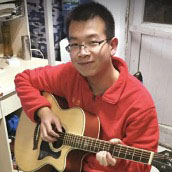
\includegraphics[width=3cm]{Images/自我介绍1.jpg}
        \end{figure}

        \begin{block}{\tiny{研究方向}}
            \small{生物信息学 | 基因编辑}
        \end{block}
        \bigskip
        \bigskip
        \bigskip
        \bigskip
        \bigskip
        \bigskip
        \bigskip
        \bigskip
        \bigskip
        \bigskip
        \bigskip
        \bigskip
        % col 2
        \column{0.7\textwidth}

        \begin{block}{\tiny{学习经历}}
            \begin{itemize}
                % \tiny
                \item {2014 $ \sim $ 2019 \quad 西北农林科技大学(学士)}
                \item {2016 $ \sim $ 2018 \quad 中国农业大学 (交换生)}
                \item {2019 $ \sim $ 至今 \quad 清华大学 博士研究生(PTN项目)}
                \item {2020 $ \sim $ 至今 \quad 北京大学 (联合培养)}
            \end{itemize}
        \end{block}
        \begin{columns}
            \column{0.4\textwidth}
            \begin{figure}
                \centering
                
\includegraphics[width=3cm]{Images/自我介绍2.png}
            \end{figure}
            \column{0.4\textwidth}
            \begin{figure}
                \centering
                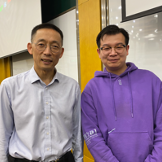
\includegraphics[width=3cm]{Images/自我介绍3.png}
            \end{figure}
        \end{columns}


        \bigskip
        \bigskip
        \bigskip
        \bigskip
        \bigskip
        \bigskip
        \bigskip
        \bigskip
        \bigskip
        \bigskip
    \end{columns}
\end{frame}
% 大家好!
% 今天是 2022-09-11 日
% 非常高兴能够作为主讲人给大家讲授这门
% 利用 Python 进行生信分析 的课程

% 在开始课程介绍之前,
% 首先请允许我做一个简短的自我介绍,也方便大家认识我
% 我叫赵华男
% 我在 2014 年参加高考,考入西北农林科技大学
% 在 2019 年,我从西北农林科技大学毕业,拿到了我的学士学位
% 期间我作为交换生在中国农业大学学习并顺利结业
% 在 2019 年,我通过北京大学,清华大学和北京生命科学研究所的联合招生项目
% 也就是 PTN 项目, 来到清华大学生命科学学院攻读博士学位
% 一年之后,也就是 2020, 我最终定导在北京大学我导师的实验室
% 我的研究方向呢,是生物信息学与基因编辑
% 好, 闲话少聊,我们开始这门课程的第一节,课程介绍
\subsection{课程介绍}
\begin{frame}[standout] 第一节 \quad 课程介绍 \end{frame}



\begin{frame}{这门课的开设目的}
    教大家使用 Python 写程序
    \begin{figure}
        \centering
        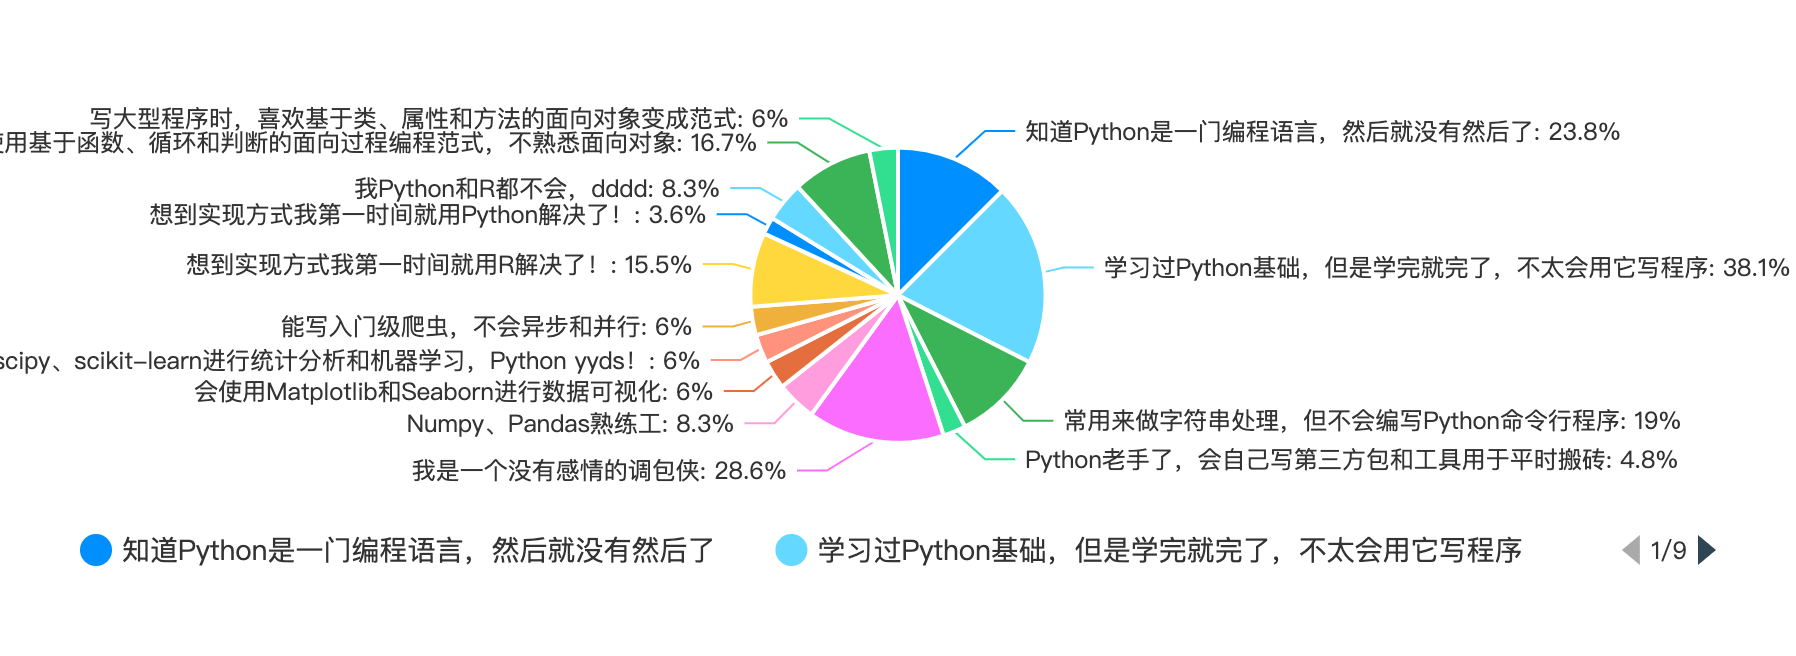
\includegraphics[width=15cm]{Images/level.png}
    \end{figure}
\end{frame}

% 正如课程介绍页面所述,这门课程的核心目的是教大家用 Python 写程序


\begin{frame}{这门课的开设目的}
    教大家使用 Python 写程序
    \begin{figure}
        \centering
        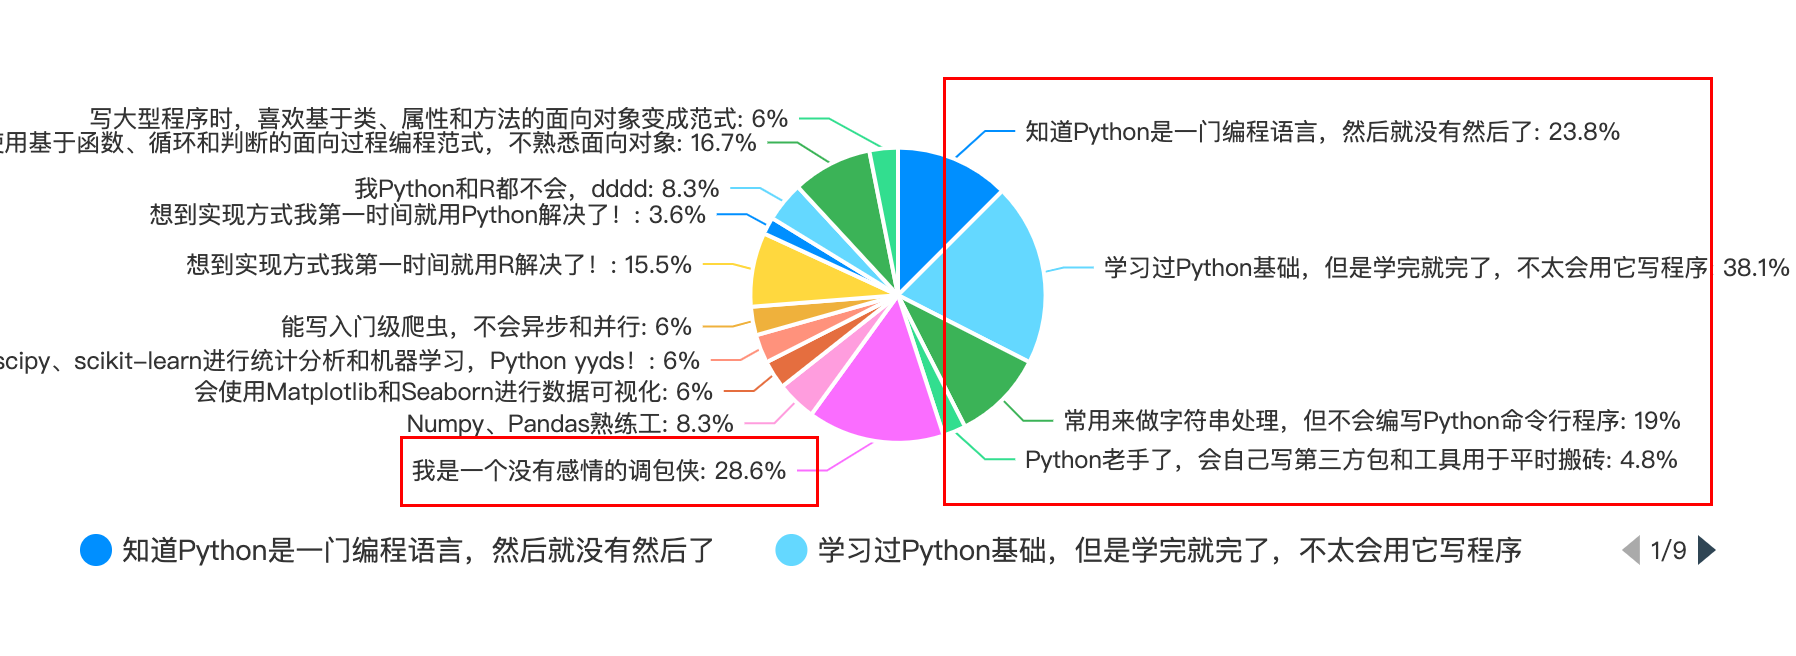
\includegraphics[width=15cm]{Images/level2.png}
    \end{figure}
\end{frame}
% 这张饼图是我做的一个问卷调查表,大家可以看到,
% 23.8%的同学没有学习过 Python
% 但是接近 40%的同学学习过 Python,但是并不会用它写程序
% 这门课程的目的,是为了解决大家关于 Python 学了不会用的痛点
% 或着是大家会用一些第三方包,但是 Python 使用和理解不够深入的问题


\begin{frame}{这门课的开设目的}
    教大家使用 Python 写程序 → 基础 + 有难度的几个实战项目
    \begin{figure}
        \centering
        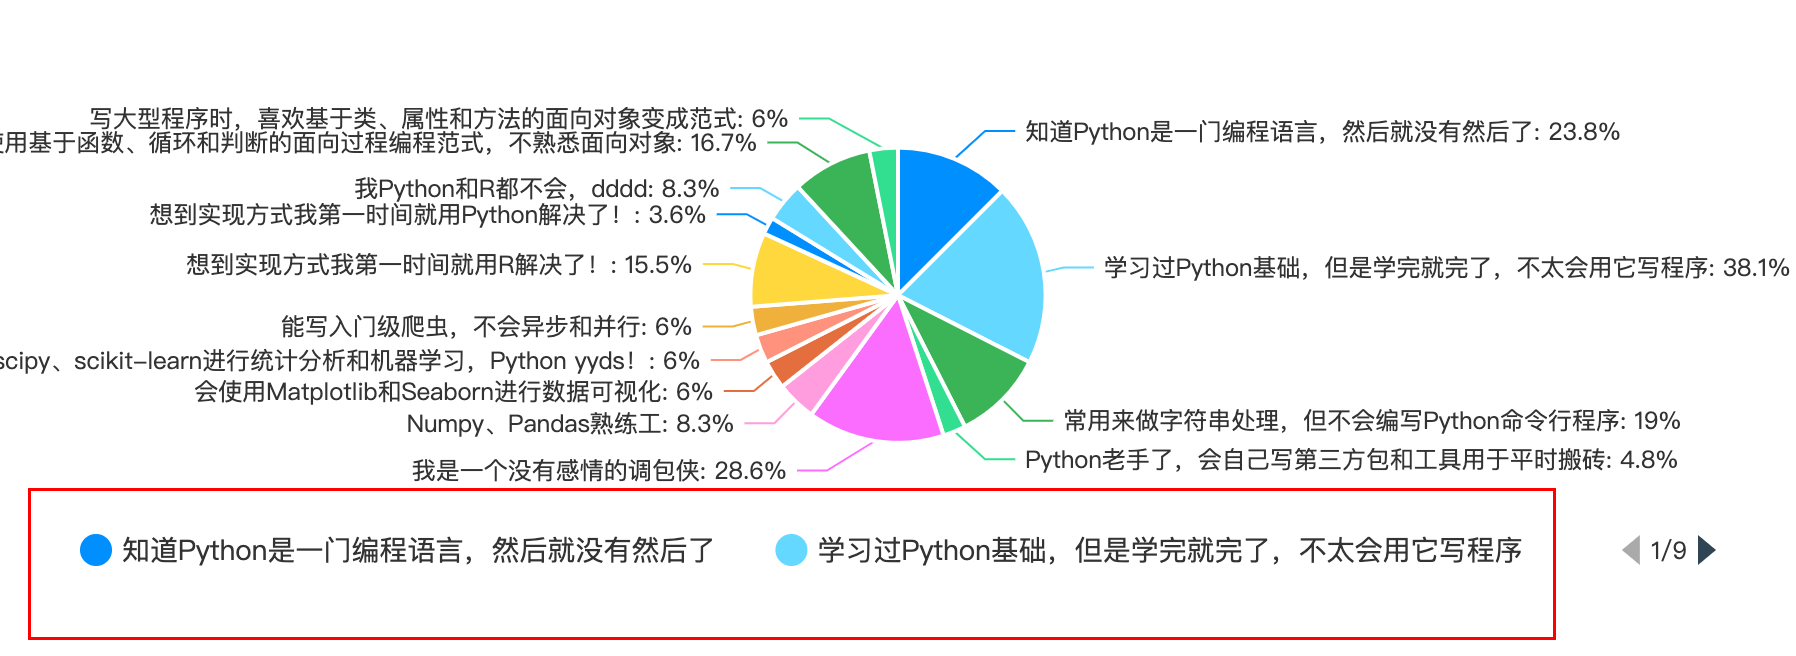
\includegraphics[width=15cm]{Images/level3.png}
    \end{figure}
\end{frame}

% 那这门课程, 我将会带着大家,用大量的时间,
% 使用 Python 完成几个比较有难度的生物信息学编程开发项目,
% 当然, 为了照顾一些零基础的同学,我们也将在课程一开始,
% 介绍操作系统的基本概念和 Python 的基础知识

% 我们先来看一下这门课程的设计思路

\begin{frame}{课程设计}
    \begin{itemize}
        \item 操作系统和编程语言 (Shell, PATH)
        \item Python 基础知识 + Python 进阶知识
        \item 编程实战(核心)
        \begin{itemize}
            \item 序列文件的处理(FASTA, FASTQ)
            \item BED 文件的操作与处理(BED)
            \item 基因注释文件处理(GFF, GTF)
            \item BAM 文件的解析与操作(SAM, BAM)
            \item 支持多核计算程序的编写
            \item 复杂命令行工具的编写与搭建
        \end{itemize}
    \end{itemize}
\end{frame}

% 首先,这是一门编程课,我们避免不了的要接触Linux 和命令行,
% 所以我们会简略地介绍一下操作系统和环境配置,和几个简单的 SHELL 命令,以及环境变量
% 接下来,我们将从 Python 的基础知识讲起, 过渡到Python进阶知识,也就是面向对象的一些概念
% 然后进入本课程的核心部分,编程实战,
% 在这个部分,我们针对生物信息学中常见的文件和分析需求,设计了六大实战模块
% 认真跟下来这几个项目,我相信大家
% 不但能获得项目开发能力的提高
% 还可以树立生物信息学分析的信心,针对常见分析需求,能够做到自信自己能搞定,成竹在胸

\begin{frame}[standout] Thank you! \end{frame}
% 好的,我们的第一节 课程介绍,就已经讲完了, 非常欢迎大家和我一起学习接下来的内容


 % 10 min

\section{第二节 \space 操作系统和编程语言} % 90 min
\subsection{Python语言简介}

\begin{frame}[standout] 第二节 \quad 操作系统和编程语言 \end{frame}

% 接下来,我们开始讲 第二节 操作系统和编程语言 的内容

\begin{frame}{Python语言的特点}
    \begin{figure}
        \centering
        
\includegraphics[width=8cm]{Images/Python.jpg}
    \end{figure}
    \small{
        \begin{itemize}
            \item Guido van Rossum在 1989 年创造了Python,在 1991 年将 Python 首次公开发行
            \item 跨平台、开源、解释型语言、高级语言
            \item 源代码可见
            \item 第三方包种类多, 可用底层语言(如C、Rust)重写关键代码
            \item 开发效率高,执行效率低
        \end{itemize}
    }
\end{frame}

% 在正式讲解操作系统之前, 我们先来简单了解一下 Python 的发展历史和特性
% 荷兰大叔 Guido van Rossum
% 在 1989 年创造了Python这门编程语言
% 并且在 1991 年将 Python 首次公开发行

% 经过了 30 年的发展,Python 已经成长为一个非常流行,跨平台,开源的编程语言
% Python 是一门解释型语言, 什么是解释型语言我们后面会讲
% 同时它是一门高级编程语言,拥有近似自然语言的表达能力

% Python 的源代码可见,不需要我们手动编译运行

% Python 也是一门胶水语言,能过融合其他高性能语言比如 C 的代码, 从而提高编写的程序性能,
% Python的开发效率很高, 由于表达能力强,内置工具包多等原因,
% 我们可以使用 Python快速搭建完成一个项目(大家注意看,他头发很多而且笑得很开心),

% 但是他的缺点也很明显,就是速度比较慢, 
% 而同样一个项目,使用如 C 语言去开发,可能开发时间就会很漫长,但是写出来的程序速度就会很快

\begin{frame}{Python语言的特点}
    \begin{itemize}
        \item Python 开发效率高,执行效率低 (科研,数据分析)
        \item C 开发效率低, 执行效率高 (高频量化交易)
        \begin{alertblock}{\small{执行效率对比}}
            \begin{itemize}
                \item  C \qquad \quad 10000行 \quad 0.01s
                \item  Java \quad \quad 1000行 \quad 0.05s
                \item  Python \quad 100行 \quad 0.1s
            \end{itemize}
        \end{alertblock}

    \end{itemize}
\end{frame}
% Python 的速度能有多慢呢, 我们列几个数字比较一下
% 当然不是严谨的,只是给大家一个概念
% C 或 Rust 等低级语言运行一万行代码,可能需要 0.01 秒
% -   提 JAVA 不提解释性语言
% 而 Java 运行 1000 行代码需要 0.05 秒 [注意,这里千万不要提 Java 的语言分类]
% 到了 Python 可能运行 100 行都需要 0.1 秒

% 但是不是说慢就一定不好啊,Python 100 行可以写出的程序,拿 C 来写可能就要写 1000 行
% 所以这是一个取舍,而对于生物信息学工作者来说,最重要的是能够快速实现想法,
% 等自己写的工具十分成熟和稳定了,才可能会考虑速度问题
\begin{frame}{Python擅长的领域}
    \begin{itemize}
        \item 爬虫
        \item Web后端开发
        \item 自动化运维、自动化测试
        \item 数据科学
        \item 机器学习
    \end{itemize}
\end{frame}

% 生物信息学是一个相对窄的领域, 那站在一个比较宏观的角度考虑, 
% Python 能做什么呢?
% 其实 Python 可以做的事情特别多
% 比如 Python 可以做爬虫, 网站后端开发,自动化运维和测试,数据科学和机器学习, 
% 那其实这里面的一些概念和方向大家可能不懂,或者不了解,
% 比如什么是爬虫什么是后端,什么是运维
% 其实, 在生物信息学上, Python 关于爬虫, 网页后端和其他方向都也有应用, 
% 我给大家举一些具体的例子感受一下

\begin{frame}{Python在生物信息学中的应用}
    \begin{columns}
        \column{0.4\textwidth}
        \begin{myoutline}[itemize]
            \1 数据获取(爬取UniProt)
                \2 \textcolor{lightgray}{爬虫}
            \1 \textcolor{lightgray}{Web前后端开发}
                \2 \textcolor{lightgray}{Django, Flask, 数据库\dots}
            \1 工作流程
                \2 Jupyterlab
                \2 \textcolor{lightgray}{Snakemake}
            \1 字符串处理
                \2 FASTA, FASTQ, BED-like, BAM/SAM
                \2 \underline{Biopython, Pysam}
            \1 数据分析机器学习
                \2 数据清洗, 数据分析, 可视化
                \2 \textcolor{lightgray}{特征工程, 机器学习}
        \end{myoutline}
        \column{0.6\textwidth}
        \begin{figure}
            \centering
            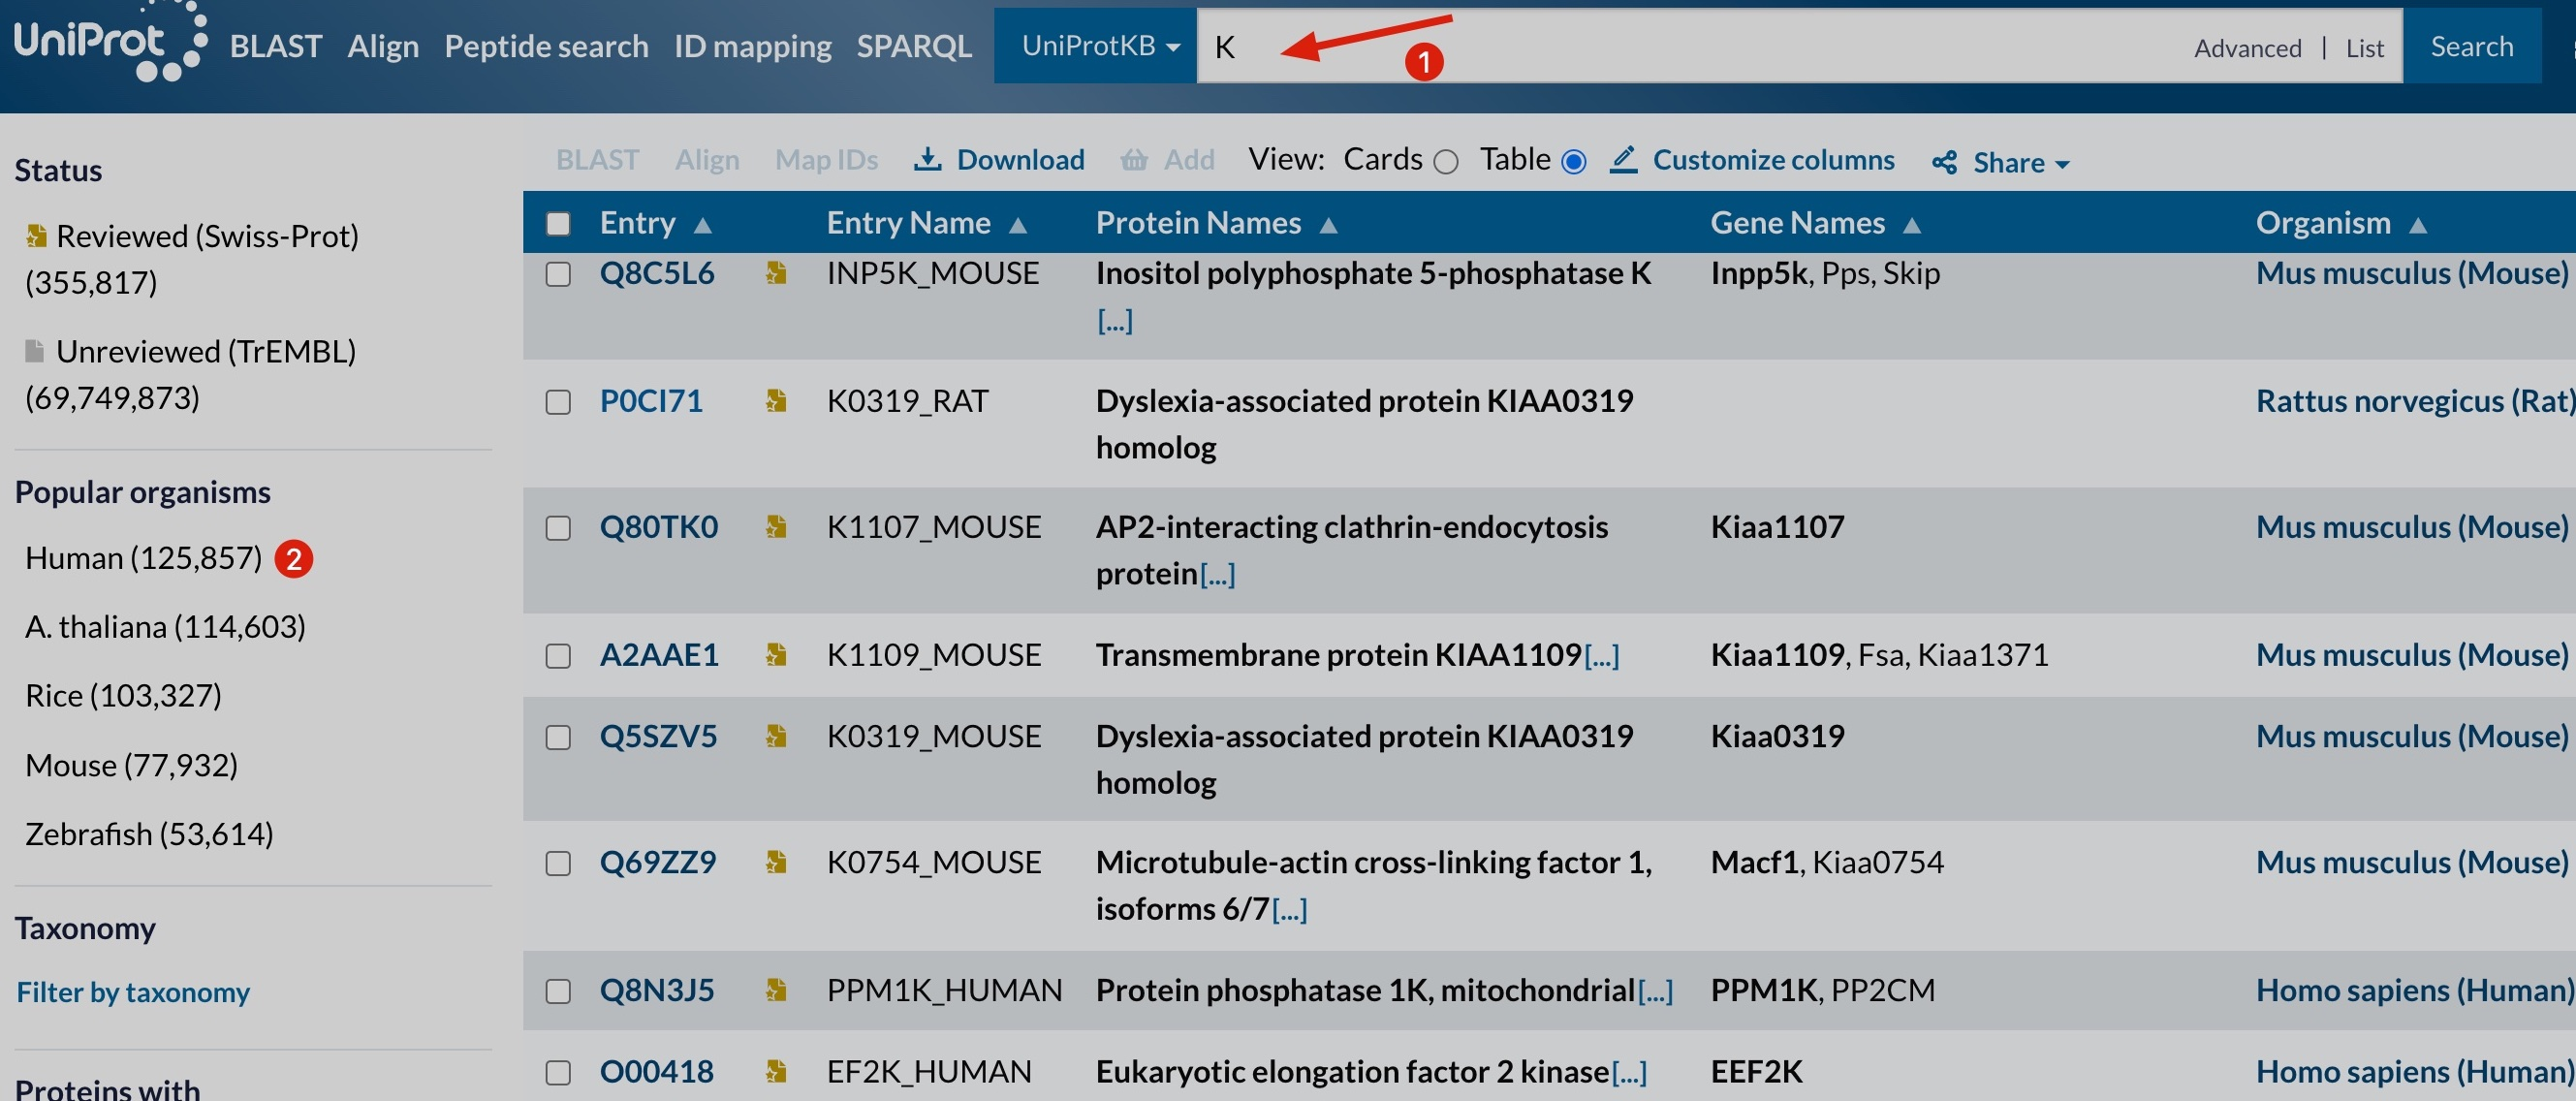
\includegraphics[width=8cm]{Images/uniprot.jpg}
            \caption{UniProt 蛋白数据库界面}
        \end{figure}
    \end{columns}

\end{frame}

% 比如,我们做数据分析,数据从哪里来,
% 假设要做一个蛋白结构预测的机器学习模型,那么我们需要大量的蛋白结构数据
% 一般我们获取一个蛋白结构可以去 UniProt 这个网页数据库中去检索然后使用鼠标操作下载
% 而如果我们需要几十万个蛋白,总不能一遍一遍点击,这样点到明年也下载不完
% 而爬虫就可以自动的帮我们打开浏览器操作网页,在很短的时间内访问并下载完这几十万个蛋白晶体结构
% 可以使用 Python开发爬虫来从公共网络中自动获取数据

\begin{frame}{Python在生物信息学中的应用}
    \begin{columns}
        \column{0.4\textwidth}
        \begin{myoutline}[itemize]
            \1 数据获取
                \2 \textcolor{lightgray}{爬虫}
            \1 \textcolor{lightgray}{Web前后端开发}
                \2 \textcolor{lightgray}{Django, Flask, 数据库\dots}
            \1 工作流程
                \2 Jupyterlab
                \2 \textcolor{lightgray}{Snakemake}
            \1 字符串处理
                \2 FASTA, FASTQ, BED-like, BAM/SAM
                \2 \underline{Biopython, Pysam}
            \1 数据分析机器学习 \\ (AlphaFold2$_{TensorFlow}$)
                \2 数据清洗, 数据分析, 可视化
                \2 \textcolor{lightgray}{特征工程, 机器学习}
        \end{myoutline}
        \column{0.6\textwidth}
        \begin{figure}
            \centering
            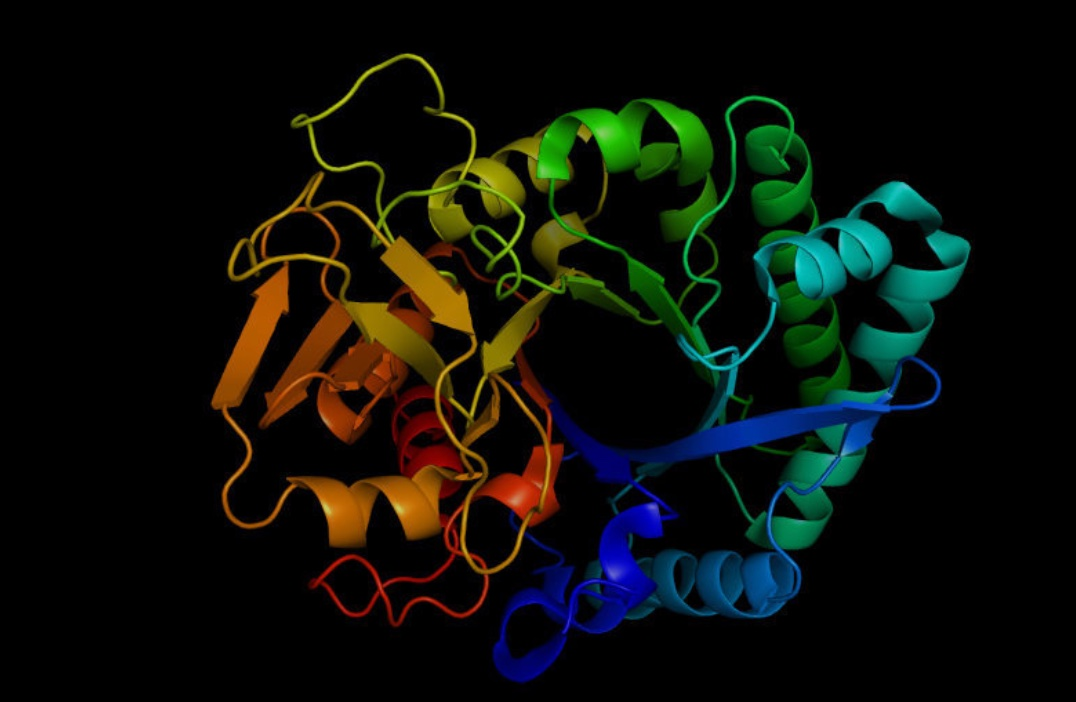
\includegraphics[width=8cm]{Images/alphafold.jpg}
            \caption{AlphaFold2 蛋白结构预测}
        \end{figure}
    \end{columns}
\end{frame}

% 那使用爬虫获取完这么多数据,就可以去使用机器学习模型进行结构预测,
% 现在大火的 AlphaFold2 就是一个预测蛋白结构的工具,
% 你可以把一个氨基酸序列输入给 AlphaFold2,经过计算它会告诉你这个氨基酸序列能折叠成什么样的三维结构,
% AlphaFold2 就是使用了大量晶体结构数据,
% 利用 Python 中很流行的一个机器学习框架,
% 叫 TensorFlow 的框架,经过大量数据的训练最终完成的机器学习模型

\begin{frame}{Python在生物信息学中的应用}
    \begin{columns}
        \column{0.4\textwidth}
        \begin{myoutline}[itemize]
            \1 数据获取
                \2 \textcolor{lightgray}{爬虫}
            \1 \textcolor{lightgray}{Web前后端开发} \\(AnnoLnc2)
                \2 \textcolor{lightgray}{Django, Flask, 数据库\dots}
            \1 工作流程
                \2 Jupyterlab
                \2 \textcolor{lightgray}{Snakemake}
            \1 字符串处理
                \2 FASTA, FASTQ, BED-like, BAM/SAM
                \2 \underline{Biopython, Pysam}
            \1 数据分析机器学习
                \2 数据清洗, 数据分析, 可视化
                \2 \textcolor{lightgray}{特征工程, 机器学习}
        \end{myoutline}
        \column{0.6\textwidth}
        \begin{figure}
            \centering
            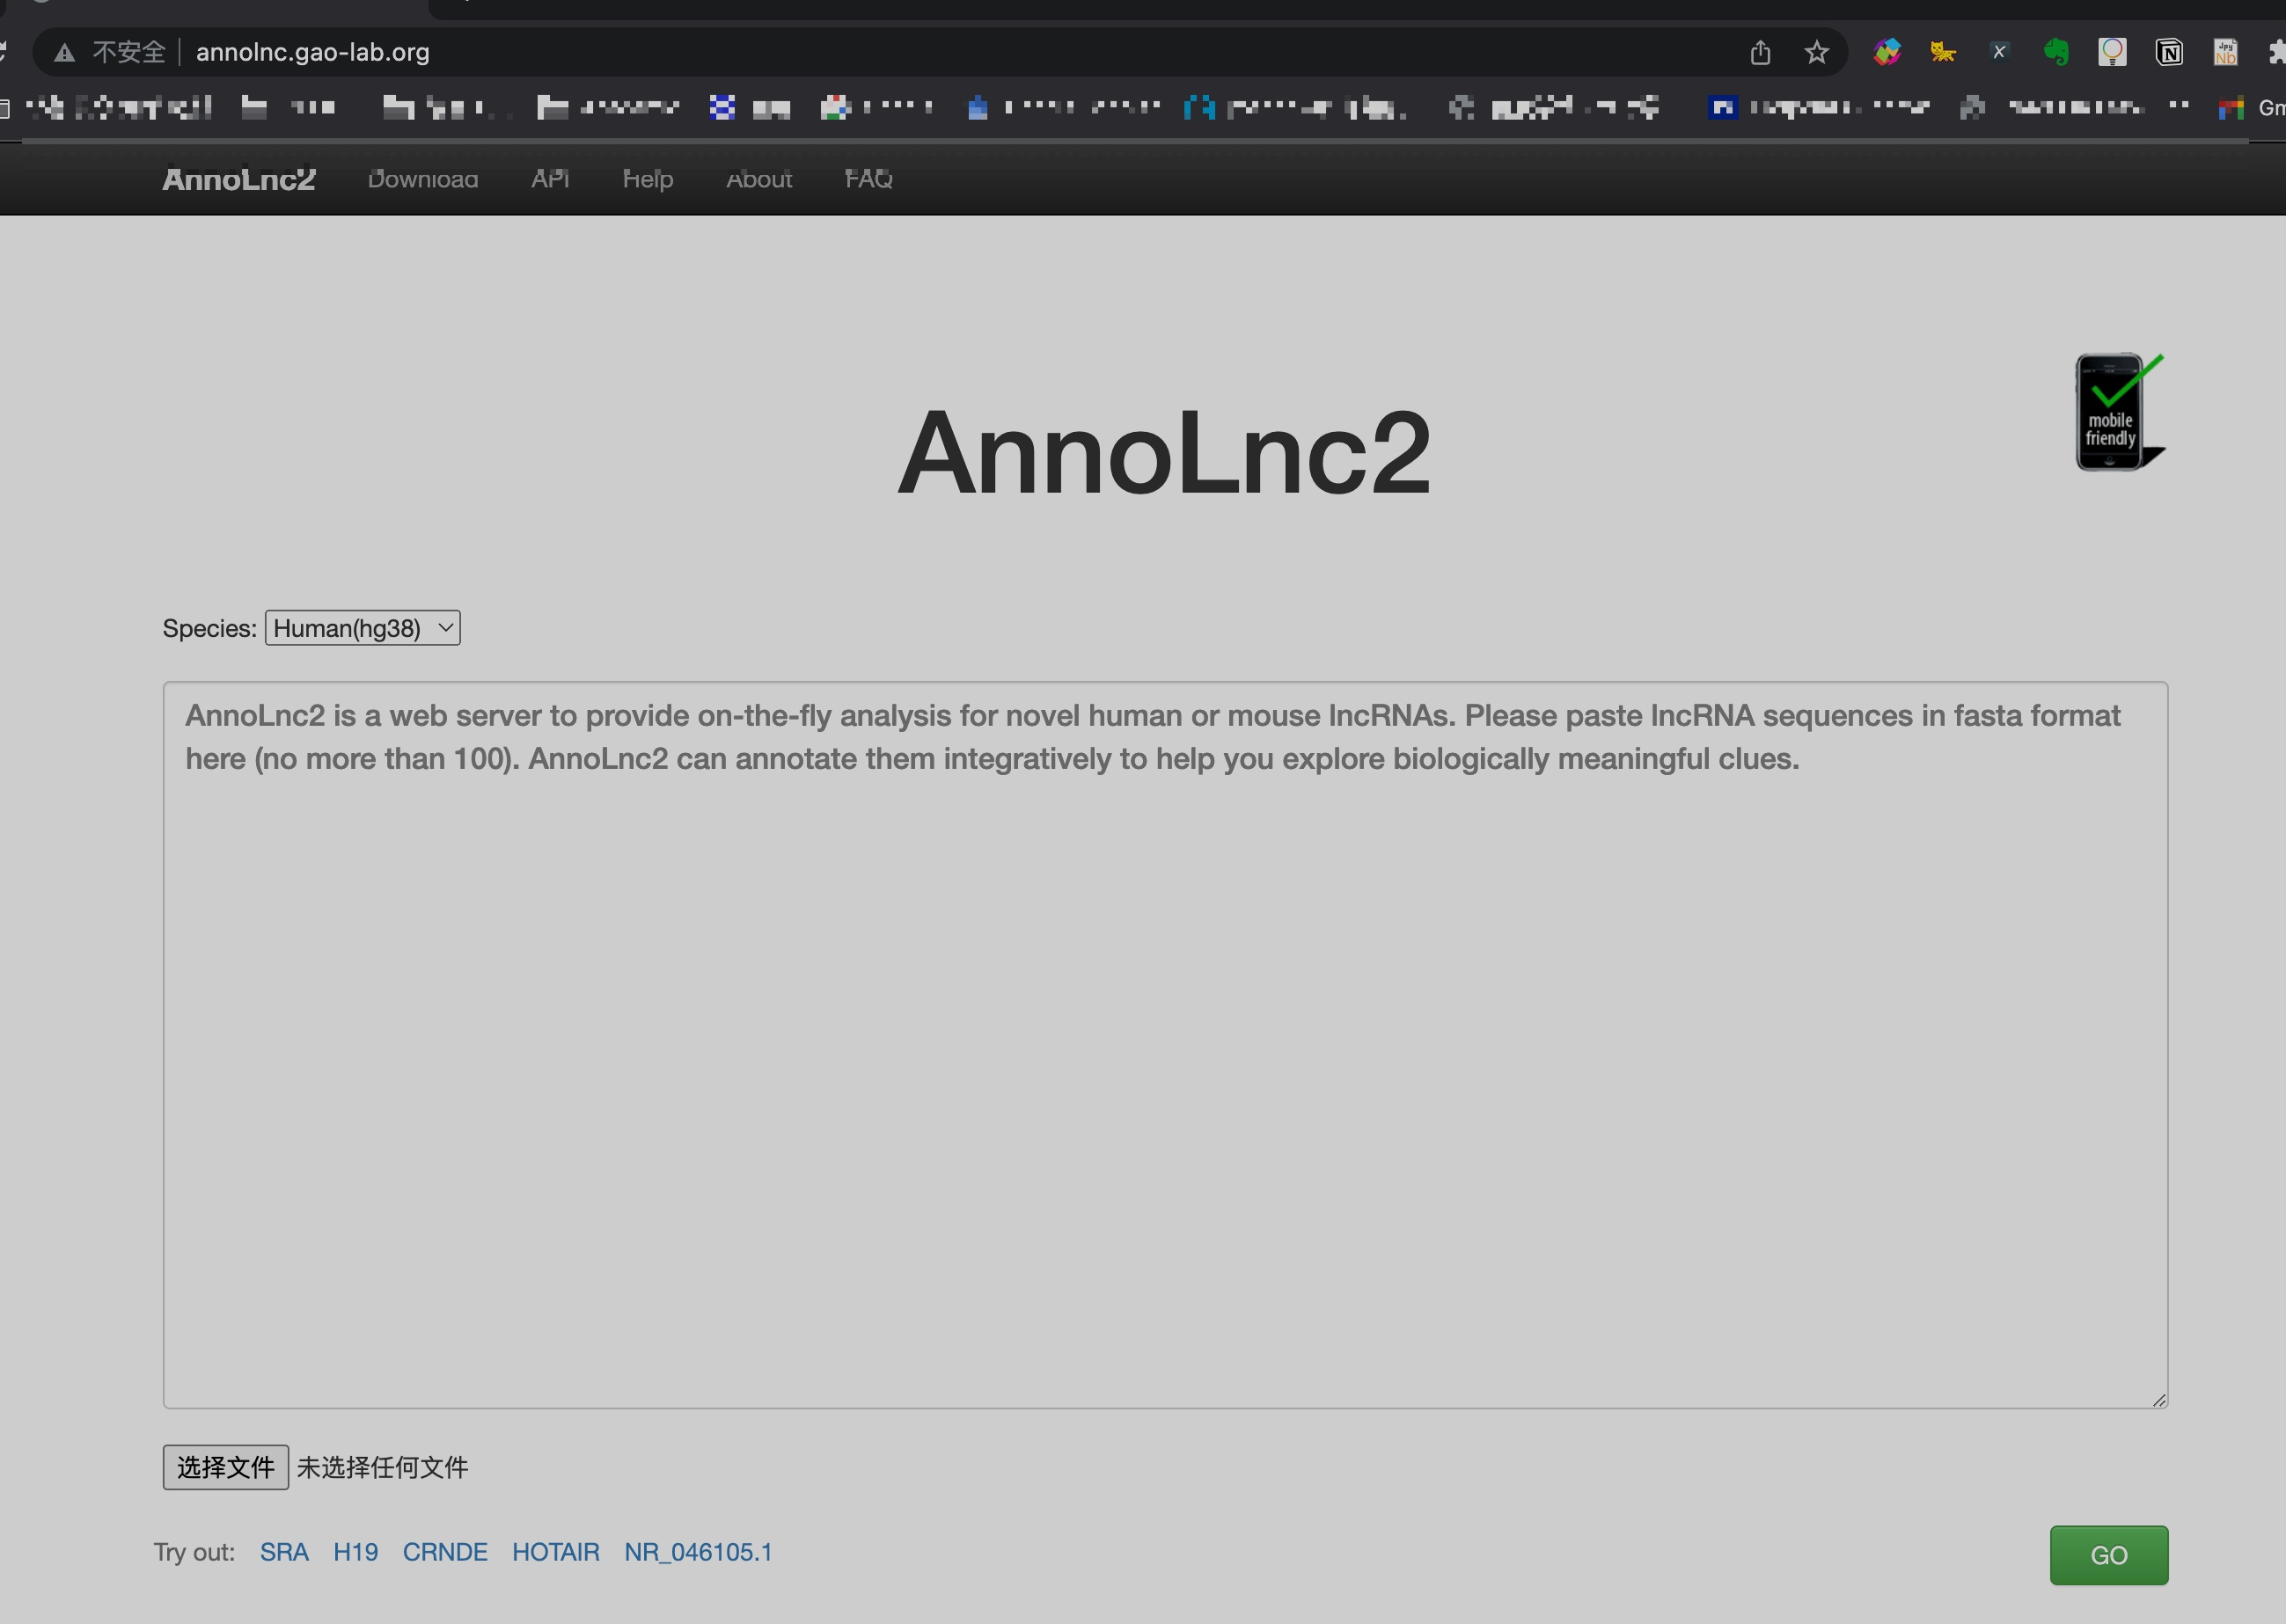
\includegraphics[width=8cm]{Images/annolnc2.jpg}
            \caption{AnnoLnc2 lncRNA 网页端分析工具}
        \end{figure}
    \end{columns}

\end{frame}

% 再比如, 北京大学的高歌老师课题组使用 Python 开发了一个网页端的生物信息学分析工具
% 叫做 AnnoLnc2, 你看名字就知道这个工具可以用来进行 LncRNA 相关的分析

\begin{frame}{Python在生物信息学中的应用}
    \begin{myoutline}[itemize]
        \1 数据获取
            \2 \textcolor{lightgray}{爬虫}
        \1 \textcolor{lightgray}{Web前后端开发}
            \2 \textcolor{lightgray}{Django, Flask, 数据库\dots}
        \1 工作流程
            \2 Jupyterlab
            \2 \textcolor{lightgray}{Snakemake}
        \1 字符串处理 \textcolor{red}{(强项)}
            \2 FASTA, FASTQ, BED-like, BAM/SAM
            \2 \underline{Biopython, Pysam}
        \1 数据分析机器学习
            \2 数据清洗, 数据分析, 可视化
            \2 \textcolor{lightgray}{特征工程, 机器学习}
    \end{myoutline}
\end{frame}

% 其实 Python 一个特性就是它是对字符串进行处理的能力非常强大
% 而很多生物信息学文件格式都是以文本为基础的格式
% 而使用 Python,就能比较容易的对这些文本文件进行处理
% 字符串处理也是我们这门课程的核心内容
% 而同时 Python 中也有比如 Biopython 和 Pysam 的第三方包
% 也可以使用这些包来对序列文件和 BAM 文件进行比较好的处理
% 最后就是, Python 中的 Jupyterlab 这个 IDE 工具,以后我会详细讲, 
% 它可以帮助我们进行数据分析和项目管理
% 而 Snakemake 就是基于 Python 编写的一个命令行的流程控制工具,
% 在生物信息学分析流程的标准化中有非常广泛的应用

% 这里标灰色的部分我们这门课暂时不涉及,而黑色字体所述的内容,在后面的课程内容中都会涉及

% 好,我们简单介绍完了 Python 的发展历程和Python 能够做的事情
 % 10min
\subsection{三大系统}

\begin{frame}{从 Windows 1.0 到 Windows 11}
    \begin{columns}
        % col 1
        \column{0.3\textwidth}
        \begin{figure}
            \centering
            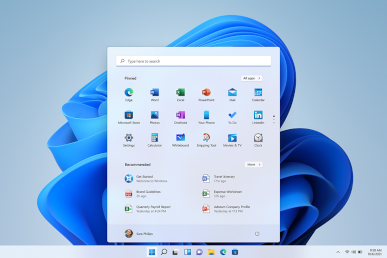
\includegraphics[width=5cm]{Images/windows5.png}
            \caption{Windows 11}
        \end{figure}

        % col 2
        \column{0.6\textwidth}
        \begin{figure}
            \centering
            
\includegraphics[width=0.1\linewidth]{Images/windows3.jpg}
            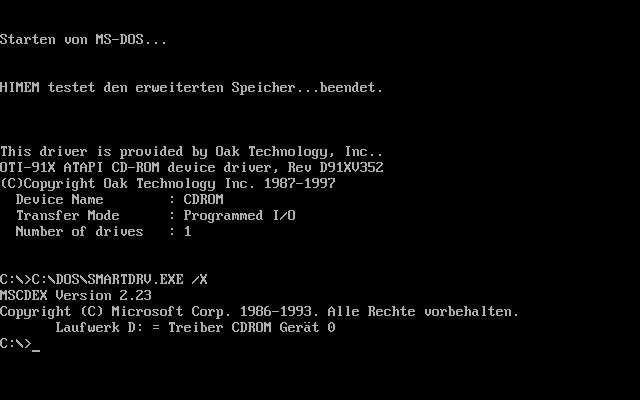
\includegraphics[width=5.2cm]{Images/windows4.png}
            \caption{MS-DOS 命令行界面}
        \end{figure}
        \tiny{现在在 Windows 系统中的 \textcolor{red}{PowerShell} 已经取代了 CMD成为新一代壳程序(Shell), 但是 CMD 仍然集成在操作系统中}
    \end{columns}
    \footnotenoindex{https://zh.wikipedia.org/wiki/Microsoft\_Windows}
    \footnotenoindex{https://zh.wikipedia.org/wiki/File:MS-DOS\_Deutsch.png}
    \footnotenoindex{https://zh.wikipedia.org/wiki/Windows\_11\#/media/File:Windows\_11\_Desktop.png}
\end{frame}

% 接下来, 我们来谈谈操作系统的概念和发展史
% 首先是我们最熟悉的 Windows 操作系统, 左边是现在最新的 Windows 11, 当然现在大部分人应该还在用 Windows 10
% 我们可以用鼠标单机和双击,完成对电脑绝大多数的操作

% Windows1.0 发布于 1985 年, 当年的 Windows 可不是能够用鼠标点点点的, 我们看右边
% 一开始 Windows 系统长这样, 就是一个干巴巴的 DOS 命令行
% 其实现在,这个命令行仍然存在, 也就是大家所知道的 CMD 命令行工具, 它被内置在现代 Windows 系统中
% 当年的电脑,一般人用不了,必须是受过专业训练的程序员才能通过键盘敲入命令的方式控制电脑

% 其实 CMD 它是一种壳程序,英文名叫 Shell 程序,什么是壳程序,或者说 Shell,我们后面会讲
% 那 Windows 发展至今, 其实 CMD 这个 Shell 已经逐渐被 PowerShell 这个功能更强大的 Shell 所取代了
% 不过 CMD 目前和 PowerShell 是在 Windows 中都存在的
% 请大家注意我提到的这个 Shell 概念,我们后面很多的课程都在 Shell 中完成

\begin{frame}{Windows, Linux, MacOS}
    \begin{columns}
        % col 1
        \column{0.5\textwidth}
        \begin{figure}
            \centering
            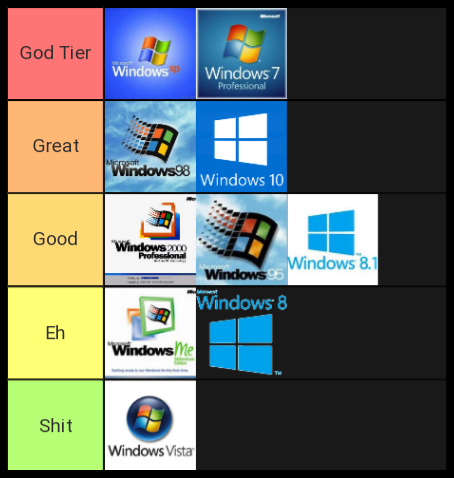
\includegraphics[width=3.5cm]{Images/windows.jpg}
            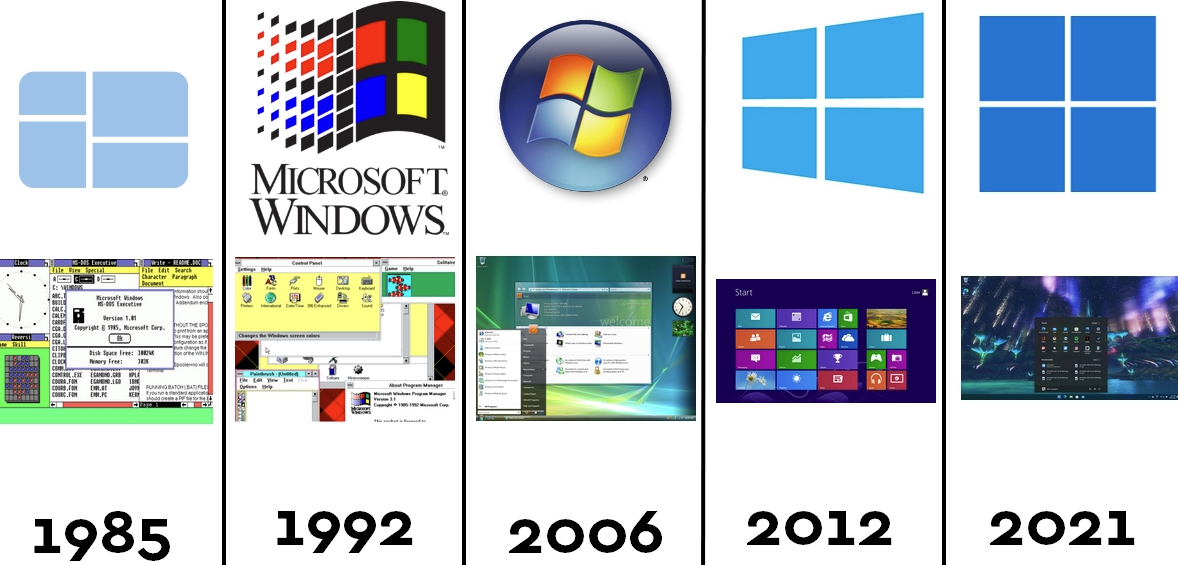
\includegraphics[width=3.5cm]{Images/windows2.jpg}
            \caption{Windows}
        \end{figure}

        % col 2
        \column{0.5\textwidth}
        \begin{figure}
            \centering
            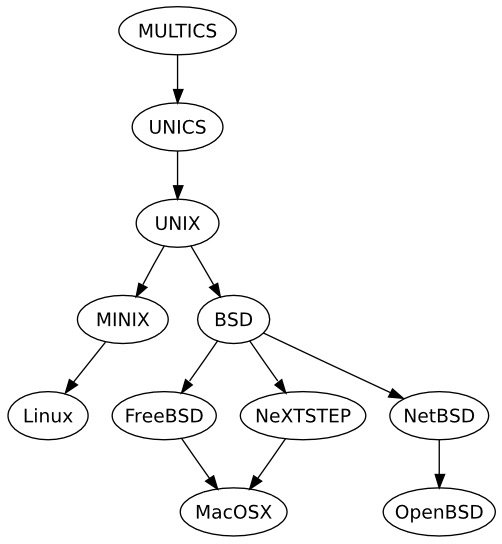
\includegraphics[width=5cm]{Images/unix.jpg}
            \caption{Linux, MacOS起源于UNIX}
        \end{figure}
    \end{columns}
\end{frame}
% 从 1985 年,Windows 系统诞生以后,Windows 就逐渐将系统做成了面向普通大众的,通过可视化的窗口点击来运行的系统,
% 并且每隔几年就推出新的版本,到了现在, Windows 系统已经占据了世界个人电脑操作系统的垄断地位

% 那除了 Windows, 剩下两个系统是什么?
% 在这门课里,三大系统指的分别是 Windows, Linux 和 MacOS

% 而 MacOS 和 Linux 就比较像了,他们都起源于一个叫做 Unix 的操作系统
% 我们刚刚讲到了 Windows 诞生于 1985 年, 而 Unix 系统的诞生时间比 Windows 还要早,
% Unix系统是在 70 年代初期, 在著名的美国贝尔实验室诞生的操作系统
% 贝尔实验室很有名, 它也是 C 语言的发明地,二极管的发明地, 这个实验室的很多研究造就了现在的计算机架构
% 我们说回 Unix
% 而经过几十年的发展, Unix 系统演化为了开源的 Linux 操作系统和专属于苹果公司闭源的 MacOS 操作系统.

\begin{frame}{Windows, Linux, MacOS}
    \begin{columns}
        \column{0.4\textwidth}
        Linux (Open source)

        \begin{itemize}
            \item 上百种不同的发行版\dots
            \item Ubuntu/Debian
            \item CentOS
            \item Android (Google Inc.)
            \item \underline{Shell: (sh, \textcolor{red}{bash}, zsh\dots)}
        \end{itemize}

        MacOS (Apple Inc.)
        \begin{itemize}
            \item Monterey
            \item \underline{Shell: (sh, bash, \textcolor{red}{zsh}\dots)}
        \end{itemize}
        \column{0.6\textwidth}
        \begin{figure}
            \centering
            
\includegraphics[width=6cm]{Images/distros_linux.jpeg}
            \caption{Linux发行版本}
        \end{figure}
    \end{columns}
\end{frame}

% Linux 由于是开源的,谁都能改来用,所以后面发展出了很多发行版本,
% 现在Linux 拥有上百种发行版本
% 比较有名气的比如罗列的 Ubuntu系统和 CentOS 系统
% 其实手机的 Android 操作系统也使用 Linux 的内核, 不过它由谷歌公司掌控, 是半开源状态

% 一般来说 Linux 的壳程序,也就是 Shell 默认是 bash,也可以设置为 sh,zsh 等其他 Shell程序

% MacOS 它是由苹果公司开发和掌控的, 是一个闭源的系统,
% 现在最新版本的系统是 monterey(蒙特雷)
% 而蒙特雷系统中默认的Shell程序 是 zsh,当然也可以设置为 sh 或者 bash

% 请注意我们反复提到了壳程序,或者说 Shell 程序这个概念
% 不断地让这个名字和大家见面,是因为 Shell 这个东西需要大家熟悉,我后面会细讲

% 毕竟 Linux 和 MacOS 是同源的, 可以使用相同的 Shell 程序是非常合理的
% 我们把 Linux比如 Ubuntu CentOS 和 苹果的 MacOS 这种
% 从 Unix 发展而来的操作系统统称为 类 Unix 操作系统

% 现在我们知道了 Windows, 类 Unix 包括 Linux 和 MacOS 
% 都是拥有 Shell 程序的,这是他们的相同点
% 那 Windows 和类 Unix 系统之间的区别是什么呢?

\begin{frame}{Windows与Unix-like系统之间的区别}
    \begin{columns}
        \column{0.5\textwidth}
        \small{
            \begin{table}[h]
                \begin{tabular}{|l|r|r|}
                \hline
                {\textbf{特点}} & {\textbf{Windows}} & {\textbf{Unix-like}} \\ \hline
                参考版本              & Windows10              & Ubuntu20.04              \\ \hline
                是否开源              & 否                      & 是                        \\ \hline
                路径表示              & 反斜杠                    & 斜杠                       \\ \hline
                文件结构              & 分区管理                    & 单一树状                       \\ \hline
                Shell 命令          & CMD 风格                 & Bash 风格                  \\ \hline
                \end{tabular}
        
                \textbf{\normalsize{Windows}}: 
                    \small{\underline{\textcolor{red}{C:}\textbackslash User\textbackslash zhaohuanan\textbackslash Document\textbackslash a.txt}}
                    
                    \small{\underline{\textcolor{red}{D:}\textbackslash somewhere\textbackslash Document\textbackslash b.txt}}

                \textbf{\normalsize{Ubuntu}}: 
                    \small{\underline{\textcolor{red}{/}home/zhaohuanan/Document/a.txt}}

                    \small{\underline{\textcolor{red}{/}home/someone/Document/b.txt}}
            \end{table}
        }
        \column{0.5\textwidth}

        \centering 
        Shell 命令举例

        \tiny{
            \begin{table}[]
                \begin{tabular}{|l|l|l|c|c|}
                \hline
                \textbf{操作}   & \textbf{\begin{tabular}[c]{@{}l@{}}Windows\\ CMD 命令\end{tabular}} & \textbf{\begin{tabular}[c]{@{}l@{}}Ubuntu\\ Bash命令\end{tabular}} & \textbf{相似} & \textbf{不同} \\ \hline
                切换目录          & cd                                                                & cd                                                               & √           &             \\ \hline
                打印当前目录        & cd                                                                & pwd                                                              &             & √           \\ \hline
                清除屏幕          & cls                                                               & clear                                                            &             & √           \\ \hline
                列出文件与子目录      & dir                                                               & \begin{tabular}[c]{@{}l@{}}ls \\ ls -l\end{tabular}              &             & √           \\ \hline
                列出所有文件与子目录    & dir /a                                                            & \begin{tabular}[c]{@{}l@{}}ls -a \\ ls -la\end{tabular}          &             & √           \\ \hline
                创建目录          & \begin{tabular}[c]{@{}l@{}}mkdir\\ md\end{tabular}                & \begin{tabular}[c]{@{}l@{}}mkdir\\ mkdir -p\end{tabular}         & √           &             \\ \hline
                删除目录          & \begin{tabular}[c]{@{}l@{}}rmdir\\ rd\end{tabular}                & \begin{tabular}[c]{@{}l@{}}rmdir\\ rm -rf\end{tabular}           & √           &             \\ \hline
                新建文件          & cd .> | notepad                                                           & touch                                                            &             & √           \\ \hline
                删除文件          & del                                                               & rm                                                               &             & √           \\ \hline
                拷贝文件          & copy                                                      & cp                                                               &             & √           \\ \hline
                在 Shell 中打印文件 & type                                                              & cat                                                              &             & √           \\ \hline
                移动文件          & move                                                              & mv                                                               &             & √           \\ \hline
                展示目录结构        & tree                                                              & tree                                                             & √           &             \\ \hline
                \end{tabular}
            \end{table}
        }
    \end{columns}
\end{frame}
% 首先,他们的区别是 Windows 是商业化的,闭源,微软公司以此盈利, Linux 是开源的,完全免费
% 第二个就是,类 Unix 操作系统和 Windows 的很经典的一个区别,就是文件的路径

% Windows 使用反斜杠来代表文件层级,如 C 盘的 User 目录下的 zhaohuanan 目录下的 Document 下的 a 这个文本文件
% 而windows 的文件系统是分区管理的,也就是说他的根目录出发点可以从 C 盘开始,一层一层往下找,找到 C 盘下的 User 下的 zhaohuanan 下的 Document 下的 a 这个文本文件
% 也可以从 D 盘出发,找打 somewhere 这个目录下的 Document 目录下的 b 这个文本文件
% Windows通过反斜杠来区分文件夹的层级, 而通过赋予这些磁盘 C 盘或者 D 盘或者 EFG 盘这种盘符,来进行分区管理

% 而类 Unix 系统则使用斜杠来代表文件层级, 且以斜杠开头, Unix 所有文件的地址都从这个斜杠开始,
% 而这个斜杠叫根目录
% 所以我们是从根目录出发,来到 home 这个文件夹中,找到 zhaohuanan 这个文件夹,再找到 Document这个文件夹,最终找到了 a 这个文本文件
% 而类 Unix 系统的特点就是你找什么文件和文件夹,都要从根目录出发,比如去找 b 这个文本文件夹,就还是从根目录出发,
% 从 home 到 someone 的 Document 文件夹下找到 b 这个 txt
% 类 Unix 系统是没有分区这个概念的,一切磁盘都从根目录开始寻址

\begin{frame}{文件系统结构}
    \begin{figure}
        \centering
        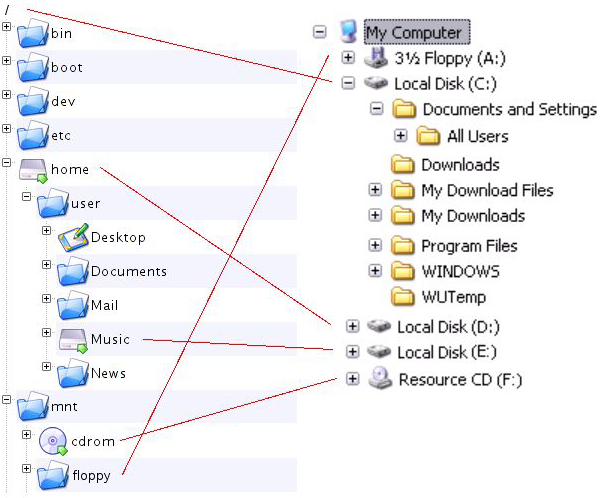
\includegraphics[width=0.55\linewidth]{Images/FileSystemWindowsVsLinux.png}
        % \tiny{\caption{左: 类 Unix 单一树状文件结构; 右: Windows 分区管理文件结构}}
    \end{figure}
    % \footnotenoindex{https://stevevincent.info/LUX205\_2017\_2.htm}
\end{frame}

% 我们用一张图,再来理解一下刚刚讲到的 Windows 和 Linux 文件系统的区别
% 左边是一个 ubuntu系统的文件路径
% 右边是一个windows 系统的文件路径
% 大家可以看到,在 Windows 这个系统中,一些文件路径是并列的,比如我们有一块硬盘分成了 C 盘和 D 盘,我们有另一块硬盘
% 分成一个 E 盘,我们还插入了一个 CD 光盘,系统给它分配了 F 盘, 还插入了一个软盘,给它分配了 A 这个盘符
% Windows 这里的这种文件地址都是以分配一个盘符为开始,然后向下寻址的,比如我要找 CD 光盘中的一个文件,那我要先跳转到 F 盘,再开始寻址

% 而 Linux 在这里就有理念上的不同了, 大家可以看到,我们同样挂载了一个 CD 光盘和一个软盘, 但是 Linux 系统会把他们放在 mnt 这个文件夹里面
% 而原本 Windows 一块硬盘分区为了 C盘 D 盘,在 Linux 就不去做拆分,而原本 Windows 中单独加的一块硬盘 E 盘,就可以
% 挂载到根目录下的 home 目录下的 user 下的 Music 这个路径

% 我们可以感受到 Linux 系统的设计理念,就是把一切都整合到一个树状分支路径中
% 而 windows 的理念就是,你每给我添加一个新的存储设备,我就给你分配一个根目录盘符和一个独立的树状分支

% 那讲到现在,相信大家对 Windows 和 Linux 的文件系统有一定的认识了
% 我们接下来对前面讲到的 Windows 和 Linux 的 Shell 命令以及路径进行一个简单的演示

\begin{frame}[standout]{路径演示}
    \begin{enumerate}
        \item 演示 Windows, MacOS, Linux(以Ubuntu为例)进入文件路径
        \item 打印当前目录, 切换目录
        \item 列出文件与子目录, 列出所有文件与子目录, 创建目录, 删除目录
        \item 新建文件, 拷贝文件, 移动文件, 删除文件
        \item 在 Shell 中打印文件, 清除屏幕
        \item 展示目录结构
    \end{enumerate}
\end{frame}

% -   怎么进入 Windows 的PowerShell
% -   怎么进入 Linux 和 MacOS 的 terminal
% 注意事项:
% 1. 字体调大
% 2. 事先准备好全屏的两个虚拟机可视化窗口
% 3. 争取所有操作全屏下进行

\begin{frame}{演示结论}
    \begin{myoutline}
        \1 类 Unix 系统和 Windows 系统在具体的特点上区别很大
            \2 路径分隔符不同
            \2 文件系统的结构不同
            \2 Shell 命令不同
        \1 但是这些操作系统的抽象层面上的逻辑都是类似的!
            \2 Shell 命令不同, 但具有相同或相似的功能, 如 type 和 cat
            \2 文件系统中的操作具有共性
                \3 文件/文件夹的创建/拷贝/移动/删除
                \3 目录切换
                \3 \dots
    \end{myoutline}
\end{frame}

% 虽然类 Unix 系统和 Windows 系统在具体的特点上区别很大,
% 比如路径分隔符一个用斜杠一个用反斜杠
% 文件系统的结构不同,一个用单一的树状结构,一个用分区结构
% Shell 命令也有很多都不一样

% 但是这些操作系统的抽象层面上的逻辑都是类似的
% 比如,虽然他们 Shell 命令不同, 但具有相同或相似的功能, 如 type 和 cat的功能都是打印文件内容到 Shell 程序中
% 再比如文件/文件夹的创建/拷贝/移动/删除,和目录切换

\begin{frame}{Unix系统层级}
    \begin{columns}
        \column{0.7\textwidth}
        \begin{figure}
            \centering
            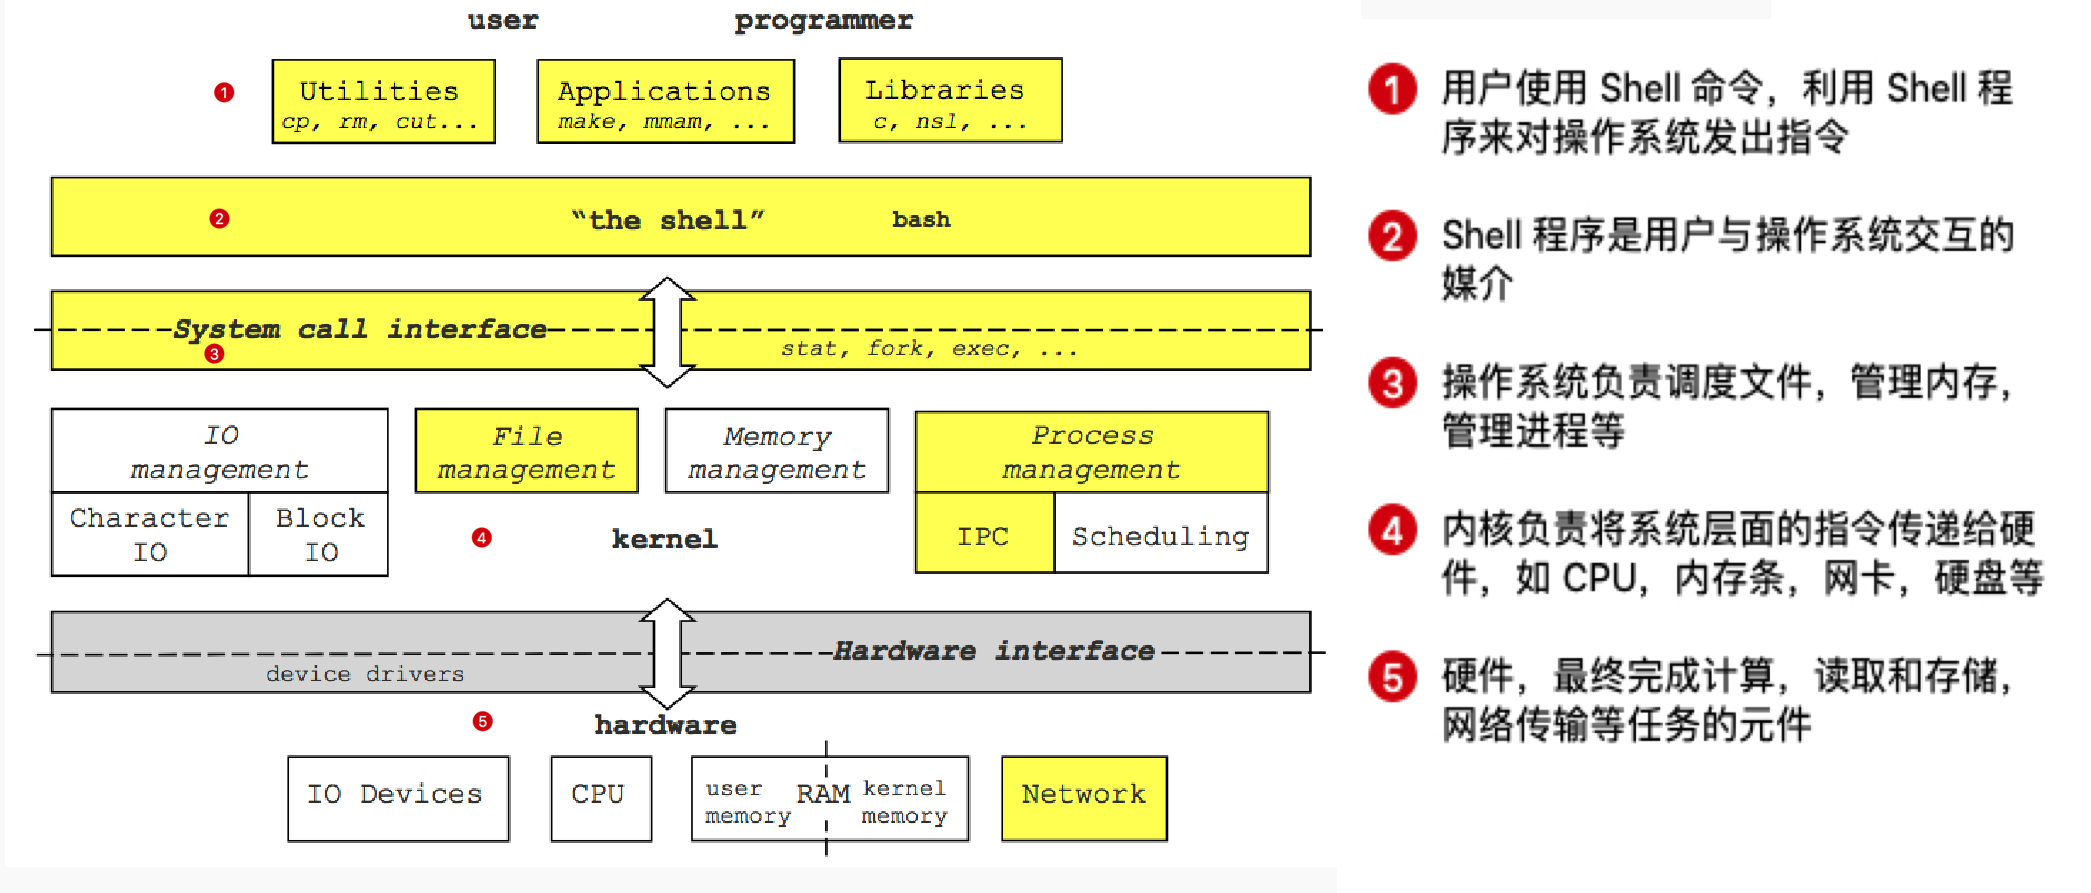
\includegraphics[width=1\textwidth]{Images/linux_work_order.png}
        \end{figure}
        \column{0.3\textwidth}
        \begin{myoutline}
            \1 用户空间
                \2 定义用户可访问的应用程序、库和标准实用程序
                \2 Shell也在``用户空间''中运行
            \1 内核空间
                \2 管理用户操作和硬件之间接口的操作系统的操作
                \2 操作系统的核心部分,其主要工作是将用户应用程序与底层硬件配对,并允许多个程序共享单个硬件组件
            \1 硬件
                \2 计算机的底层物理组件
                \2 输入/​​输出设备,如键盘和显示器、进行计算的 CPU、内存组件和网络接口
        \end{myoutline}
    \end{columns}

    \footnotenoindex{https://classes.adamaviv.com/ic221/s18/units/01/unit.html}
\end{frame}
% 其实 Windows 和 Unix 系统在宏观的逻辑上是非常相似的,
% 我们以 Unix 系统的层级为例来为大家介绍
% 我们使用 Shell 程序中的一个命令,比如说 cp 也就是拷贝文件这个命令,
% 第一步,这个命令会传递给 Shell 程序,
% 第二步,Shell 程序告诉操作系统, 要执行一个文件拷贝操作
% 第三部,这个操作会在操作系统层面发出指令给内核,
% 这个指令的内容包括了,调用一个 IO 指令,把原始文件读入内存, 然后再把内存中的信息写入硬盘
% 第四步,内核将这些指令真正转换为对硬件的一个个操作指令
% 第五步,硬件将这些指令进行执行

% 操作系统就像一个中间的传令兵一样,把我们想做的事情转换为对硬件的指令真正对硬件进行操作

% UNIX的系统层面上把上面这五步可以分为三个主要部分:

% 第一个部分是,用户空间:
% 用户空间定义用户可访问的应用程序、库和标准实用程序。
% Shell 壳程序就是一个用户空间的应用程序
% 我们写程序的时候,就是从用户空间开始操作的,
% 而不必不关心底层硬件之间的差异,那些由开发操作系统和驱动程序的人去关注。
% 那对我们来说, 执行 cp 命令在任何Unix 计算机上都一样,
% 但是由于每台计算机可能硬件不同, 系统底层给硬件的指令可能是不同的

% 第二个部分是内核空间:
% 这是指管理用户操作和硬件之间接口的操作系统的操作。
% 它是操作系统的核心部分,其主要工作是将用户应用程序与底层硬件配对,并允许多个程序共享单个硬件组件。

% 第三个部分是硬件:硬件是计算机的底层物理组件。
% 其中包括输入/​​输出设备,如键盘和显示器、进行计算的 CPU、内存组件和网络接口。

\begin{frame}{Linux的应用场景}
    \begin{myoutline}
        \1 桌面应用
            \2 Ubuntu
            \2 Archlinux
        \1 嵌入式应用
            \2 电梯、汽车、玩具、灯具、冰箱、空调、电饭煲等,都属于嵌入式概念的应用
        \1 服务器应用
            \2 开源, 免费, 无需考虑商业软件授权问题
            \2 高稳定性, 高可靠性
            \2 硬件要求低
    \end{myoutline}
\end{frame}
% 那我们讲了这么多类 Unix 系统的知识,
% 现在,我们来看一下其中的 Linux 系统到底被用来作什么
% 最容易理解的就是个人电脑,也就是桌面应用,这一点 Ubuntu 和 Archlinux等 Linux 系统发行版做得很好很漂亮
% 第二个应用就是嵌入式, 比如我们用的冰箱,洗衣机什么的,对话面板都是属于嵌入式开发,
% 最后,也是 Linux 最为核心的应用,就是用作服务器的系统,

% 讲到这里,我们基本上也进入了本课程的正题了,
% 大家都知道, 生物信息学相关的应用程序大都是基于 Linux 系统的,
% 手机上使用绝大多数需要服务器提供网络服务的 app, 比如 bilibil,知乎, 都是基于 Linux 系统的,
% Linux 系统能相比较于 Windows 和 MacOS,在服务器应用上占据绝大多数市场份额,
% 最大的原因有这三点,
% 首先,相对于 Windows 和 MacOS,Linux 是开源完全免费的
% 其次就是,Linux 系统非常稳定可靠,极少出现类似 Windows 打开一个大型论文文档, 编辑完还没保存就崩溃了这种问题
% 要知道,在大型的商业应用中,服务器如果宕机一个小时,可能对他们来说就会带来几百万的经济损失,
% 在稳定性上 Linux 相比 Windows 和 MacOS 都更值得信赖
% 最后一个点就是,跑起来一个Linux 系统,需要的硬件性能很低,可能一个 256M 的内存就可以跑得动 Linux,当然这是在不装 UI 界面的情况下,
% 而跑起来 Windows 系统起码也要 2G 的内存
% 综合下来, Linux 在服务器上的优势非常明显,所以现在也是占据了绝对主导的地位

% 好,我们花了较长时间来讲解三大系统这一个知识点,是希望大家在后面学习 Python 的过程中能
% 对整个计算机的组成有更深入的理解
% 对文件路径和文件结构有一定的认识
% 那,三大系统这个部分我们就讲完了 % 30 min
\subsection{Shell以及环境变量}
\begin{frame}{``the Shell''}
    概念: 在计算机科学中, Shell俗称壳(用来区别于核),是指``为使用者提供操作界面''的\textcolor{red}{软件}。
    \begin{columns}
        \column{0.5\textwidth}
        \begin{myoutline}
            \1 图形界面 Shell
                \2 Graphical User Interface Shell, GUI Shell
                \2 Windows
                    \3 Windows Explorer
                \2 Linux
                    \3 X-Window
                    \3 GENOME
                    \3 \dots
        \end{myoutline}
        \column{0.5\textwidth}
        \begin{myoutline}
            \1 命令行 Shell
                \2 Command Line Interface Shell, CLI Shell
                \2 Windows
                    \3 CMD
                    \3 PowerShell
                \2 Linux
                    \3 sh
                    \3 bash
                    \3 zsh
                    \3 \dots
        \end{myoutline}
    \end{columns}

    \tiny{传统意义上的 Shell 指的是命令行式的 Shell}

    \tiny{Shell 是一个操作界面, 里面的每一个命令是怎么来的?}
\end{frame}

% 接下来,我将为大家再正式地总结一下,我们多次提到的 Shell 概念,
% 其实前面的讲解中,我们一直没以一个概念的形式向大家展示 Shell 是什么,而是让大家去使用 Shell,去感受它是什么
% 那么其实大家应该已经有一个概念了,
% 也就是幻灯片所述的,在计算机科学中, Shell俗称壳(用来区别于核),
% 是指``为使用者提供操作界面''的软件
% 其实计算机系统发展到现在, Shell 被分为两大类
% 一个是图形界面的 Shell, 可以用鼠标点点点的,适合所有人使用, 比如 Windows 的文件浏览器,或者 Ubuntu 的 GENOME 图形界面
% 更传统上的是命令行界面的 Shell, 我们刚刚讲的,和练习的,都是命令行的 Shell
% 我们在 Windows 的 PowerShell, Ubuntu 的 bash, MacOS 的 zsh 中进行了练习

% 虽然广义上讲,为用户提供操作界面的软件就是 Shell, 
% 也就是说类似 Windows 的文件浏览器或者其他鼠标点点点就完成操作的这种界面也是 Shell,
% 但是, 大家基本上不这么说, 大家说的 Shell, 默认还是指的传统的命令行 Shell

% 那讲到这儿其实就引出了一个问题, 我们使用的 Shell, 它给我们提供了这么多命令和功能,
% 那这些命令是什么, 怎么来的呢?

\begin{frame}{命令与PATH}
    PATH是一个环境变量, PATH 中包含了\textcolor{red}{可执行文件} 的搜索路径

    \begin{columns}
        \column{0.5\textwidth}
            \tiny{
            当要求系统运行一个程序而没有告诉它程序所在的完整路径时,
            系统除了在当前目录下面寻找此程序外,还应到``PATH''中指定的路径去找。
            用户通过设置环境变量, 来更好的运行进程。
            }
        \column{0.5\textwidth}
        \begin{figure}
            \begin{flushright}
                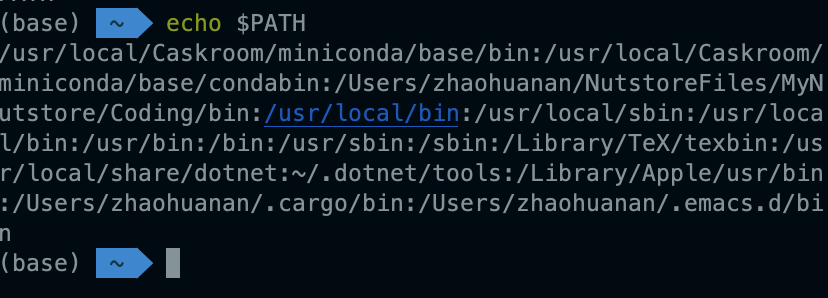
\includegraphics[width=1\linewidth]{Images/path.jpg}
            \end{flushright}
        \end{figure}
    \end{columns}
\end{frame}


\begin{frame}[standout]{PATH 的演示}
    \begin{myoutline}
        \1 MacOS/Linux
            \2 \$PATH
        \1 Windows
            \2 \%PATH\%
    \end{myoutline}
\end{frame}

% Windows 演示
% echo %PATH%
% C:\Windows\system32;C:\Windows;C:\Windows\System32\Wbem;C:\Windows\System32\W
% indowsPowerShell\v1.0\;C:\Windows\System32\OpenSSH\;C:\ProgramData\chocolatey
% \bin;C:\Program Files\OpenSSH-Win64;C:\opscode\chef\bin\;C:\Windows\system32\
% config\systemprofile\AppData\Local\Microsoft\WindowsApps;C:\Users\vagrant\sco
% op\shims_;C:\Users\vagrant\AppData\Local\Microsoft\WindowsApps;

% where python
% C:\Users\vagrant\AppData\Local\Microsoft\WindowsApps\python.exe

% 注释掉 Python 的 app path
% where python
% 找不着
% 再该回来
% where python
% 找到了

% MacOS 演示
% (base)  ~  PATH=/usr/local/Caskroom/miniconda/base/bin:/usr/local/Caskroom/miniconda/base/condabin:/Users/zhaohuanan/NutstoreFiles/MyNutstore/Coding/bin:/usr/local/bin:/usr/local/sbin:/usr/local/bin:/usr/bin:/bin:/usr/sbin:/sbin:/Library/TeX/texbin:/usr/local/share/dotnet:~/.dotnet/tools:/Library/Apple/usr/bin:/Users/zhaohuanan/.cargo/bin
% (base)  ~  which doom
% doom not found
% (base)  ✘  ~  PATH=/usr/local/Caskroom/miniconda/base/bin:/usr/local/Caskroom/miniconda/base/condabin:/Users/zhaohuanan/NutstoreFiles/MyNutstore/Coding/bin:/usr/local/bin:/usr/local/sbin:/usr/local/bin:/usr/bin:/bin:/usr/sbin:/sbin:/Library/TeX/texbin:/usr/local/share/dotnet:~/.dotnet/tools:/Library/Apple/usr/bin:/Users/zhaohuanan/.cargo/bin
% (base)  ✘  ~  PATH=/usr/local/Caskroom/miniconda/base/bin:/usr/local/Caskroom/miniconda/base/condabin:/Users/zhaohuanan/NutstoreFiles/MyNutstore/Coding/bin:/usr/local/bin:/usr/local/sbin:/usr/local/bin:/usr/bin:/bin:/usr/sbin:/sbin:/Library/TeX/texbin:/usr/local/share/dotnet:~/.dotnet/tools:/Library/Apple/usr/bin:/Users/zhaohuanan/.cargo/bin:/Users/zhaohuanan/.emacs.d/bin
% (base)  ~  which doom
% /Users/zhaohuanan/.emacs.d/bin/doom


\begin{frame}{演示结论}
    \begin{myoutline}
        \1 我们使用的命令,其本质是可执行文件
            \2 可执行文件具有完整的路径
            \2 可以直接使用命令的名称, 是因为其所在文件目录在 PATH 中
        \1 通过 PATH 中添加路径, 可以省略可执行文件的完整路径
            \2 当系统找不到用户输入的可执行文件时, 会在 PATH 中从前到后查找
            \2 当在PATH 中所有的路径下都找不到用户的可执行文件,会报错没有此可执行文件
        \1 安装程序时, 可以将可执行文件目录加入 PATH, 以方便使用此程序
    \end{myoutline}
\end{frame}


% 读 ppt 即可
% 那么到这里我们在操作系统和编程语言这一小节中, 关于 Shell 以及环境变量的知识就讲完了

 % 15min
\subsection{编译型语言与解释型语言}


\begin{frame}{编译型语言}

    编译型语言要求使用编译器一次性将所有源代码编译为一个可执行程序,一次编译可重复执行。

    \begin{myoutline}
        \1 编译型语言一般不能跨平台
            \2 编译出来的可执行程序不能跨平台:因为不同操作系统对可执行文件有着不同的要求,彼此之间不能兼容。
            \2 源代码不能跨平台: 不同操作系统下的函数、变量、api等可能会有不同。
        \1 代表语言:
            \2 C、C++
            \2 Golang
            \2 Rust
            \2 \textcolor{gray}{Java}?
    \end{myoutline}

\end{frame}
% Java即是编译型的,也是解释型语言
\begin{frame}{解释型语言}
    解释型语言是使用解释器一边执行一边转换,用到些源代码就转换哪些,不会生成可执行程序。
    \begin{myoutline}
        \1 解释型语言一般可以跨平台
            \2 跨平台是指源代码可以跨平台,解释器是不能跨平台的
            \2 源代码在不同操作系统中运行的结果相同
            \2 一个语言可以有不同的解释器用不同的语言实现这个解释器
        \1 代表语言:
            \2 C\#
            \2 JavaScript
            \2 PHP
            \2 Ruby
            \2 R
            \2 Python
    \end{myoutline}
\end{frame}
% 将高级语言的一条语句翻泽为机器语言,然后运行。且解释器发现错误, 程序会抛出异常或立即终止。

\begin{frame}{编译器与解释器}
    \begin{myoutline}
        \1 编译器 (编译型语言)
            \2 编译器在编译的过程中,读入源程序文件,输出一份等价的二进制可执行文件,就和笔译工作者一样,他们都会输出一份翻译后的文件。
        \1 解释器 (解释型语言)
            \2 解释器在解释的过程中,读入源程序文件,输出的是执行的结果,就和口译工作者一样,他们输出的是已经完成翻译的结果。
    \end{myoutline}
    \bigskip
    \bigskip
    \bigskip
    \centering

    \small{输出的不同是这两者最大的区别,一个会\textcolor{red}{输出用于执行的文件},另一个只会\textcolor{red}{输出运行的结果}。}
    \footnotenoindex{https://zhuanlan.zhihu.com/p/389371438}
\end{frame}


\begin{frame}{Python是一种解释型语言(了解)}
    \tiny{\textcolor{gray}{超纲内容, 入门同学可以先听不懂!}}
    \begin{myoutline}
        \1 导入大型包的时候第一次导入很慢, 以后会很快的原因?
        \1 Python并非完全是解释性语言, 它是\textcolor{red}{有编译}的:
            \2 Python在解释源程序时是分成两个步骤的:
                \3 首先处理py中的源代码, 编译生成一个二进制pyc\textcolor{red}{字节码文件} (main + module)
                \3 再对字节码进行处理, 才会生成CPU能够识别的机器码
                \3 有了module的字节码文件之后, 下一次运行程序时, 如果在上次保存字节码之后没有修改过源代码, Python 将会加载.pyc文件并\textcolor{red}{跳过编译module的字节码这个步骤}
                \3 当Python重编译时, 它会自动检查module源文件和字节码文件的时间戳
                \3 如果你又修改了module源代码,下次程序运行时,module的字节码pyc文件将自动重新创建
            \2 相对于py文件来说, 编译成pyc本质上和py没有太大区别, 只是对于\textcolor{red}{这个模块}的加载速度提高了;并没有提高代码的执行速度
            \2 通常情况下不用主动去编译pyc文件,除非需要隐藏源代码保持私密性
        \1 ``.pyc''文件可以对module导入进行加速, Python CLI 程序设计原则:
            \2 在 import 别的 py 文件(module, 模块)时,那个 py 文件会被存一份 pyc 加速下次装载
            \2 而主文件因为是直接执行而不是import导入所以不会保留pyc
            \2 这也是为什么写大程序原则是CLI入口代码尽量少的原因:
                \3 将主要代码都构建在模块中以加速程序启动
                \3 \textcolor{red}{因为CLI入口是当前运行的主程序, 并不会生成pyc!}
        \1 演示
    \end{myoutline}
\end{frame}

% (base)  Downloads  cat main.py
% from my_module import myprint

% myprint()
% (base)  Downloads  cat my_module.py
% def myprint():
%     print("a function in module!")

% 讲到这里,我们关于编译型语言和解释型语言的一些概念阐述就都说完了,
% 我们讲完系统,讲完编程语言的类别,那么下一步,我们要开始讲 Python 相关的内容了, 
% 其中会有很多实操课, 再进行下面的课程之前呢,希望能给大家提几个要求

% https://www.bilibili.com/video/BV1ex411x7Em?p=258&vd_source=e5c433ab0a245566be70de4210cd0727

\begin{frame}[standout]{接下来的要求}
    \begin{myoutline}
        \1 听课要求(零基础)
            \2 手机 No!
            \2 iPad No!
            \2 电脑 Yes!
        \1 养成记笔记的习惯
            \2 使用 Markdown 来记笔记
            \2 使用一个开箱即用的笔记工具
        \1 心态要求
            \2 看别人码代码是很枯燥的
            \2 动手自己跟着码代码, 获得成就感
            \2 程序员/生信工作者 90\%的时间是在解决问题的路上以及学习, 只有 10\%的时间在流畅地写代码, 要从Debug 的过程中得到进步和获得快乐!
        \1 不懂的概念和知识点
            \2 读报错信息, 动脑思考, 如果还不行↓
            \2 百度, 如果还不行↓
            \2 Google, 如果还不行↓
            \2 群里问, 请教师兄师姐
    \end{myoutline}
\end{frame}

% 希望大家, 尤其是零基础的同学, 看视频的时候能够边看边做, 手机和 iPad 学习编程都是非常低效的, 请拿起你的电脑
% 好记性不如烂笔头,多记心得体会和知识点, 至少以后有个印象回来翻翻, 记笔记的时候推荐使用支持 Markdown 的工具,比如某道云笔记,某象笔记,尽量开箱即用不花时间研究笔记工具
% 后面会有大量的代码课程, 其实看别人写代码是很容易走神儿的,所以希望你能自己动手敲一遍
% 最后一个点就是,遇到问题不要直接就问, 先思考,看报错信息,看不懂先把报错信息粘贴到百度或者谷歌上看看别人如何解决的
% 如果都没有解决你的问题, 来群里问

% 好的, 到这里我们就讲完了一些基本的要求





 %5min
\subsection{IDE介绍}
\begin{frame}{集成开发环境-IDE}
    集成开发环境(Integrated Development Environment, IDE): 

    \tiny{用于提供程序开发环境的应用程序,一般包括代码编辑器、编译器、调试器和图形用户界面等工具。
    集成了代码编写功能、分析功能、编译功能、调试功能等一体化的开发软件服务套件。
    所有具备这一特性的软件都可以叫集成开发环境。
    }

    \normalsize
    \begin{columns}
        \column{0.5\textwidth}

        流行的 Python IDE:

        \begin{myoutline}
            \1 \textcolor{blue}{PyCharm} (√)
            \1 \textcolor{blue}{VS Code}
            \1 \textcolor{pink}{Jupyter Lab} (√)
            \1 \textcolor{pink}{Spyder}

            \tiny{\1 IDLE, Sublime, Vim, Emacs\dots}
        \end{myoutline}

        \column{0.5\textwidth}
        
        \begin{figure}
            \centering
            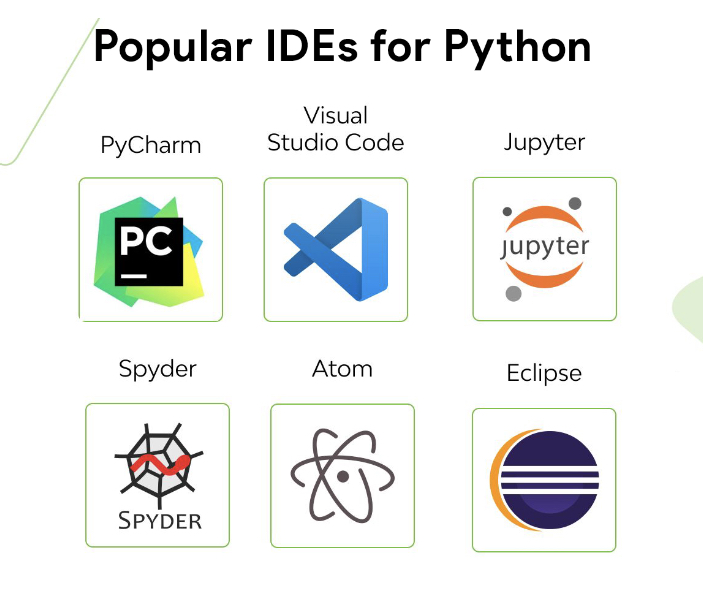
\includegraphics[width=0.7\linewidth]{Images/IDEs.jpg}
        \end{figure}
    \end{columns}

    \footnotenoindex{https://gknxt.com/python/whatisanide.php}
\end{frame}

% \1 PyCharm (工程, 业界)
% \1 VS Code (全能, 小巧)
% \1 Jupyter Lab (数据分析, 机器学习)
% \1 Spyder (数据分析, 机器学习)

% 接下来, 我们就从Python 的工作环境配置开始
% 首先, 我们先来学习一下什么是 IDE

% 以Pycharm,Jupyterlab,VScode
% IDLE, Sublime
% 区别在缩小,概念在弱化
% 会在以后的不同部分中融入进去 % 1min
\subsection{安装Python解释器}

\begin{frame}{Python的``解释器''}
    \begin{myoutline}
        \1 Python解释器(Interpreter)
            \2 解释执行Python源代码
            \2 官方版本的Python解释器是由 C 语言开发的(CPython)
            \2 其他版本的 Python 解释器:
                \3 IPython
                \3 PyPy
                \3 Jython 
                \3 IronPython 
        \1 当我们说, “安装Python”, 意思是安装Python的解释器
            \2 默认情况我们认为是安装官方版本的 CPython 解释器
            \2 默认我们使用的也是 CPython 
            \2 IPython 以及 Jupyter Notebook/Lab 是基于 IPython 的
        \1 IDE
            \2 PyCharm、VS Code、Spyder、Jupyter-lab
                \3 编写Python代码的工具
                \3 整合了Python解释器
                \3 代码提示功能
                \3 减轻工作量
    \end{myoutline}
\end{frame}
% CPython从名字就可以看出,CPython是由C语言开发的Python解释器,官方版本的Python解释器,也被称为标准的Python解释器,也是使用最为广泛的Python解释器。
% 当从Python官网下载并安装好Python之后,就直接获得了官方版本的Python解释器:CPython。
% 在cmd命令行下运行Python程序也是启动CPython解释器,而且CPython用>>>作为提示符。
% IPythonIPython是基于CPython的一个交互式的Python解释器。
% 简单理解,IPython和CPython在执行Python程序的功能上是一样的,但是IPython在交互方式上相比于CPython有增强。
% 而且IPython用In [序号]:作为提示符,这一点于CPython也有所不同。
% Anaconda中的Jupyter Notebook使用的就是IPython。
% PyPy是用Python实现的Python解释器,提供了JIT编译器和沙盒功能,能够对Python程序进行动态编译,
% 注意不是解释而是动态编译,在运行速度上比CPython快,显著提高了Python程序的执行速度。
% PyPy比CPython更加灵活,更易于使用和试验。
% 大部分Python程序都可以在PyPy上运行,但是由于PyPy和CPython的不同,可能会导致同一段Python程序在两种解释器下的运行结果会不同。
% 因此,如果想要在PyPy上运行Python程序,要先了解一下PyPy和CPython的不同。
% 而且PyPy对于Python第三方模块的支持还有不足。
% Jython,最初叫做JPython,由Java语言编写,是可以运行在Java平台上的Python解释器。
% Jython可以把Python程序编译成Java字节码来执行。
% JPython可以很好地与JVM集成,例如,使用JVM的垃圾回收和JIT,直接导入并调用JVM上其他语言编写的库和函数。
% IronPythonIronPython与Jython的作者都是 Jim Hugunin,与Jython类似,不同的是IronPython是运行在微软.Net平台上的Python解释,
% 可以把Python程序编译成.Net字节码来执行。
% 因此,IronPython能够很好地与.Net平台集成。

\begin{frame}[standout]{安装官方的Python解释器}
    \hyperlinkframeendprev{https://www.python.org/}
    \begin{myoutline}
        \1 Windows
        \1 MacOS
        \1 Linux
    \end{myoutline}
\end{frame}

\begin{frame}[standout]安装官方的Python解释器--Windows\end{frame}
\begin{frame}[standout]安装官方的Python解释器--Linux\end{frame}
\begin{frame}[standout]安装官方的Python解释器--MacOS\end{frame}


 % 10 min
\subsection{安装和配置conda环境}
\begin{frame}{Python的包管理工具}
    \begin{myoutline}
        \1 pip
            \2 查询包
            \2 安装包
            \2 卸载包
            \2 一定程度的自动配置环境依赖功能
        \1 venv
            \2 创建 Python 的虚拟环境
            \2 其余功能类似 pip
        \1 conda
            \2 查询、安装、卸载Python包
            \2 创建、切换、管理Python运行环境
            \2 命令行工具安装(生信、数据科学必会工具)
            \2 强大的自动配置环境依赖功能
    \end{myoutline}
\end{frame}

\begin{frame}{Conda简介}
    \begin{columns}
        \column{0.3\textwidth}
        \begin{myoutline}
            \1 Conda是一款环境管理工具
                \2 最流行的 Python 环境管理工具之一
                \2 开源的\textcolor{red}{软件包管理系统}和\textcolor{blue}{环境管理系统},
                    \3 用于安装多个版本的软件包及其依赖关系, 并在不同环境间切换
                    \3 Conda 是为 Python 程序创建的, 也可以打包和分发其他软件
                \2 Linux, MacOS 和Windows跨平台
            \1 Conda
                \2 Anaconda
                \2 Miniconda
        \end{myoutline}
        \column{0.7\textwidth}
        \begin{figure}
            \begin{flushright}
                
\includegraphics[width=0.5\linewidth]{Images/conda.jpg}

                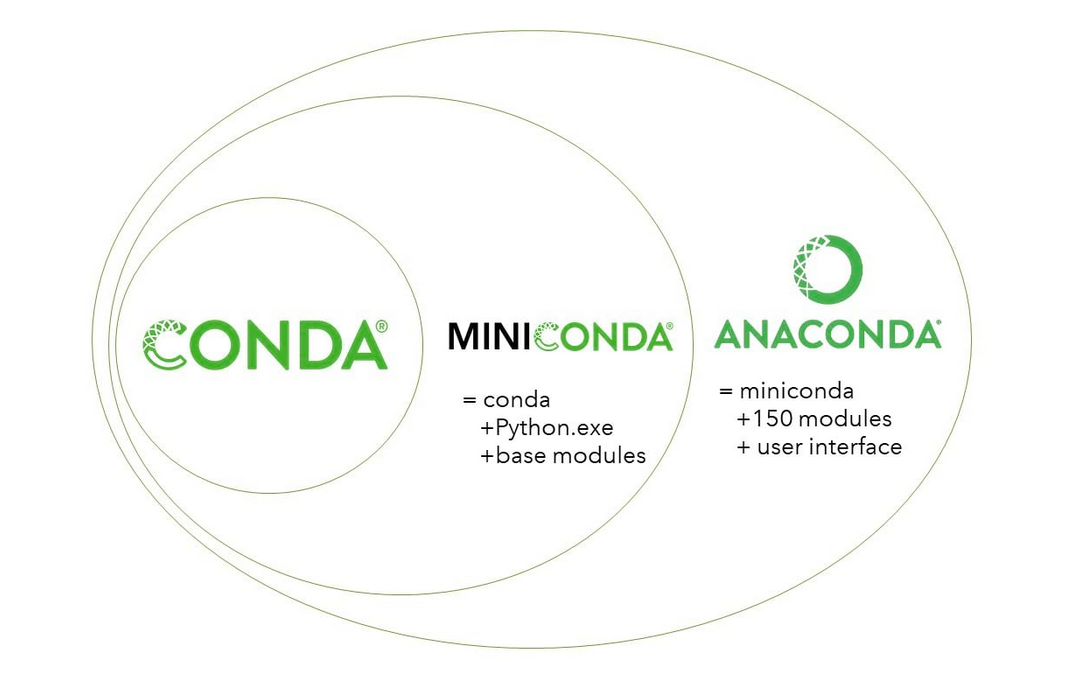
\includegraphics[width=0.9\linewidth]{Images/conda-vs-miniconda-vs-anaconda.png}
            \end{flushright}
        \end{figure}
    \end{columns}
    \footnotenoindex{https://www.zhihu.com/question/369468216/answer/997004544}
\end{frame}
% \2 miniconda windows 64位安装包大小约为55 Mb, 只包含了conda、python、和一些必备的软件工具
% \2 anaconda windows 64位安装包大小为470 Mb, 是miniconda的扩展, 包含了数据科学和机器学习要用到的很多软件


\begin{frame}[standout]{安装和配置conda环境}
    下载: tuna → conda → 清华大学 tuna 镜像站 → 搜索 conda → 选择 anaconda → 选择 miniconda → 选择``latest''版本!
    \begin{myoutline}
        \1 Windows
        \1 MacOS
        \1 Linux
        \1 用法
            \2 conda init 初始化 Shell 环境
            \2 创建一个指定 Python 版本的Conda环境
            \2 切换不同 Python 版本的Conda环境
            \2 对不同Conda环境安装不同版本的 Python 包
            \2 对一个Conda环境安装其他软件
    \end{myoutline}
    \footnotenoindex{https://conda.io/projects/conda/en/latest/user-guide/install/index.html}
    \footnotenoindex{https://mirrors.tuna.tsinghua.edu.cn/anaconda/archive/}
    \footnotenoindex{https://mirrors.tuna.tsinghua.edu.cn/anaconda/miniconda/}
\end{frame}

\begin{frame}[standout]安装和配置conda环境--Windows\end{frame}
\begin{frame}[standout]安装和配置conda环境--MacOS\end{frame}
\begin{frame}[standout]安装和配置conda环境--Linux\end{frame}

% Windows
% 选为所有人安装
% 加入环境变量!!!一定要选
% 注册 anaconda 为系统 Python!!
% install, next, finish
% myPC 属性 about 高级系统设置 环境变量



\begin{frame}[fragile]{Conda源--以MacOS 为例}
    \begin{columns}
        \column{0.82\textwidth}
        \begin{lstlisting}
# 清除之前残留的conda channels
rm -rf ~/.condarc
# 按顺序依次添加channel, 尽可能使用官方源
# 其他源常常在同步库的时候发生
# md5 值校验错误装不上包的问题!!!!
conda config --add channels defaults
conda config --add channels conda-forge
conda config --add channels bioconda
conda config --add channels r
# 备用, 清华源
# https://mirrors.tuna.tsinghua.edu.cn/anaconda/cloud/
# https://mirrors.tuna.tsinghua.edu.cn/anaconda/pkgs/
conda config --add channels https://mirrors.tuna.tsinghua.edu.cn/anaconda/cloud/msys2/
conda config --add channels https://mirrors.tuna.tsinghua.edu.cn/anaconda/cloud/conda-forge
conda config --add channels https://mirrors.tuna.tsinghua.edu.cn/anaconda/pkgs/free/
conda config --add channels https://mirrors.tuna.tsinghua.edu.cn/anaconda/pkgs/main/
#设置搜索是显示通道地址
conda config --set show_channel_urls yes
#查看当前conda配置
conda config --show channels
conda config --get channels
        \end{lstlisting}
        \column{0.12\textwidth}
        \begin{lstlisting}
cat ~/.condarc
# return
channels:
    - r
    - bioconda
    - conda-forge
    - microsoft
    - defaults
        \end{lstlisting}
    \end{columns}
\end{frame}


\begin{frame}[fragile]{pip源}
    \begin{lstlisting}
# PyPI 镜像在每次同步成功后间隔 5 分钟同步一次。
# 临时使用, 注意,simple 不能少, 是 https 而不是 http
pip install -i https://pypi.tuna.tsinghua.edu.cn/simple some-package

# 设为默认
# 升级 pip 到最新的版本 (>=10.0.0) 后进行配置:
python -m pip install --upgrade pip
pip config set global.index-url https://pypi.tuna.tsinghua.edu.cn/simple
# 如果您到 pip 默认源的网络连接较差,临时使用本镜像站来升级 pip:
python -m pip install -i https://pypi.tuna.tsinghua.edu.cn/simple --upgrade pip
    \end{lstlisting}
    \footnotenoindex{https://mirrors.tuna.tsinghua.edu.cn/anaconda/}
\end{frame}


\begin{frame}[fragile]{Conda, Pip的扩展用例}
    \begin{lstlisting}
# install mamba
conda install -c conda-forge mamba
mamba update -n base -c defaults conda
mamba install pandas
# conda 导出环境/导入环境
## 导出当前环境:
conda env export > requirements_conda.yml
## 导入环境:
conda env create -f requirements_conda.yml
## 备注:一些找不到的小组件直接删掉后再安装
# 滚回某个环境
conda list --revisions
conda install --revision=n
# 删除某环境
conda env remove -n learn

# pip 导出环境/导入环境
## 导出当前环境:
pip freeze > requirements.txt
## 导入环境:
pip install -r requirements.txt
    \end{lstlisting}
\end{frame} % 10 min
\subsection{安装和配置JupyterLab环境}

\begin{frame}[standout]{安装和配置JupyterLab环境}
    \begin{myoutline}
        \1 使用Conda 安装和配置JupyterLab
            \2 
        \1 JupyterLab 基本用法
            \2 ipynb
            \2 terminal
    \end{myoutline}
\end{frame}

\begin{frame}[standout]install JupyterLab--Windows\end{frame}

\begin{frame}[fragile]{install JupyterLab}
    \begin{columns}
        \column{0.45\textwidth}
        \begin{lstlisting}
conda install jupyterlab nodejs # nodejs > 12.14
pip install jupyterlab_theme_hale # theme
jupyter-lab --no-browser --port 8888 # run
# 启用extension manager

# func: Settings Editor Form UI
# setting:
{
    "settingEditorType": "json"
}
# func: File Browser
# setting: 
{
    "navigateToCurrentDirectory": true,
    "useFuzzyFilter": true,
    "showLastModifiedColumn": true,
    "showHiddenFiles": true,
}
        \end{lstlisting}
        \column{0.45\textwidth}
        \begin{lstlisting}
# func: Text Editor
# setting:
{
    "editorConfig": {
        "autoClosingBrackets": true, // 补全括号
        "codeFolding": true, // 代码折叠
        "cursorBlinkRate": 530,
        "fontFamily": null,
        "fontSize": null,
        "insertSpaces": true,
        "lineHeight": null,
        "lineNumbers": true,
        "lineWrap": "on",
        "matchBrackets": true,
        "readOnly": false,
        "tabSize": 4,
        "rulers": [],
        "showTrailingSpace": false,
        "wordWrapColumn": 80
    }
}
        \end{lstlisting}
    \end{columns}
\end{frame}

\begin{frame}[standout]install JupyterLab--MacOS\end{frame}

\begin{frame}{已经整合的优秀插件}
    \begin{figure}
        \centering
        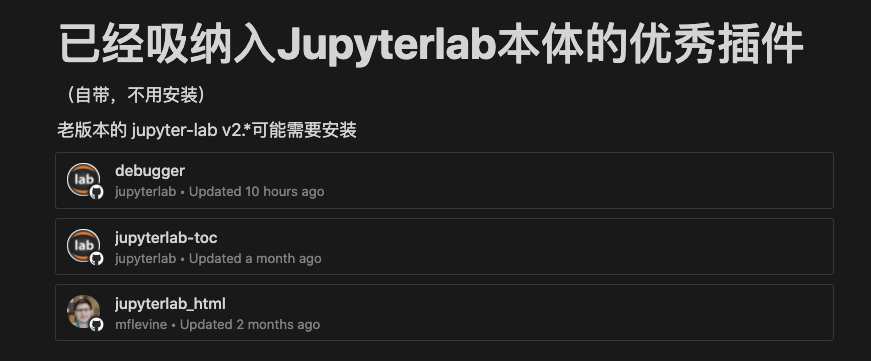
\includegraphics[width=0.99\linewidth]{Images/jupyterlabextension.jpg}
    \end{figure}
\end{frame}

\begin{frame}[fragile]{自动补全插件}
    \begin{columns}
        \column{0.45\textwidth}
        \begin{lstlisting}
pip install jupyterlab-lsp
pip install python-lsp-server pyright
conda install r-languageserver # 如果需要用 R


# func: Code Syntax 
# 启用或者关闭 lsp 自动补全
# true 为关闭,false 为开启
# setting:
{
    "disable": false,
}
        \end{lstlisting}
        \column{0.45\textwidth}
        \begin{lstlisting}
# func: Language Server
# setting:
{
    "language_servers": {
    "pyls": {
        "serverSettings": {
        "pyls.plugins.pydocstyle.enabled": true,
        "pyls.plugins.pyflakes.enabled": false,
        "pyls.plugins.flake8.enabled": true
        }
    },
    # 如果需要用 R
    "r-languageserver": {
        "serverSettings": {
        "r.lsp.debug": false,
        "r.lsp.diagnostics": false
        }
    }
    }
}
        \end{lstlisting}
    \end{columns}
\end{frame}
 % 10 min
\begin{frame}[standout] Q \& A! \end{frame}
\begin{frame}[standout] Thank you! \end{frame}

\section{第三节 \space Python基础知识} % 90 min
\subsection{Hello World!}

\begin{frame}[standout] 第三节 \quad Python 基础知识 \end{frame}

\begin{frame}{Hello World}
    \begin{myoutline}
        \1 提示: 输入法使用英文!
        \1 两种运行方式
            \2 python 的shell页面
                \3 ``交互式'', 输入一行, 按回车, 返回一次结果, exit()退出(演示)
                \3 应用" 在 python 中测试少量代码
            \2 python 源代码文件``.py''
                \3 编辑好每一行代码, 在命令行全部运行(演示)
                \3 本质: 使用安装在\textcolor{red}{指定路径下的} python \textcolor{red}{解释器} 运行指定目录下的``.py''源代码文件(文本文件)(演示)
            \2 源代码文件本质是``文本文件''(可以使用 cat 或者 type 命令打印到命令行)
        \1 知识点
            \2 ``123'' 字符串
            \2 123 整数
            \2 \# 注释
                \3 注释一行
                \3 行内注释
        \1 使用不同 IDE 进行演示并说明不同 IDE 运行逻辑
    \end{myoutline}
\end{frame}

% Windows
% (Python Shell)
% >>> print("Hello Python!")
% Hello Python!
% >>> print("Hello World!")
% Hello World!
% >>> print("Hello Windows!")
% Hello Windows!
% MacOS
% >>> print("Hello MacOS!")
% Hello MacOS!
% Linux
% >>> print("Hello Linux!")
% Hello Linux!

% Windows
% python 源代码文件``.py''
% cat .py
% print("Hello World!")
% print("Hello Python!")
% print(1 + 1)

% python test.py
% Hello World!
% Hello Python!
% 2
% MacOS

% PyCharm
% 新建项目, 选择解释器
% /usr/local/Caskroom/miniconda/base/bin/python /Users/zhaohuanan/Downloads/test_PyCharm/test.py 
% Hello PyCharm!

% Jupyter Lab 缩放 150%
% print("Hello Jupyter Lab!")
% 打印解释器位置

% Jupyterlab 笔记从这里开始!!!


% # Hello World

% ## 查看解释器位置
% 需要使用 sys 模块
% `sys.executable`是一个变量,记录了正在使用的 Python 解释器位置


% ```python
% import sys

% sys.executable
% ```

% ## Hello World in JupyterLab

% ## print
% - print是一个函数名
% - print()调用这个函数
% - print 函数的功能是将括号中的内容打印到命令行(Jupyterlab 中是打印到 Cell 下面)


% ```python
% print("Hello Jupyter Lab!")
% ```


% ```python
% print("123")
% print(123)
% # print(123)
% ```

% ## 注释
% - 在 Python 中,使用 `#` 进行注释


% ```python
% # 1
% ```


% ```python
% 1
% ```

% ## 字符串和数字
% - 使用`'', "", """"""`括起来的内容,为字符串
% - 像 `123` 这种的,就是整数, `123.45` 为浮点数, 它们都是数值型的变量

% ## 补充知识
% - 使用`""""""`三引号进行多行注释
% - 使用`\`续航符对代码进行换行


% ```python
% # 多行注释,没有进行赋值操作,所以可以当做注释用
% """
% 123
% 231
% 231
% """
% ```

% ## 使用 Jupyterlab 进行基础知识的教学
% - 前提!
%       - Jupyterlab 默认保存为`.ipynb`的格式,类似`Rmarkdown.Rmd`格式, 而不是`.py`, 但是可以导出`.py`
%       - 经过了前面的演示大家知道了`.py` Python 源代码的运行机制
%       - Python 基础知识部分会使用 Jupyterlab 及 ipynb 的笔记本格式进行代码练习和笔记, 到 Python 进阶知识,我们会使用 PyCharm 这个 IDE 以及`.py`文件进行练习
% - 理由!
%       - Notebook 的形式利于整理知识点, 方便边学习知识点边练习
% - 提示!
%       - Jupyterlab 默认将单元格(Cell)的最后一行进行输出
%       - `;`可以使单元格(Cell)的最后一行不输出


% ```python
% 1 + 1
% ```


% ```python
% 1 + 1;
% ```

% 演示导出`.py`


% Python中的换行

\begin{frame}[standout]{开讲之前!}
    \begin{myoutline}
        \1 Python 基础
            \2 Jupyterlab学习环境
            \2 实战课, 基础部分知识点(全面覆盖) + 练习
            \2 在直播课程中缓冲的时间较少(每个练习和习题的用意)
            \2 在录播课程中反复观看和揣摩
        \1 Python 进阶
            \2 安装 PyCharm
            \2 适应 PyCharm 开发环境, 代码规范
            \2 逐步向本课程实战部分过度
    \end{myoutline}
\end{frame}
% 尽量全面覆盖 %15min
\subsection{变量与数据类型}

\begin{frame}{变量与数据类型}
    变量: 变量是存放数据值的容器
    \begin{myoutline}
        \1 与其他编程语言不同, Python 没有声明变量的命令
        \1 首次为其赋值时,才会创建变量
        \1 变量不需要使用任何特定类型声明,甚至可以在设置后更改其类型
        \1 字符串变量可以使用单引号,双引号, 三引号进行声明
    \end{myoutline}
\end{frame}

\begin{frame}{Python 变量命名规则}
    \begin{myoutline}
        \1 只能包含字母数字字符和下划线(A-z、0-9 和 \_)
        \1 必须以字母或下划线字符开头,不能以数字开头
        \1 变量名称区分大小写(age、Age 和 AGE 是三个不同的变量)
        \1 如果使用\textcolor{red}{关键字}作为变量名?
        \1 Jupyterlab演示
    \end{myoutline}
\end{frame}

\begin{frame}{Python 变量赋值规则}
    \begin{myoutline}
        \1 常规赋值
        \1 向多个变量赋值 (相同值)
        \1 向多个变量赋值 (不同值), 解包(了解)
        \1 问题:如何将两个变量的值互换?
    \end{myoutline}
\end{frame}

\begin{frame}{Python 变量的打印}
    \begin{myoutline}
        \1 打印一个变量
        \1 打印多个变量
        \1 将变量连接到字符串后,进行打印
            \2 有关于字符串和变量连接的内容,我们到字符串再讲
    \end{myoutline}
\end{frame}

\begin{frame}{Python 内置数据类型1}
    \begin{myoutline}
        \1 字符串: str
            \2 常规字符串, raw 字符串, 三引号(单,双三引号)
            \2 常用方法: find, count, replace, startswith, endswith, upper, lower, split, join, strip
            \2 练习: 将 RNA 序列整理为大写,并替换为 DNA 序列?
            \2 切片(左闭右开): 常规, 步长, 反向
            \2 格式化字符串: \%, fstring, format方法
        \1 二进制: bytes
        \1 数值型: 
            \2 int
            \2 float
            \2 complex
        \1 序列:
            \2 list: []新建列表,list函数,切片,更改元素,常用方法(append, remove, pop)
            \2 tuple: (a,)新建元组,tuple函数,切片,元素不可更改
            \2 range对象: 功能, 转 list,转 tuple, 直接遍历, type
            \2 字符串
    \end{myoutline}
\end{frame}

\begin{frame}{Python 内置数据类型2}
    \begin{myoutline}
        \1 集合: set: 
            \2 \{\}新建集合, set 函数, 常用方法(add, update, remove , discard)
        \1 字典: dict: 
            \2{key: value}新建字典, dict 函数,访问键值对, 更改键值对中的值, 添加新的键值对, pop 方法弹出值, popitem方法弹出键值对
        \1 布尔型: bool: 
            \2 定义,bool 函数
            \2 大多数值都为 True
                \3 如果有某种内容,则几乎所有值都将评估为 True
                \3 除空字符串外,任何字符串均为 True
                \3 除 0 外,任何数字均为 True
                \3 除空列表, 空元组外,任何列表、元组、集合和字典均为 True
                \3 对象为 True 或 False 的本质?($\_\_len\_\_$)方法返回 0 或 False, 则 bool 函数将其返回为 False
    \end{myoutline}
\end{frame}
\subsection{运算符}

\begin{frame}{运算符}
    \begin{myoutline}
        \1 算术运算符
        \1 赋值运算符
        \1 比较运算符
        \1 逻辑运算符
        \1 身份运算符
        \1 成员运算符
        \1 \textcolor{gray}{位运算符}
        \1 海象运算符(:=)
    \end{myoutline}

\end{frame}

\begin{frame}{类型转换}
    各举一个例子
    \begin{myoutline}
        \1 数值
            \2 int()
            \2 float()
            \2 str()
            \2 complex()
        \1 序列
            \2 list()
            \2 tuple()
            \2 str()
        \1 集合,字典(自己探索)
            \2 set()
            \2 dict()
    \end{myoutline}

\end{frame}
\subsection{流程控制}

\begin{frame}{流程控制}
    \begin{columns}
        \column{0.6\textwidth}
            \begin{myoutline}
                \1 顺序结构
                \1 分支结构——判断
                    \2 if, if else, if elif else
                \1 循环结构——循环
                    \2 while loop
                    \2 for loop
                \1 练习:九九乘法表
                    \2 if + for loop
            \end{myoutline}

            \begin{figure}
                \centering
                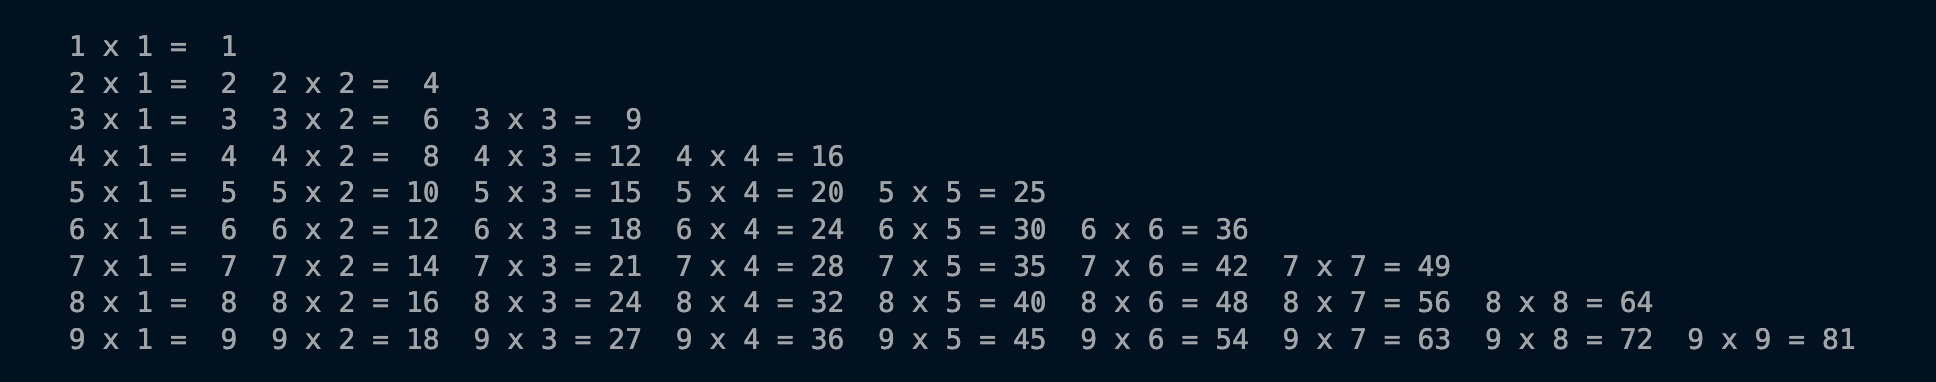
\includegraphics[width=1\linewidth]{Images/99multi.jpg}
            \end{figure}
        \column{0.4\textwidth}
            \begin{figure}
                \centering
                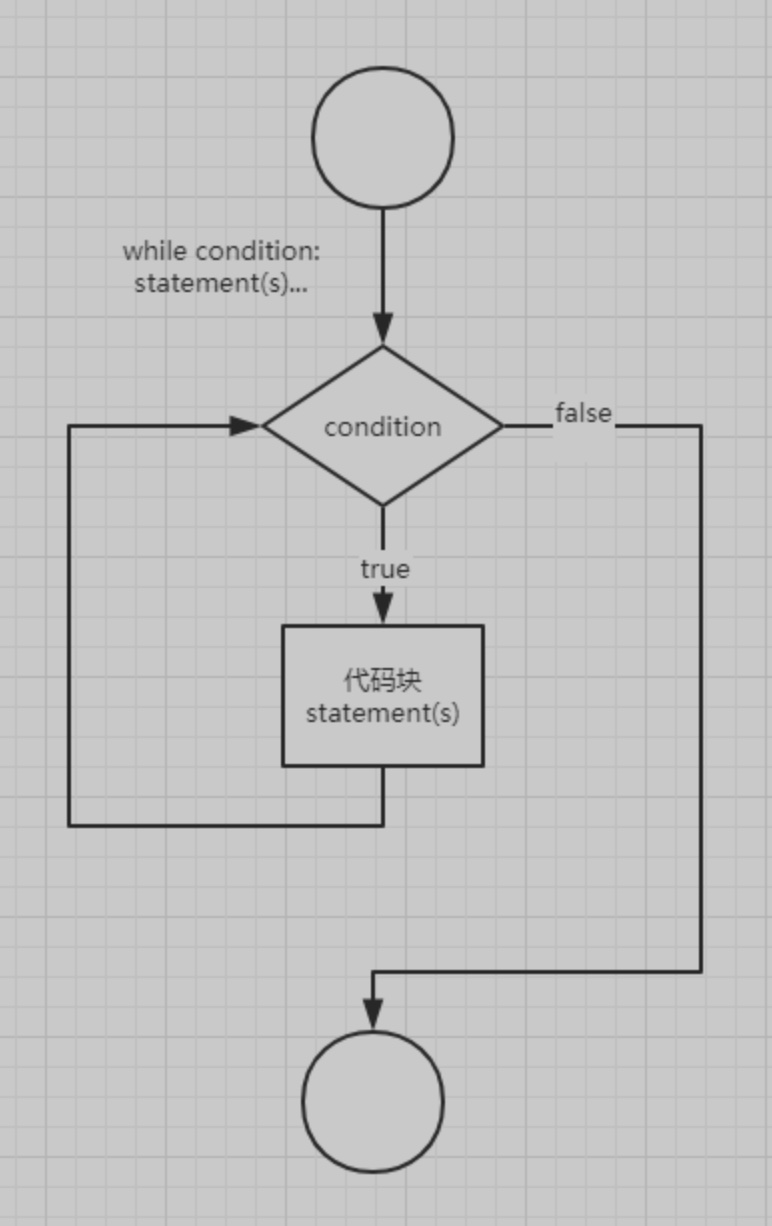
\includegraphics[width=0.7\linewidth]{Images/Loop.jpg}
            \end{figure}
    \end{columns}
\end{frame}
\subsection{函数}
\begin{frame}[standout] 函数 \end{frame}
\begin{frame}[fragile]{函数}
    \begin{columns}
        \column{0.5\textwidth}
        \begin{myoutline}
            \1 定义:
                \2 函数是一种\textcolor{red}{仅在调用时运行}的代码块
                    \3 全局变量(函数外部创建的变量)
                    \3 局部变量(在函数内部被赋值然后使用的变量\dots)
                \2 可以将数据(参数)传递到函数中
                \2 函数可以把数据作为结果返回
            \1 种类:
                \2 内置函数(str(), float(), int()\dots)
                \2 自定义函数
                    \3 无参数, 返回值
                    \3 无参数,有返回值
                    \3 位置参数
                    \3 关键字参数
                    \3 参数数目不确定 *args
                    \3 参数数目不确定 **kwargs
                \2 匿名函数(不推荐, 不易读)
                \2 递归函数(不易读)
                \2 装饰器(了解,用到再讲)
        \end{myoutline}
        \column{0.25\textwidth}
        \begin{lstlisting}
# test1
def myfunc():
    x = 1
    return
print(x)
# test2
X = 1
def myfunc2():
    print(X)
    return
myfunc2()
print(X)
# test3
def myfunc3():
    global S
    S = 3
    return
print(S)
myfunc3()
print(S)

        \end{lstlisting}
        \column{0.25\textwidth}
        \begin{lstlisting}
# test4
def func():
    return

type(func())
a = func()
print(a)
priont(f'{a}')
        \end{lstlisting}
        
    \end{columns}

    
\end{frame}
\subsection{IO操作}
\begin{frame}[standout] IO操作 \end{frame}
\begin{frame}{IO操作-文件打开或创建}
    在 Python 中使用文件的关键函数是 open() 函数。
    open() 函数有两个参数:文件名和模式。
    \begin{myoutline}
        \1 文件名
        \1 模式
            \2 文件打开模式
                \3 r 读取 - \textcolor{red}{默认值}。打开文件进行读取,如果文件不存在则报错。
                \3 a 追加 - 打开供追加的文件,如果不存在则创建该文件。
                \3 w 写入 - 打开文件进行写入,如果文件不存在则创建该文件。
                \3 x 创建 - 创建指定的文件,如果文件存在则返回错误。
            \2 读作文本或二进制
                \3 t 文本 - \textcolor{red}{默认值}。文本模式。
                \3 b 二进制 - 二进制模式(例如图像)。
    \end{myoutline}
\end{frame}

\begin{frame}{IO操作-文件写入和读取}
    \begin{myoutline}
        \1 open() 函数返回文件对象
        \1 写入: 文件对象的 write 方法
        \1 读取: 文件对象的 read 方法用于读取文件的内容
            \2 read() 默认情况下, read() 方法返回整个文本,也可以指定要返回的字符数
            \2 readline() \textcolor{red}{readline() 方法每次}返回一行(iterator)
            \2 readlines() 把文件当做 list 返回,一行为一个元素
    \end{myoutline}


\end{frame}

\begin{frame}[fragile]{IO操作-文件关闭和删除}
    \begin{lstlisting}
import os

os.remove("demofile.txt")  \# 删除文件
os.rmdir("myfolder")  \# 删除文件夹
    \end{lstlisting}
\end{frame}
\subsection{语法糖}
\begin{frame}[standout] 语法糖 \end{frame}
\begin{frame}{语法糖(Syntax Sugar)}
    \tiny{在计算机语言中添加的某种语法,这种语法对语言的功能并没有影响,但更方便程序员使用。简而言之,语法糖让程序更加简洁,有更高的可读性}
    \begin{myoutline}
        \1 连续比较1 < x < 10 (x > 1 and x < 10)
        \1 三元表达式(结果一 if 判断条件 else 结果二)
        \1 列表推导式
        \1 字典推导式
        \1 集合推导式
        \1 迭代器对象(Iterator Object)
            \2 把一个类作为一个迭代器使用需要在类中实现两个方法 \_\_iter\_\_() 与 \_\_next\_\_() 
        \1 生成器函数(Generator Function)(实战项目一会详细演示)(\textcolor{red}{非常重要!})
            \2 在 Python 中,使用了 yield 的函数被称为生成器(generator).
            \2 跟普通函数不同的是,生成器是一个返回迭代器的函数,只能用于迭代操作,更简单点理解生成器就是一个迭代器。
            \2 在调用生成器运行的过程中,每次遇到 yield 时函数会暂停并保存当前所有的运行信息,返回 yield 的值, 并在下一次执行 next() 方法时从当前位置继续运行。
            \2 其实for循环就在调用next方法,next是一个相对底层的方法,for循环基于它
            \2 调用一个生成器函数(Generator Function),返回的是一个迭代器对象(Iterator Object)。
        \1 装饰器(了解)(实战项目中如有时间空余会演示)
        \1 \dots
    \end{myoutline}
\end{frame}

\begin{frame}[standout] Q \& A! \end{frame}
\begin{frame}[standout] Thank you! \end{frame}

\section{第四节 \space Python进阶知识}
\subsection{PyCharm的安装和配置}
\begin{frame}[standout] 第四节 \quad Python 进阶知识 \end{frame}
\begin{frame}[standout] PyCharm的安装 \end{frame}
\begin{frame}[fragile]{PyCharm的安装}
    \begin{myoutline}
        \1 官网 https://www.jetbrains.com/pycharm/
    \end{myoutline}

    \begin{lstlisting}
# macos
brew install --cask pycharm-ce  # 社区版
brew install --cask pycharm  # 专业版
# or 直接官网安装, 不再掩饰

# windows / linux
# 直接官网安装
# 演示!
    \end{lstlisting}
    
\end{frame}

\begin{frame}[fragile]{PyCharm的配置(MacOS为例)}
    \begin{columns}
        \column{0.6\textwidth}
        \begin{lstlisting}
# ---------------------------------
# set outer tools
# Auto PEP8 # conda install autopep8 
# ---------------------------------
Name: AutoPep8
Description: autopep8 your code
Program: autopep8
Arguments: --in-place --aggressive --aggressive $FilePath$
Working directory: $ProjectFileDir$
Output filters: $FILE_PATH$\:$LINE$\:$COLUMN$\:.*
# ---------------------------------
# plugins recommand
# ---------------------------------
# Key Promoter X
# CodeGlance3
# Json Parser
# Rainbow Brackets
# Rainbow CSV
        \end{lstlisting}
        \column{0.4\textwidth}
        \begin{lstlisting}
# ---------------------------------
# 安装专业版并使用学生(教育)邮箱激活一年
# ---------------------------------
# 注册jetbrains账号
# https://account.jetbrains.com/login
# 使用学生或教师邮箱, 免费申请专业版
# https://www.jetbrains.com/shop/eform/students/
# 然后去邮箱里查看, 按照邮件提示操作即可
# 成功后, 下载安装 PyCharm 专业版本, 
# 选择help选项卡 -> registe plugins, 登录账号即可
# ---------------------------------
# 新建一个项目 Project 并运行测试文件
# ---------------------------------
# WSL整合进 PyCharm, 需要专业版
# - 不再演示如何安装 WSL, 如何配置 WSL
# - 查看左下角脚注链接的官方文档
        \end{lstlisting}
    \end{columns}
    \footnotenoindex{http://www.zhaohuanan.cc/category/pycharm.html}
    \footnotenoindex{https://learn.microsoft.com/zh-cn/windows/wsl/}
    \footnotenoindex{https://www.jetbrains.com/help/pycharm/using-wsl-as-a-remote-interpreter.html\#configure-wsl}
\end{frame}



\subsection{模块与包}
\begin{frame}[standout] 模块与包 \end{frame}
\begin{frame}{模块与包的概念}
    \begin{columns}
        \column{0.5\textwidth}
        \begin{myoutline}
            \1 内建对象(Built-in Bbjects)
                \2 print(), str()
                \2 int, str, float
                \2 dir(\_\_builtins\_\_) 
            \1 模块(Module)
                \2 需要import导入
                \2 使用 Python 编写的模块.py
                \2 使用 C 编写的动态加载模块(.dll, .pyd, .so, .sl等)
                \2 内建的 C 编写的模块 sys.builtin\_module\_names
            \1 包(Package)
                \2 需要import导入
                \2 可包含子模块或递归地包含子包的 Python \textcolor{red}{模块}
                \2 从技术上说,包是带有 \_\_path\_\_ 属性的 Python 模块。
                \2 简单来说,它更像是一个文件夹。
        \end{myoutline}
        \column{0.5\textwidth}
        \begin{myoutline}
            \1 标准库(Standard Library)
                \2 标准库相当于解释器的外部扩展,在我们安装 python 解释器的时候,就一块安装上了。
                \2 它并不会随着解释器的启动而启动(builtins),要想使用这些外部扩展,必须提前导入(os)。
                \2 os, sys, time等这些内置模块的的集合
            \1 第三模块,包
        %         \2 使用pip, conda等安装的网上发布的Python 扩展包或者其他语言比如 C, Rust写的扩展包
        %         \2 演示: 寻找第三方包的安装位置
            \1 sys.path
                \2 自定义模块、包——需要先放到python环境变量(sys.path)目录下后 再导入
        \end{myoutline}
    \end{columns}
\end{frame}

\begin{frame}[fragile]{演示}
    \begin{columns}
        \column{0.5\textwidth}
        \begin{myoutline}
            \1 安装一个第三方包, 如 pandas, matplotlib
                \2 导入包, 并演示功能
                \2 ctr/cmd 鼠标点击包名进入包源代码中
            \1 自己创建一个自定义模块
                \2 导入模块中的函数, 并演示功能
                \2 \_\_name\_\_变量
                    \3 运行本文件则为\_\_name\_\_
                    \3 在别的 py 文件中导入后运行则为模块名!
                \2 \_\_pycache\_\_
                    \3  python mymodule.cpython-39.pyc
        \end{myoutline}
        \column{0.5\textwidth}
        \begin{lstlisting}
def myprint():
    print("我在我的模块里!")
    print(__name__)


if __name__ == "__main__":
    myprint()
# myprint()
        \end{lstlisting}
    \end{columns}
\end{frame}



\subsection{异常处理}
\begin{frame}[standout] 异常处理 \end{frame}
\begin{frame}{异常处理}
    \tiny{为了保持大型程序的健壮和稳定,python提供了非常重要的三个功能特性来处理python程序在运行中出现的异常和错误。你可以使用该功能来调试python程序。}

    \begin{myoutline}
        \1 异常处理
            \2 try except的关键字
                \3 try 后跟正常逻辑
                \3 except 捕捉错误信息
                \3 else 如果 except 中描述的错误没捕捉到,就会执行(可选)
                \3 finally 不论是否捕捉到错误,注定执行(可选)
            \2 import builtins; print(dir(builtins))
                \3 官方文档
                \3 https://www.runoob.com/python/python-exceptions.html
        \1 触发异常
            \2 raise函数: Python 允许程序自行引发异常,使用 raise 语句即可
        \1 断言(Assertions)
            \2 assert True     \# 条件为 true 正常执行
            \2 assert False    \# 条件为 false 触发异常
        \1 演示(以打开不存在的文件为例)
    \end{myoutline}
\end{frame}
\subsection{面向对象编程}
\begin{frame}[standout] 面向对象编程 \end{frame}

\begin{frame}[fragile]{把大象装进冰箱!--函数式编程的问题}
    \begin{lstlisting}
# 把大象装进冰箱!!
a = "大象"
open_ice_door()  # 开冰箱门,需要自己实现开冰箱门的函数
push(a)   # 推大象进入
close_ice_door()  # 关冰箱门,需要自己实现关冰箱门的函数
    \end{lstlisting}
    \footnotenoindex{https://zhuanlan.zhihu.com/p/437925568}
\end{frame}

\begin{frame}[fragile]{把大象装进冰箱!--函数式编程的问题}
    \begin{lstlisting}
# 把大象装进冰箱!!
a = "大象"
open_ice_door()  # 开冰箱门,需要自己实现开冰箱门的函数
push(a)   # 推大象进入
close_ice_door()  # 关冰箱门,需要自己实现关冰箱门的函数

# 那如果是把大象装进洗衣机呢?

a = "大象"
open_washer _door()  # 开洗衣机门,需要自己实现开洗衣机门的函数
push(a)   # 推大象进入
close_washer_door()  # 关洗衣机门,需要自己实现关洗衣机门的函数
    \end{lstlisting}
    \footnotenoindex{https://zhuanlan.zhihu.com/p/437925568}
\end{frame}

\begin{frame}[fragile]{把大象装进冰箱!--函数式编程的问题}
    \begin{lstlisting}
# 把大象装进冰箱!!
a = "大象"
open_ice_door()  # 开冰箱门,需要自己实现开冰箱门的函数
push(a)   # 推大象进入
close_ice_door()  # 关冰箱门,需要自己实现关冰箱门的函数

# 那如果是把大象装进洗衣机呢?

a = "大象"
open_washer _door()  # 开洗衣机门,需要自己实现开洗衣机门的函数
push(a)   # 推大象进入
close_washer_door()  # 关洗衣机门,需要自己实现关洗衣机门的函数

# 那如果是把大象装进铁笼呢?

a = "大象"
open_hot_door()  # 开铁笼门,需要自己实现开铁笼门的函数
push(a)   # 推大象进入
close_hot_door()  # 关铁笼门,需要自己实现关铁笼门的函数
    \end{lstlisting}
    \footnotenoindex{https://zhuanlan.zhihu.com/p/437925568}
\end{frame}

\begin{frame}{万物皆对象}
    \tiny{
        R 是一个函数式编程的语言 (大象装进冰箱的弊端!)

        Java 完全面向对象

        Python 既可以以函数式编程方式写程序, 也可以以面向对象编程方式写程序!

        如果你以前没有接触过面向对象的编程语言, 那你可能需要先了解一些面向对象语言的一些基本特征, 在头脑里头形成一个基本的面向对象的概念, 这样有助于你更容易的学习Python的面向对象编程。
    
        接下来我们先来简单的了解下面向对象的一些基本特征。

        \begin{myoutline}
            \1 对象?
                \2 几只胳膊 (属性, 名词)
                \2 几条腿 (属性, 名词)
                \2 打人, 吃饭 (方法, 动词)
            \1 大象装进?里面(冰箱, 洗机器,铁笼)
                \2 对象都是容器(属性)
                \2 对象都有 open\_door(方法)
                \2 对象都有 close\_door(方法)
                \2 对象都有 push(方法)
        \end{myoutline}
    }
\end{frame}

\begin{frame}{面向对象编程思想}
    \small
    \begin{myoutline}
        \1 类(Class):
            \2 用来描述具有相同的\textcolor{red}{属性}和\textcolor{blue}{方法}的\textcolor{green}{对象}的\textcolor{pink}{集合}
                    \3 \textcolor{green}{A, G, C, T}这四个碱基(对象)都属于\textcolor{pink}{碱基}这个集合(类), 都具有\textcolor{red}{分子量}属性和\textcolor{blue}{互补配对}方法
                    \3 \textcolor{green}{狗,小猫}这两种动物(对象)都属于\textcolor{pink}{动物}这个集合(类), 都具有\textcolor{red}{身高, 体重}属性和\textcolor{blue}{吃饭,睡觉}方法
                    \3 \textcolor{green}{南方人,  北方人}两种人(对象)都属于\textcolor{pink}{中国人}这个集合(类), 都具有\textcolor{red}{身高, 体重}属性和\textcolor{blue}{吃饭,睡觉}方法
                    \3 \textcolor{green}{动物, 人}两种生命体(对象)都属于\textcolor{pink}{生命}这个集合(类), 都具有\textcolor{red}{身高, 体重}属性和\textcolor{blue}{吃饭,睡觉}方法
            \2 它定义了该集合中每个对象所共有的\textcolor{red}{属性}和\textcolor{blue}{方法}
        \1 对象:对象是类的实例; 创建对象的过程叫做\textbf{实例化}
            \2 对象包括两个数据成员(\textcolor{red}{属性})(\textcolor{gray}{类变量}和\textcolor{red}{实例变量})和\textcolor{blue}{方法}
        \1 \textcolor{red}{属性}
            \2 \textcolor{gray}{类变量}:类变量在整个实例化的对象中是公用的
                \3 类变量定义在\textbf{类中且在函数体之外}
                \3 类变量通常不作为实例变量(或者说不作为属性)使用, 只为类的属性和方法的实现服务
            \2 \textcolor{red}{实例变量}:在类的声明中,\textcolor{red}{属性}是用变量来表示的
                \3 这种变量就称为实例变量(\textcolor{red}{属性}),是\textcolor{red}{在类声明的内部但是在类的其他成员方法之外}声明的
        \1 \textcolor{blue}{方法}:类中定义的函数
            \2 方法重写 (继承和多态)
            \2 局部变量:\textcolor{red}{定义在方法中的变量},只作用于当前实例的类
    \end{myoutline}
\end{frame}

\begin{frame}{面向对象编程思想}
    \small
    \begin{myoutline}
        \1 类(Class):
            \2 用来描述具有相同的\textcolor{red}{属性}和\textcolor{blue}{方法}的\textcolor{green}{对象}的\textcolor{pink}{集合}
                    \3 \textcolor{green}{A, G, C, T}这四个碱基(对象)都属于\textcolor{pink}{碱基}这个集合(类), 都具有\textcolor{red}{分子量}属性和\textcolor{blue}{互补配对}方法
                    \3 \textcolor{green}{狗,小猫}这两种动物(对象)都属于\textcolor{pink}{动物}这个集合(类), 都具有\textcolor{red}{身高, 体重}属性和\textcolor{blue}{吃饭,睡觉}方法
                    \3 \textcolor{green}{南方人,  北方人}两种人(对象)都属于\textcolor{pink}{中国人}这个集合(类), 都具有\textcolor{red}{身高, 体重}属性和\textcolor{blue}{吃饭,睡觉}方法
                    \3 \textcolor{green}{动物, 人}两种生命体(对象)都属于\textcolor{pink}{生命}这个集合(类), 都具有\textcolor{red}{身高, 体重}属性和\textcolor{blue}{吃饭,睡觉}方法
            \2 它定义了该集合中每个对象所共有的\textcolor{red}{属性}和\textcolor{blue}{方法}
    \end{myoutline}
\end{frame}

\begin{frame}{面向对象编程思想}
    \small
    \begin{myoutline}
        \1 类(Class):
            \2 用来描述具有相同的\textcolor{red}{属性}和\textcolor{blue}{方法}的\textcolor{green}{对象}的\textcolor{pink}{集合}
                    \3 \textcolor{green}{A, G, C, T}这四个碱基(对象)都属于\textcolor{pink}{碱基}这个集合(类), 都具有\textcolor{red}{分子量}属性和\textcolor{blue}{互补配对}方法
                    \3 \textcolor{green}{狗,小猫}这两种动物(对象)都属于\textcolor{pink}{动物}这个集合(类), 都具有\textcolor{red}{身高, 体重}属性和\textcolor{blue}{吃饭,睡觉}方法
                    \3 \textcolor{green}{南方人,  北方人}两种人(对象)都属于\textcolor{pink}{中国人}这个集合(类), 都具有\textcolor{red}{身高, 体重}属性和\textcolor{blue}{吃饭,睡觉}方法
                    \3 \textcolor{green}{动物, 人}两种生命体(对象)都属于\textcolor{pink}{生命}这个集合(类), 都具有\textcolor{red}{身高, 体重}属性和\textcolor{blue}{吃饭,睡觉}方法
            \2 它定义了该集合中每个对象所共有的\textcolor{red}{属性}和\textcolor{blue}{方法}
        \1 对象:对象是类的实例; 创建对象的过程叫做\textbf{实例化}
            \2 对象包括两个数据成员(\textcolor{red}{属性})(\textcolor{gray}{类变量}和\textcolor{red}{实例变量})和\textcolor{blue}{方法}
    \end{myoutline}
\end{frame}

\begin{frame}{面向对象编程思想}
    \small
    \begin{myoutline}
        \1 类(Class):
            \2 用来描述具有相同的\textcolor{red}{属性}和\textcolor{blue}{方法}的\textcolor{green}{对象}的\textcolor{pink}{集合}
                    \3 \textcolor{green}{A, G, C, T}这四个碱基(对象)都属于\textcolor{pink}{碱基}这个集合(类), 都具有\textcolor{red}{分子量}属性和\textcolor{blue}{互补配对}方法
                    \3 \textcolor{green}{狗,小猫}这两种动物(对象)都属于\textcolor{pink}{动物}这个集合(类), 都具有\textcolor{red}{身高, 体重}属性和\textcolor{blue}{吃饭,睡觉}方法
                    \3 \textcolor{green}{南方人,  北方人}两种人(对象)都属于\textcolor{pink}{中国人}这个集合(类), 都具有\textcolor{red}{身高, 体重}属性和\textcolor{blue}{吃饭,睡觉}方法
                    \3 \textcolor{green}{动物, 人}两种生命体(对象)都属于\textcolor{pink}{生命}这个集合(类), 都具有\textcolor{red}{身高, 体重}属性和\textcolor{blue}{吃饭,睡觉}方法
            \2 它定义了该集合中每个对象所共有的\textcolor{red}{属性}和\textcolor{blue}{方法}
        \1 对象:对象是类的实例; 创建对象的过程叫做\textbf{实例化}
            \2 对象包括两个数据成员(\textcolor{red}{属性})(\textcolor{gray}{类变量}和\textcolor{red}{实例变量})和\textcolor{blue}{方法}
        \1 \textcolor{red}{属性}
            \2 \textcolor{gray}{类变量}:类变量在整个实例化的对象中是公用的
                \3 类变量定义在\textbf{类中且在函数体之外}
                \3 类变量通常不作为实例变量(或者说不作为属性)使用, 只为类的属性和方法的实现服务
            \2 \textcolor{red}{实例变量}:在类的声明中,\textcolor{red}{属性}是用变量来表示的
                \3 这种变量就称为实例变量(\textcolor{red}{属性}),是\textcolor{red}{在类声明的内部但是在类的其他成员方法之外}声明的
    \end{myoutline}
\end{frame}
\begin{frame}{面向对象编程思想}
    \small
    \begin{myoutline}
        \1 类(Class):
            \2 用来描述具有相同的\textcolor{red}{属性}和\textcolor{blue}{方法}的\textcolor{green}{对象}的\textcolor{pink}{集合}
                    \3 \textcolor{green}{A, G, C, T}这四个碱基(对象)都属于\textcolor{pink}{碱基}这个集合(类), 都具有\textcolor{red}{分子量}属性和\textcolor{blue}{互补配对}方法
                    \3 \textcolor{green}{狗,小猫}这两种动物(对象)都属于\textcolor{pink}{动物}这个集合(类), 都具有\textcolor{red}{身高, 体重}属性和\textcolor{blue}{吃饭,睡觉}方法
                    \3 \textcolor{green}{南方人,  北方人}两种人(对象)都属于\textcolor{pink}{中国人}这个集合(类), 都具有\textcolor{red}{身高, 体重}属性和\textcolor{blue}{吃饭,睡觉}方法
                    \3 \textcolor{green}{动物, 人}两种生命体(对象)都属于\textcolor{pink}{生命}这个集合(类), 都具有\textcolor{red}{身高, 体重}属性和\textcolor{blue}{吃饭,睡觉}方法
            \2 它定义了该集合中每个对象所共有的\textcolor{red}{属性}和\textcolor{blue}{方法}
        \1 对象:对象是类的实例; 创建对象的过程叫做\textbf{实例化}
            \2 对象包括两个数据成员(\textcolor{red}{属性})(\textcolor{gray}{类变量}和\textcolor{red}{实例变量})和\textcolor{blue}{方法}
        \1 \textcolor{red}{属性}
            \2 \textcolor{gray}{类变量}:类变量在整个实例化的对象中是公用的
                \3 类变量定义在\textbf{类中且在函数体之外}
                \3 类变量通常不作为实例变量(或者说不作为属性)使用, 只为类的属性和方法的实现服务
            \2 \textcolor{red}{实例变量}:在类的声明中,\textcolor{red}{属性}是用变量来表示的
                \3 这种变量就称为实例变量(\textcolor{red}{属性}),是\textcolor{red}{在类声明的内部但是在类的其他成员方法之外}声明的
        \1 \textcolor{blue}{方法}:类中定义的函数
            \2 方法重写 (继承和多态)
            \2 局部变量:\textcolor{red}{定义在方法中的变量},只作用于当前实例的类
    \end{myoutline}
\end{frame}
\begin{frame}[fragile]{把大象装进冰箱!--OOP,伪代码}
    \begin{columns}
        \column{0.5\textwidth}
        \begin{lstlisting}
class Box():
    """盒子类,实现了开门、关门方法"""

    def open_door(self):
        pass

    def close_door(self):
        pass

class IceBox(Box):
    """冰箱"""

    def ice(self):
        """制冷"""
        pass

class WaterBox(Box):
    """洗衣机"""
    
    def add_water(self):
        """加水"""
            pass
        \end{lstlisting}
        \column{0.5\textwidth}
        \begin{lstlisting}
    def sub_water(self):
        """排水"""
        pass   

    def wash(self):
        """洗涤"""
        pass

a = "大象"
ice_box = IceBox()   # 冰箱对象
ice_box.open_door()  # 通知冰箱开门
push(a)   # 推大象进入
ice_box.close_door()  # 通知冰箱关门


# 那我想关老虎呢?
b = "老虎"
ice_box.open_door()  # 通知冰箱开门
push(b)   # 推老虎进入
ice_box.close_door()  # 通知冰箱关门
            \end{lstlisting}
    \end{columns}

\end{frame}

\begin{frame}[standout]{创建类-以碱基互补配对为例}
    \begin{myoutline}
        \1 Class: BioBase(大驼峰命名法)
        \1 实现\_\_init\_\_()方法(接受碱基类型, 分子量)
        \1 实现属性
            \2 碱基
            \2 分子量
        \1 实现方法
            \2 获取碱基
            \2 获取分子量
            \2 获取互补配对的碱基
            \2 设置分子量
        \1 实例化
        \1 类变量(互补配对 dict)
        \1 实例变量(分子量)

    \end{myoutline}
\end{frame}





% class Employee:
%    '所有员工的基类'
%    empCount = 0
 
%    def __init__(self, name, salary):
%       self.name = name
%       self.salary = salary
%       Employee.empCount += 1
   
%    def displayCount(self):
%      print "Total Employee %d" % Employee.empCount
 
%    def displayEmployee(self):
%       print "Name : ", self.name,  ", Salary: ", self.salary


% empCount 变量是一个类变量,它的值将在这个类的所有实例之间共享。你可以在内部类或外部类使用 Employee.empCount 访问。

% 第一种方法__init__()方法是一种特殊的方法,被称为类的构造函数或初始化方法,当创建了这个类的实例时就会调用该方法

% self 代表类的实例,self 在定义类的方法时是必须有的,虽然在调用时不必传入相应的参数。


% self代表类的实例,而非类
% 类的方法与普通的函数只有一个特别的区别——它们必须有一个额外的第一个参数名称, 按照惯例它的名称是 self。


% class Test:
%     def prt(self):
%         print(self)
%         print(self.__class__)
 
% t = Test()
% t.prt()


% 以上实例执行结果为:

% <__main__.Test instance at 0x10d066878>
% __main__.Test



% 从执行结果可以很明显的看出,self 代表的是类的实例,代表当前对象的地址,而 self.__class__ 则指向类。

% self 不是 python 关键字,我们把他换成 runoob 也是可以正常执行的:


% class Test:
%     def prt(runoob):
%         print(runoob)
%         print(runoob.__class__)
 
% t = Test()
% t.prt()


% 以上实例执行结果为:

% <__main__.Test instance at 0x10d066878>
% __main__.Test



% 创建实例对象
% 实例化类其他编程语言中一般用关键字 new,但是在 Python 中并没有这个关键字,类的实例化类似函数调用方式。

% 以下使用类的名称 Employee 来实例化,并通过 __init__ 方法接收参数。

% "创建 Employee 类的第一个对象"
% emp1 = Employee("Zara", 2000)
% "创建 Employee 类的第二个对象"
% emp2 = Employee("Manni", 5000)



% 访问属性
% 您可以使用点号 . 来访问对象的属性。使用如下类的名称访问类变量:

% emp1.displayEmployee()
% emp2.displayEmployee()
% print "Total Employee %d" % Employee.empCount



% Python内置类属性
% __dict__ : 类的属性(包含一个字典,由类的数据属性组成)
% __doc__ :类的文档字符串
% __name__: 类名
% __module__: 类定义所在的模块(类的全名是'__main__.className',如果类位于一个导入模块mymod中,那么className.__module__ 等于 mymod)
% __bases__ : 类的所有父类构成元素(包含了一个由所有父类组成的元组)
% Python内置类属性调用实例如下:


% class Employee:
%    '所有员工的基类'
%    empCount = 0
 
%    def __init__(self, name, salary):
%       self.name = name
%       self.salary = salary
%       Employee.empCount += 1
   
%    def displayCount(self):
%      print "Total Employee %d" % Employee.empCount
 
%    def displayEmployee(self):
%       print "Name : ", self.name,  ", Salary: ", self.salary
 
% print "Employee.__doc__:", Employee.__doc__
% print "Employee.__name__:", Employee.__name__
% print "Employee.__module__:", Employee.__module__
% print "Employee.__bases__:", Employee.__bases__
% print "Employee.__dict__:", Employee.__dict__





% 类的继承
% 面向对象的编程带来的主要好处之一是代码的重用,实现这种重用的方法之一是通过继承机制。

% 通过继承创建的新类称为子类或派生类,被继承的类称为基类、父类或超类。

% 继承语法

% class 派生类名(基类名)
%     ...
% 在python中继承中的一些特点:

% 1、如果在子类中需要父类的构造方法就需要显式的调用父类的构造方法,或者不重写父类的构造方法。详细说明可查看: python 子类继承父类构造函数说明。
% 2、在调用基类的方法时,需要加上基类的类名前缀,且需要带上 self 参数变量。区别在于类中调用普通函数时并不需要带上 self 参数
% 3、Python 总是首先查找对应类型的方法,如果它不能在派生类中找到对应的方法,它才开始到基类中逐个查找。(先在本类中查找调用的方法,找不到才去基类中找)。
% 如果在继承元组中列了一个以上的类,那么它就被称作"多重继承" 。

% 语法:

% 派生类的声明,与他们的父类类似,继承的基类列表跟在类名之后,如下所示:

% class SubClassName (ParentClass1[, ParentClass2, ...]):
%     ...
% 实例
% #!/usr/bin/python
% # -*- coding: UTF-8 -*-
 
% class Parent:        # 定义父类
%    parentAttr = 100
%    def __init__(self):
%       print "调用父类构造函数"
 
%    def parentMethod(self):
%       print '调用父类方法'
 
%    def setAttr(self, attr):
%       Parent.parentAttr = attr
 
%    def getAttr(self):
%       print "父类属性 :", Parent.parentAttr
 
% class Child(Parent): # 定义子类
%    def __init__(self):
%       print "调用子类构造方法"
 
%    def childMethod(self):
%       print '调用子类方法'
 
% c = Child()          # 实例化子类
% c.childMethod()      # 调用子类的方法
% c.parentMethod()     # 调用父类方法
% c.setAttr(200)       # 再次调用父类的方法 - 设置属性值
% c.getAttr()          # 再次调用父类的方法 - 获取属性值
% 以上代码执行结果如下:

% 调用子类构造方法
% 调用子类方法
% 调用父类方法
% 父类属性 : 200
% 你可以继承多个类

% class A:        # 定义类 A
% .....

% class B:         # 定义类 B
% .....

% class C(A, B):   # 继承类 A 和 B
% .....
% 你可以使用issubclass()或者isinstance()方法来检测。

% issubclass() - 布尔函数判断一个类是另一个类的子类或者子孙类,语法:issubclass(sub,sup)
% isinstance(obj, Class) 布尔函数如果obj是Class类的实例对象或者是一个Class子类的实例对象则返回true。
% 方法重写
% 如果你的父类方法的功能不能满足你的需求,你可以在子类重写你父类的方法:

% 实例:

% 实例
% #!/usr/bin/python
% # -*- coding: UTF-8 -*-
 
% class Parent:        # 定义父类
%    def myMethod(self):
%       print '调用父类方法'
 
% class Child(Parent): # 定义子类
%    def myMethod(self):
%       print '调用子类方法'
 
% c = Child()          # 子类实例
% c.myMethod()         # 子类调用重写方法
% 执行以上代码输出结果如下:

% 调用子类方法
% 基础重载方法
% 下表列出了一些通用的功能,你可以在自己的类重写:

% 序号	方法, 描述 & 简单的调用
% 1	__init__ ( self [,args...] )
% 构造函数
% 简单的调用方法: obj = className(args)
% 2	__del__( self )
% 析构方法, 删除一个对象
% 简单的调用方法 : del obj
% 3	__repr__( self )
% 转化为供解释器读取的形式
% 简单的调用方法 : repr(obj)
% 4	__str__( self )
% 用于将值转化为适于人阅读的形式
% 简单的调用方法 : str(obj)
% 5	__cmp__ ( self, x )
% 对象比较
% 简单的调用方法 : cmp(obj, x)
% 运算符重载
% Python同样支持运算符重载,实例如下:

% 实例
% #!/usr/bin/python
 
% class Vector:
%    def __init__(self, a, b):
%       self.a = a
%       self.b = b
 
%    def __str__(self):
%       return 'Vector (%d, %d)' % (self.a, self.b)
   
%    def __add__(self,other):
%       return Vector(self.a + other.a, self.b + other.b)
 
% v1 = Vector(2,10)
% v2 = Vector(5,-2)
% print v1 + v2
% 以上代码执行结果如下所示:

% Vector(7,8)
% 类属性与方法
% 类的私有属性
% __private_attrs:两个下划线开头,声明该属性为私有,不能在类的外部被使用或直接访问。在类内部的方法中使用时 self.__private_attrs。

% 类的方法
% 在类的内部,使用 def 关键字可以为类定义一个方法,与一般函数定义不同,类方法必须包含参数 self,且为第一个参数

% 类的私有方法
% __private_method:两个下划线开头,声明该方法为私有方法,不能在类的外部调用。在类的内部调用 self.__private_methods

% 实例
% #!/usr/bin/python
% # -*- coding: UTF-8 -*-
 
% class JustCounter:
%     __secretCount = 0  # 私有变量
%     publicCount = 0    # 公开变量
 
%     def count(self):
%         self.__secretCount += 1
%         self.publicCount += 1
%         print self.__secretCount
 
% counter = JustCounter()
% counter.count()
% counter.count()
% print counter.publicCount
% print counter.__secretCount  # 报错,实例不能访问私有变量
% Python 通过改变名称来包含类名:

% 1
% 2
% 2
% Traceback (most recent call last):
%   File "test.py", line 17, in <module>
%     print counter.__secretCount  # 报错,实例不能访问私有变量
% AttributeError: JustCounter instance has no attribute '__secretCount'
% Python不允许实例化的类访问私有数据,但你可以使用 object._className__attrName( 对象名._类名__私有属性名 )访问属性,参考以下实例:

% #!/usr/bin/python
% # -*- coding: UTF-8 -*-

% class Runoob:
%     __site = "www.runoob.com"

% runoob = Runoob()
% print runoob._Runoob__site
% 执行以上代码,执行结果如下:

% www.runoob.com
% 单下划线、双下划线、头尾双下划线说明:
% __foo__: 定义的是特殊方法,一般是系统定义名字 ,类似 __init__() 之类的。

% _foo: 以单下划线开头的表示的是 protected 类型的变量,即保护类型只能允许其本身与子类进行访问,不能用于 from module import *

% __foo: 双下划线的表示的是私有类型(private)的变量, 只能是允许这个类本身进行访问了。
\subsection{继承和多态}
\begin{frame}[standout] 继承和多态 \end{frame}
\begin{frame}[fragile]{把大象装进冰箱!--OOP,伪代码}
    \begin{columns}
        \column{0.5\textwidth}
        \begin{lstlisting}
class Box():
    """盒子类,实现了开门、关门方法"""

    def open_door(self):
        pass

    def close_door(self):
        pass

class IceBox(Box):
    """冰箱"""

    def ice(self):
        """制冷"""
        pass

class WaterBox(Box):
    """洗衣机"""
    
    def add_water(self):
        """加水"""
            pass
        \end{lstlisting}
        \column{0.5\textwidth}
        \begin{lstlisting}
    def sub_water(self):
        """排水"""
        pass   

    def wash(self):
        """洗涤"""
        pass

a = "大象"
ice_box = IceBox()   # 冰箱对象
ice_box.open_door()  # 通知冰箱开门
push(a)   # 推大象进入
ice_box.close_door()  # 通知冰箱关门


# 那我想关老虎呢?
b = "老虎"
ice_box.open_door()  # 通知冰箱开门
push(b)   # 推老虎进入
ice_box.close_door()  # 通知冰箱关门
            \end{lstlisting}
    \end{columns}
\end{frame}
% \2 方法重写
% \2 继承: 即一个派生类(derived class)继承基类(base class)的字段和方法。
% 继承也允许把一个派生类的对象作为一个基类对象对待。例如, 有这样一个设计: 一个Dog类型的对象派生自Animal类

% \1 继承: 即一个派生类(derived class)继承基类(base class)的字段和方法。
% \2 继承也允许把一个派生类的对象作为一个基类对象对待。
%     \3 例如, 有这样一个设计: 一个Animal类型的对象派生自Life类

% 多态
\subsection{代码规范}
\begin{frame}[standout] 代码规范 \end{frame}
\begin{frame}[fragile]{PEP8规范(常用的列举)}
    \begin{myoutline}
        \1 代码布局
            \2 每个缩进级别使用4个空格;连续行使用垂直对齐或者使用悬挂式缩进(额外的4个空格缩进)
            \2 空格是首选的缩进方法
            \2 每行最多79个字符
            \2 二元运算符前后换行都允许,只要代码保持一致就行。对于新代码建议在\textcolor{red}{二元运算符前进行换行}
            \2 空白行:使用\textcolor{red}{两个空白行}分隔\textcolor{red}{顶层函数和类定义};\textcolor{red}{类方法定义使用一个空行}分隔;使用额外的空白行来分隔相关逻辑功能
            \2 文件应该使用UTF-8编码, 且不应该有\textcolor{red}{编码声明}
            \2 导入多个库函数应该分开依次导入;导入总是放在文件的顶部,在任何\textcolor{red}{模块注释和文档字符串之后},在模块全局变量和常量之前;导入应按以下顺序进行:标准库导入、有关的第三方库进口、本地应用程序/库特定的导入,每组导入直接用空行分隔;避免通配符导入(import \*)
        \1 字符串
            \2 单引号字符串和双引号字符串相同,代码保持一致即可
            \2 对于三引号字符串,\textcolor{red}{常用三个双引号作文档字符串},文档字符串常用在模块的开端用以说明模块的基本功能,或紧跟函数定义的后面用以说明函数的基本功能
        \1 空格
            \2 避免使用无关的空格,包括空格内、逗号分号前面等; 避免在行末使用空格
            \2 二元运算符在两侧使用一个空格
            \2 当用于指示\textcolor{red}{关键字参数或默认参数值}时,不要在=符号周围使用空格
    \end{myoutline}
    \footnotenoindex{https://www.cnblogs.com/tangjielin/p/16511066.html}
    \footnotenoindex{https://peps.python.org/pep-0008/}
\end{frame}

\begin{frame}[fragile]{PEP8规范(常用的列举)}
    \begin{myoutline}
        \1 使用尾部逗号(trailing commas)
            \2 尾部逗号通常可选,除了用来说明是只有一个元素的元组tuple时
            \2 当参数、值等列表期望经常扩展时,通常是每个值一行,再加上一个尾部逗号
        \1 注释
            \2 代码更改时,相应的注释也要随之高优更改
            \2 注释应该是\textcolor{red}{完整的语句},第一个单词应该大写,除非它是特定标识符
            \2 \textcolor{red}{块注释}:缩进到与该代码相同的级别。块注释的每一行都以#和一个空格开始
            \2 \textcolor{red}{行注释}:对某一语句行进行注释,注释应该与语句至少隔开\textcolor{red}{两个空格},用#和一个空格开始
            \2 对于公共的modules, functions, classes, and methods,需要写文档字符串
            \2 注释应该是完整的语句,第一个单词应该大写,除非它是特定标识符
        \1 命名约定
            \2 python命名规范有点混乱,很难完全保存一致。对于新模块和包,应该遵守这些新的约定,已存在的库内部一致性更重要
            \2 命名应该\textcolor{red}{反应其用途而非实现}
            \2 不要将字符l(小写字母l),O(大写字母o)或I(大写字母I)作为单个字符变量名称
            \2 \textcolor{red}{模块名应该使用简短、全小写}的名字
            \2 \textcolor{red}{类的命名采用大驼峰命名法},即每个单词的首字母大写
            \2 \textcolor{red}{函数名称应该是小写的,为了提高可读性,必须使用由下划线分隔的单词}
    \end{myoutline}
    \footnotenoindex{https://www.cnblogs.com/tangjielin/p/16511066.html}
    \footnotenoindex{https://peps.python.org/pep-0008/}
    \footnotenoindex{https://google.github.io/styleguide/pyguide.html}
\end{frame}
\begin{frame}[fragile]{Google Python命名规范(常用的列举)}
    \begin{myoutline}
        \1 命名
            \2 异常名: ExceptionName ;
            \2 函数名: function\_name ;
            \2 全局常量名: GLOBAL\_CONSTANT\_NAME ;
            \2 全局变量名: global\_var\_name ;
            \2 实例名: instance\_var\_name ;
            \2 函数参数名: function\_parameter\_name ;
            \2 局部变量名: local\_var\_name .
            \2 函数名,变量名和文件名应该是描述性的,尽量避免缩写,特别要避免使用非项目人员不清楚难以理解的缩写,不要通过删除单词中的字母来进行缩写. 始终使用 .py 作为文件后缀名,不要用破折号.
        \1 命名约定
            \2 所谓”内部(Internal)”表示仅模块内可用, 或者, 在类内是保护或私有的。
            \2 用单下划线(\_)开头表示模块变量或函数是protected的(使用from module import \*时不会包含)。
            \2 用双下划线(\_\_)开头的实例变量或方法表示类内私有。
            \2 将相关的类和顶级函数放在同一个模块里. 不像Java, 没必要限制一个类一个模块.对类名使用大写字母开头的单词(如CapWords, 即Pascal风格), 但是模块名应该用小写加下划线的方式(如lower\_with\_under.py). 尽管已经有很多现存的模块使用类似于CapWords.py这样的命名, 但现在已经不鼓励这样做, 因为如果模块名碰巧和类名一致, 这会让人困扰。
    \end{myoutline}
    \footnotenoindex{https://google.github.io/styleguide/pyguide.html}
\end{frame}

\begin{frame}[fragile]{Google Python命名规范(常用的列举)}
    \begin{columns}
        \column{0.6\textwidth}
        \begin{myoutline}
            \1 `\_\_main\_\_'和main()
                \2 即使是一个打算被用作脚本的文件, 也应该是可导入的. 并且简单的导入不应该导致这个脚本的主功能(main functionality)被执行, 这是一种副作用. 主功能应该放在一个main()函数中.
                \2 在Python中, pydoc以及单元测试要求模块必须是可导入的. 你的代码应该在执行主程序前总是检查 if \_\_name\_\_ == `\_\_main\_\_' , 这样当模块被导入时主程序就不会被执行.
                \2 若使用 absl, 请使用 app.run\dots 所有的顶级代码在模块导入时都会被执行. 要小心不要去调用函数, 创建对象, 或者执行那些不应该在使用pydoc时执行的操作.
        \end{myoutline}
        \column{0.3\textwidth}
        \begin{lstlisting}
from absl import app 
... 
def main(argv): 
    # process non-flag arguments
    ... 


if __name__ == '__main__': 
    app.run(main)

# 否则,使用:
def main():
    ... 


if __name__ == '__main__': 
    main()
        \end{lstlisting}
    \end{columns}
    \footnotenoindex{https://google.github.io/styleguide/pyguide.html}
\end{frame}

\begin{frame}[fragile]{Google Python命名规范(常用的列举)}
    \begin{myoutline}
        \1 类型注释
            \2 通用规则请先熟悉下PEP-484对于方法
            \2 仅在必要时才对 self 或 cls 注释(实战课三当中进行讲解)
            \2 若对类型没有任何显示, 请使用 Any
            \2 无需注释模块中的所有函数
            \2 公共的API需要注释
            \2 在代码的安全性,清晰性和灵活性上进行权衡是否注释
            \2 对于容易出现类型相关的错误的代码进行注释
            \2 难以理解的代码请进行注释
            \2 若代码中的类型已经稳定,可以进行注释
            \2 对于一份成熟的代码,多数情况下,即使注释了所有的函数,也不会丧失太多的灵活性.
    \end{myoutline}
    \footnotenoindex{https://google.github.io/styleguide/pyguide.html}
\end{frame}
\subsection{补充知识}
\begin{frame}[standout] 补充知识 \end{frame}
\begin{frame}{补充知识}
    \begin{myoutline}
        \1 下划线的 6 个作用
            \2 用在 Python 解释器,表示上一次的执行结果
            \2 代码中一个独立的下划线,表示这个变量不重要
            \2 类的内部,双下划线作为变量名或函数名的开头,表示私有
            \2 双下划线开头和结尾的方法,是魔术方法
                \3 比如常见的 `\_\_init\_\_', `\_\_dict\_\_', `\_\_dir\_\_', `\_\_doc\_\_', `\_\_eq\_\_' 等等
            \2 作为变量名中间的一部分
            \2 作为数字中间的一部分,更易读
    \end{myoutline}
\end{frame}
\begin{frame}{补充知识}
    \begin{myoutline}
        \1 Jupyterlab扔后台?conda/brew/apt install tmux
        \1 使用服务器的Jupyterlab
        \1 服务器(没有root权限)上安装的jupyterlab 后 自动加载的网页里不能显示notebook是啥(IP原因)
    \end{myoutline}
\end{frame}
\begin{frame}[fragile]{补充知识}
    \begin{myoutline}
        \1 Windows 配置 scoop 及 scoop 安装软件和命令
            \2 直接演示
    \end{myoutline}
    \begin{lstlisting}
# 进入powershell
set-alias ll  # ls
# 步骤 1:在 PowerShell 中打开远程权限
Set-ExecutionPolicy RemoteSigned -scope CurrentUser;
cd ~
# 步骤 2: 自定义 Scoop 安装目录
# 如果跳过该步骤, Scoop 将默认把所有用户安装的 App 和 Scoop 
# 本身置于C:\Users\user_name\scoop
# C:\Users\vagrant
mkdir scoop
$env:SCOOP='C:\Users\vagrant\scoop'
[Environment]::SetEnvironmentVariable('SCOOP', $env:SCOOP, 'User')

# 步骤 3:下载并安装 Scoop
iwr -useb https://gitee.com/glsnames/scoop-installer/raw/master/bin/install.ps1 | iex
scoop config SCOOP_REPO 'https://gitee.com/glsnames/scoop-installer'  # 设置镜像(如果软件安装失败的话)
scoop install git  # 必须的依赖项
    \end{lstlisting}

\end{frame}
\begin{frame}[fragile]{补充知识}
    \begin{lstlisting}
# step1: 添加官方维护的extras库(含大量GUI程序)
# 国内源 scoop bucket add extras https://gitee.com/scoop-bucket/extras.git
scoop bucket add extras
# step2 更新源
scoop update
# step3 安装 App和命令行工具(必装工具, conda装好可以不再装了)
scoop install git
scoop install miniconda3  # 安装全完全卸载原来安装的 miniconda!
scoop install sudo  # 调用管理员权限
scooop install tldr  # too long dont read!
# (类 unix 完美,windows 能用但信息提供的是类 unix 的,对 windows 不一定能够完全适用)
# 类unix 可以conda install tldr
scoop install busybox  # 项目实战一会用到! zcat命令的依赖
scoop install cwrsync  # 项目实战一会用到!
scoop install windows-terminal
scoop install powertoys


# 管理:
scoop list  # 查看已安装程序
scoop status  # 查看更新
scoop cleanup  # 删除旧版本
scoop checkup  # 自身诊断
    \end{lstlisting}
\end{frame}

\begin{frame}[standout] Q \& A! \end{frame}
\begin{frame}[standout] Thank you! \end{frame}


\section{项目实战一 FASTA与FASTQ}
\subsection{项目一 序列文件的处理}

\begin{frame}[standout] 项目一 \quad 序列文件的处理 \end{frame}

\begin{frame}[standout] 序列储存格式的介绍 \end{frame}
\begin{frame}[fragile]{序列储存格式的介绍--FASTA 文件格式}
    \begin{columns}
        \column{0.5\textwidth}
        \begin{myoutline}
            \1 FASTA格式
                \2 一种用于表示核苷酸序列或多肽序列的文本格式;其中碱基对或氨基酸用单个字母来表示
                \2 允许在序列前添加序列名及注释
                \2 该格式已成为生物信息学领域的一项标准
            \1 FASTA文件各行记录信息如下:
                \2 第一行
                    \3 由大于号">"开头的任意文字说明,用于序列标记
                    \3 为了保证后续分析软件能够区分每条序列,\textcolor{red}{单个序列的标识必须是唯一的}
                \2 第二行
                    \3 序列本身; 只允许使用既定的核苷酸或氨基酸编码符号。
                    \3 通常核苷酸符号大小写均可, 而氨基酸常用大写字母。
                    \3 注意有些程序对大小写有明确要求。一般每行60-80个字母。
        \end{myoutline}
        \column{0.45\textwidth}
        \begin{lstlisting}
>HWI-D00433:463:HNT7JBCXX:1:1101:19071:2193 1:N:0:TTCTCCAT
CCTACGGGACGCATCAGTGAGGAATATTGGTCAATGGACGCGAGTCTGAACCAGCCAAGT
AGCGTGAAGGATGAAGGCCCGATGGGTTGTAAACCTCTTTTATCTGGGAATAAAACGTGC
CACGTGTGGTATTTTGTATGTACCATAAGAATAAGTATCGGCTAACTCCGTGCCAGCAGC
CGCGGTAATACGGAGGATCCGAGCGTTATCCGGATTTATTGGGTTTAAAGGGTGCGCAGG
CGGTCTGTTA
>HWI-D00433:463:HNT7JBCXX:1:1101:1713:2316 1:N:0:TTCTCCAT
CCTACGGGGTTCACCAGTAGGGAATCTTCCACAATGGGCGAAAGCCTGATTGAGCAAAGC
CGCGTGTTTTAAGAAGGTCTTCGGATCGTAAAACCCTGTTGTTAGAGAAGAAAGTGCGTG
CGCGTAACTGTTCACGTTTCTACTGTATCTAACAAGAAAGCACCGGCTAACTACGTTCCA
        \end{lstlisting}
    \end{columns}
    \footnotenoindex{https://zhuanlan.zhihu.com/p/363971040}
\end{frame}

\begin{frame}[fragile]{序列储存格式的介绍--FASTA 文件格式}
    \begin{lstlisting}
# legend server
cd /home/zhaohuanan/3.project/2022_Other_projects/2022-09-25_Prepared_data/FASTA
rsync -avzP rsync://hgdownload.cse.ucsc.edu/goldenPath/mm39/chromosomes/ .
# check一下md5
md5sum -c md5sum.txt

(base) PS C:\Users\vagrant\PythonForBioinformatics> rsync -avzP rsync://hgdownload.cse.
ucsc.edu/goldenPath/mm39/chromosomes/chrM.fa.gz .
receiving incremental file list
chrM.fa.gz
          5,385 100%    5.14MB/s    0:00:00 (xfr#1, to-chk=0/1)

sent 43 bytes  received 5,492 bytes  299.19 bytes/sec
total size is 5,385  speedup is 0.97

# 接下来我们需要将genome生成一下,未确定的基因组区域暂不考虑,只看确定的基因组
# 测试命令
echo `seq 1 1 19` X Y M | awk 'BEGIN {printf "cat "}{for(i=1; i<=NF;i++){printf "chr"$i".fa.gz "}}'
# 写入genome文件
echo `seq 1 1 19` X Y M | awk 'BEGIN {printf "cat "}{for(i=1; i<=NF;i++){printf "chr"$i".fa.gz "}}' | \
    sh > genome_ucsc_mm39.fa.gz
zcat genome_ucsc_mm39.fa.gz | grep -v N | less # linux/window
zcat < genome_ucsc_mm39.fa.gz | grep -v N | less # macos
    \end{lstlisting}
\end{frame}


\begin{frame}[fragile]{序列储存格式的介绍--FASTQ 文件格式}
    \begin{myoutline}
        \1 第一行
            \2 以@开头
            \2 后面是reads的ID以及其他信息
            \2 例如下一页例中 HWUSI-EAS100R代表Illumina设备名称,
            \2 6代表flowcell中的第六个lane,73代表第六个lane中的第73个tile
            \2 941:1973代表该read在该tile中的x:y坐标信息;
            \2 \#0, 若为多样本的混合作为输入样本,则该标志代表样本的编号,用来区分个样本中的reads/
            \2 /1代表paired end中的前一个read。
        \1 第二行
            \2 read的序列
            \2 紧接着下面两行代表该read的质量
        \1 第三行
            \2 以“+”开头,跟随着该read的名称(一般于@后面的内容相同),但有时可以省略,但“+”一定不能省
    \end{myoutline}
    \footnotenoindex{https://baike.baidu.com/item/fastQ格式 (rmspace)}
\end{frame}
\begin{frame}[fragile]{序列储存格式的介绍--FASTQ 文件格式}
    \begin{myoutline}
        \1 第四行
        \2 代表reads的质量。这一行可以详细说一下!
        \2 Illumina测序仪是按照荧光信号来判断所测序的碱基是哪一种的,例如红黄蓝绿分别对应ATCG,那么一旦出现一个紫色的信号该怎么判断呢?
        \2 因此对每个结果都有一个概率的问题。起初sanger中心用Phred quality score来衡量该read中每个碱基的质量,既-10lgP \#(lg意为log10)
            \3 其中P代表该碱基被测序错误的概率
            \3 如果该碱基测序出错的概率为0.001, 则Q应该为30,那么30+33=63,那么63对应的ASCii码为`?',则在第四行中该碱基对应的质量代表值即为`?'
            \3 ASCII https://baike.baidu.com/item/ASCII
    \end{myoutline}
    \begin{lstlisting}
@SEQ_ID
GATTTGGGGTTCAAAGCAGTATCGATCAAATAGTAAATCCATTTGTTCAACTCACAGTTT
+
!''*((((***+))%%%++)(%%%%).1***-+*''))**55CCF

# 例如在NCBI看到的FASTQ格式如下
@HWUSI-EAS100R:6:73:941:1973#0/1
GATTTGGGGTTCAAAGCAGTATCGATCAAATAGTAAATCCATTTGTTCAACTCACAGTT
+HWUSI-EAS100R:6:73:941:1973#0/1
!''*((((***+))%%%++)(%%%%).1***-+*''))**55CCF
    \end{lstlisting}
\end{frame}

\begin{frame}[fragile]{序列储存格式的介绍--FASTQ 文件格式}
    \begin{lstlisting}
# from illumina
@E00591:528:HHVW3CCX2:2:1101:17360:2170 1:N:0:GATCAGCG:ACTA
TGGAGTGAGTACGGTGTGCGTTGAAGTCCTCGTTGTCTTGTTGGCAGGGGTCTGCACCCGGGAGCCCCCGTTCTATATCATCACTGAGATCATGACCTACGGGAACCTCCTCGACTACCTCAGGGAGTGCAACTGCAACGAG
+
JJJJAFFFFJFJJJAFFJJJJFJFFJJFFFJF7A<FJ7JF-<F-7A7<JF7<FJJJ-F<JJJJFJJJJJJ<<AJFJAJJ<7AJFFFJ-<7AFFJJJA-<FF--7FJ-F7-7FA7F<FFJA-7FJJJJF<JF7F7A7-777<-
# from mgi
@Beta12AdemL1C001R00100000184/1
GTGTCCGTATCTTCACCCCACCACAAACTATTAGCTTTAGAAAGGAAAAGAAAAACCACAACAAAACAGTGTGTGTGTACCAAAGACTTATATGTGCATAAGCAAAAGCAAACAATAGCATTAGCAGGAACTCGTGGACATTCCAGGGAA
+
ICIDIIIDEDIDBIEIIIIEIIEIEEEID@DDE4IDDDEID>EIIEEEEIEEEEEIIEIEEIECEEIE4DIDIDDC6DEIIE@E6EI5CBDEDICIIECEEIIAEEEIIDEEIE:CD:IECABIIEI>E8ICI,CI9DIEDCIIE@>HEC
# from sra
@fig7_untreated_rep1.1 1 length=150
TTACAAGACTGNTGTATTAGTTTATACTACAAGGACAGGCCCATTNGNNTNTNTTNTTTTNAANTAGGGANATAGTTGGTATTAGGATTAGNATTGTTGTGAAGTATAGTANGGATGCTACTTGNCCAATGATGGTAAAAGGGTAGCTTA
+fig7_untreated_rep1.1 1 length=150
AFFFFFFFFFF#FFFFFFFFFFFFFFFFFFFFFFFFFFFFFFF/F#F##F#F#FF#FFFF#FF#FFFFFF#FFFFFFFFFFFFFFFFFFFA#FFFFFFFFFFFFFFFFFFF#FFFFFFFFFFFF#A/FFFF/FFFFFFF/FFFFFFFFFF
    \end{lstlisting}
\end{frame}
\subsection{FASTQ文件的操作}
\begin{frame}[standout] FASTQ文件的操作 \end{frame}
\begin{frame}{FASTQ文件的操作}
    \begin{myoutline}
        \1 FASTQ文件的操作
            \2 读取FASTQ文件并以FASTA格式输出
            \2 解析FASTQ的质量值,计算Q30比例
            \2 根据FastQC报告对FASTQ文件进行截取
            \2 根据FastQC报告,过滤低质量的lane,tile数据
    \end{myoutline}
\end{frame}

\subsection{FASTA文件的操作}
\begin{frame}[standout] FASTA文件的操作 \end{frame}
\begin{frame}{FASTA文件的操作}
    \begin{myoutline}
        \1 FASTA文件的操作
             \2 读取FASTA文件,并将其中U替换成T
             \2 读取FASTA文件,并输出反向互补序列
             \2 计算基因组序列的长度
             \2 计算基因组各染色体的平均GC含量
             \2 计算基因组中N的总长度(effective length)
    \end{myoutline}
\end{frame}

% 3. FASTA 文件的操作与计算9月24日 10:00-11:00|未开始

\begin{frame}[fragile]{Docstring-reST}
    % https://queirozf.com/entries/python-docstrings-reference-examples
    \tiny
    \begin{lstlisting}
def func(arg1, arg2):
    """Summary line.

    Extended description of function.

    :param int arg1: Description of arg1.
    :param str arg2: Description of arg2.
    :raise: ValueError if arg1 is equal to arg2
    :return: Description of return value
    :rtype: bool

    :example:

    >>> a=1
    >>> b=2
    >>> func(a,b)
    True
    """

    if arg1 == arg2:
        raise ValueError('arg1 must not be equal to arg2')

    return True
    \end{lstlisting}
\end{frame}

\begin{frame}[fragile]{Docstring-Google Style}
    \tiny
    \begin{columns}
        \column{0.6\textwidth}
        \begin{lstlisting}
def func(arg1, arg2):
    """Summary line.

    Extended description of function.

    Args:
        arg1 (int): Description of arg1
        arg2 (str): Description of arg2

    Returns:
        bool: Description of return value

    Raises:
        AttributeError: The ``Raises`` section is a list of all 
            exceptions that are relevant to the interface.
        ValueError: If `arg2` is equal to `arg1`.

    Examples:
        Examples should be written in doctest format, and should
            illustrate how to use the function.
        >>> a=1
        >>> b=2
        >>> func(a,b)
        True
    """
            \end{lstlisting}
            \column{0.4\textwidth}
            \begin{lstlisting}
    if arg1 == arg2:
        raise ValueError(
            'arg1 must not be equal to arg2'
        )

    return True
            \end{lstlisting}
    \end{columns}

\end{frame}
\begin{frame}[fragile]{Docstring-Numpy Style}
    \tiny
    \begin{columns}
        \column{0.6\textwidth}
        \begin{lstlisting}
def func(arg1, arg2):
    """Summary line.

    Extended description of function.

    Parameters
    ----------
    arg1 : int
        Description of arg1
    arg2 : str
        Description of arg2

    Returns
    -------
    bool
        Description of return value

    Raises
    ------
    AttributeError
        The ``Raises`` section is a list of all exceptions
        that are relevant to the interface.
    """
            \end{lstlisting}
            \column{0.4\textwidth}
            \begin{lstlisting}
    """
    ValueError
        If `arg2` is equal to `arg1`.

    See Also
    --------
    otherfunc: some other related function

    Examples
    --------
    These are written in doctest format, and should illustrate how to
    use the function.

    >>> a=1
    >>> b=2
    >>> func(a,b)
    True
    """

    if arg1 == arg2:
        raise ValueError(
            'arg1 must not be equal to arg2'
        )
    return True
            \end{lstlisting}
    \end{columns}

\end{frame}
\begin{frame}[standout] Q \& A! \end{frame}
\begin{frame}[standout] Thank you! \end{frame}

\section{项目实战三 基因注释文件处理}
\subsection{项目三 基因注释文件处理}

\begin{frame}[standout] 项目三 \quad 基因注释文件处理 \end{frame}

\begin{frame}[standout] 基因注释与GTF和GFF文件的介绍 \end{frame}

\begin{frame}[fragile]{基因注释与GTF和GFF文件的介绍}
    \begin{myoutline}
        \1 GFF和GTF是两种最常用的数据库注释格式:
            \2 GFF全称为general feature format, 主要用来注释基因组
            \2 GTF全称为gene transfer format, 主要用来注释基因
        \1 注释文件的用途:
            \2 在生物信息学分析中, 我们不但需要参考基因组信息(FASTA)和二代测序数据(FASTQ)来进行测序数据比对回贴
            \2 还需要与之对应的注释信息(GFF, GTF)来进行下游分析,比如常见的 RNA-seq (transcript) 和 ChIP (gene)
        \1 GTF是在GFF的基础上发展而来:
            \2 本质上都是 TSV 文件(以 TAB 制表符分隔的文本文件)
            \2 都是9列文件,内容也比较接近
            \2 GFF能够包含的信息更多更全, 可以包含染色体,基因,转录本的信息
            \2 而GTF主要用来描述基因和转录本的信息
        \1 相互转化:
            \2 如使用Cufflinks软件的的gffread 命令
            \2 我们自己写一个!
        \1 查看官方描述(下面的链接)(GFF2 已经弃用,特指 GFF3)
    \end{myoutline}
    \footnotenoindex{http://www.gmod.org/wiki/GFF3}
    \footnotenoindex{https://mblab.wustl.edu/GTF22.html}
\end{frame}
\begin{frame}{Demo: GTF}
    \begin{figure}
        \centering
        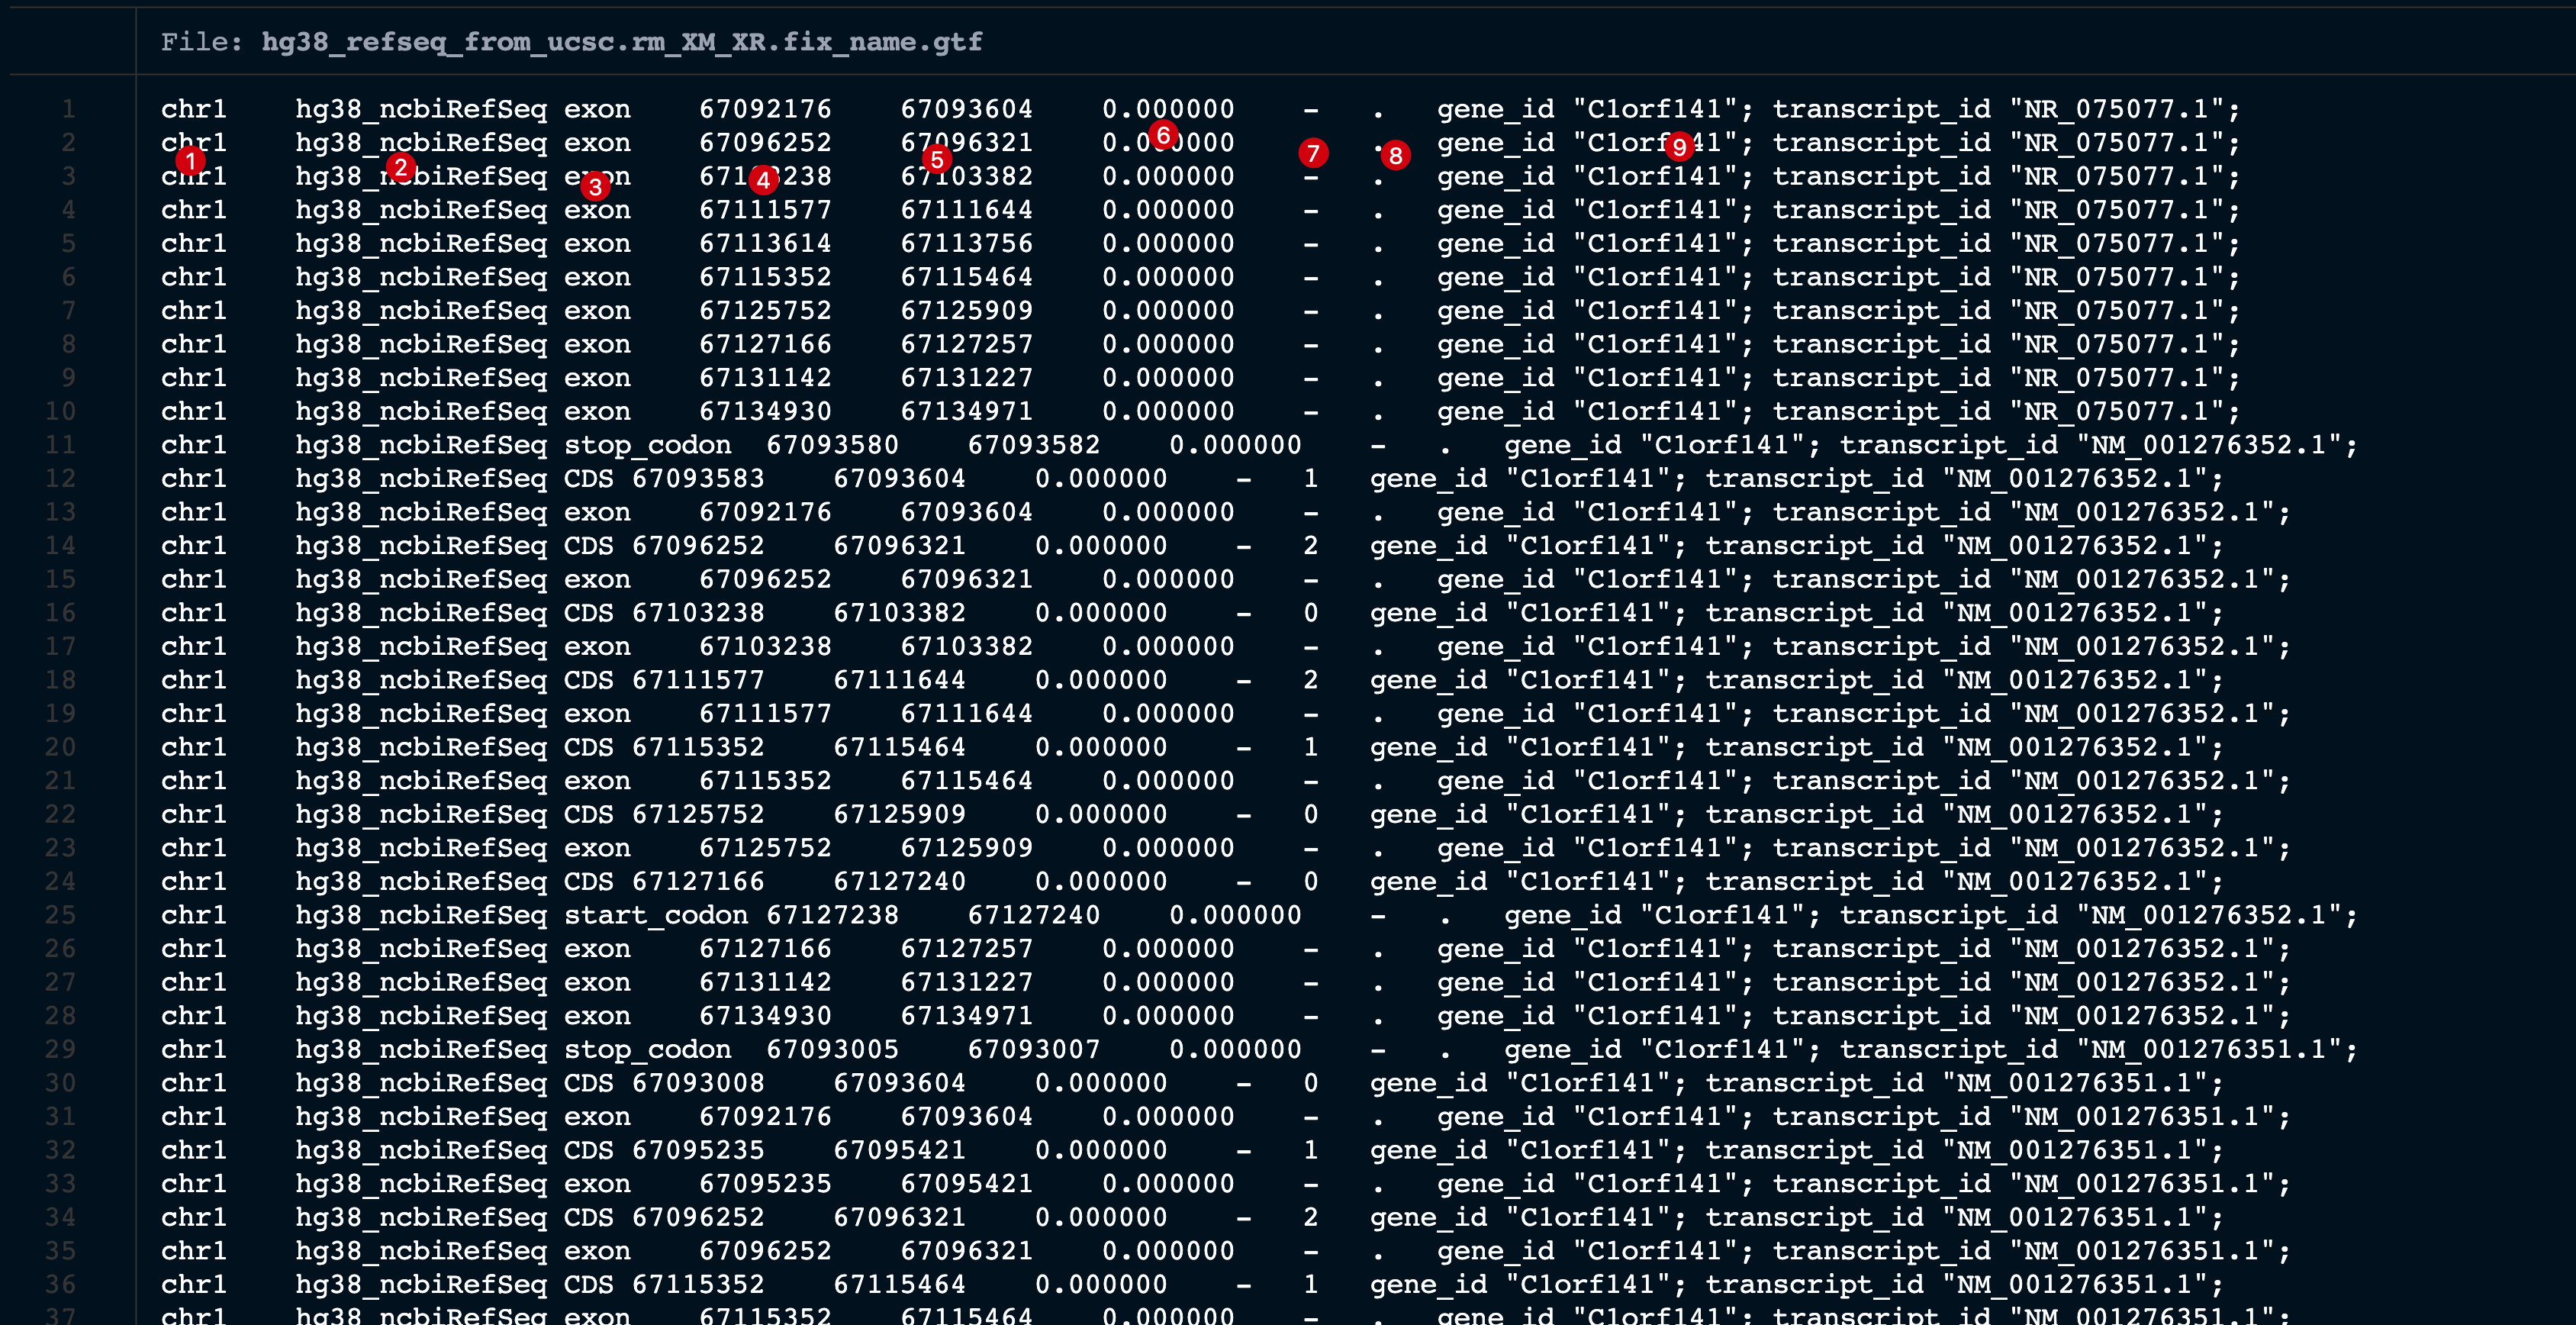
\includegraphics[width=\linewidth]{Images/gtf.png}
    \end{figure}
\end{frame}
\begin{frame}{Demo: another GTF}
    \begin{figure}
        \centering
        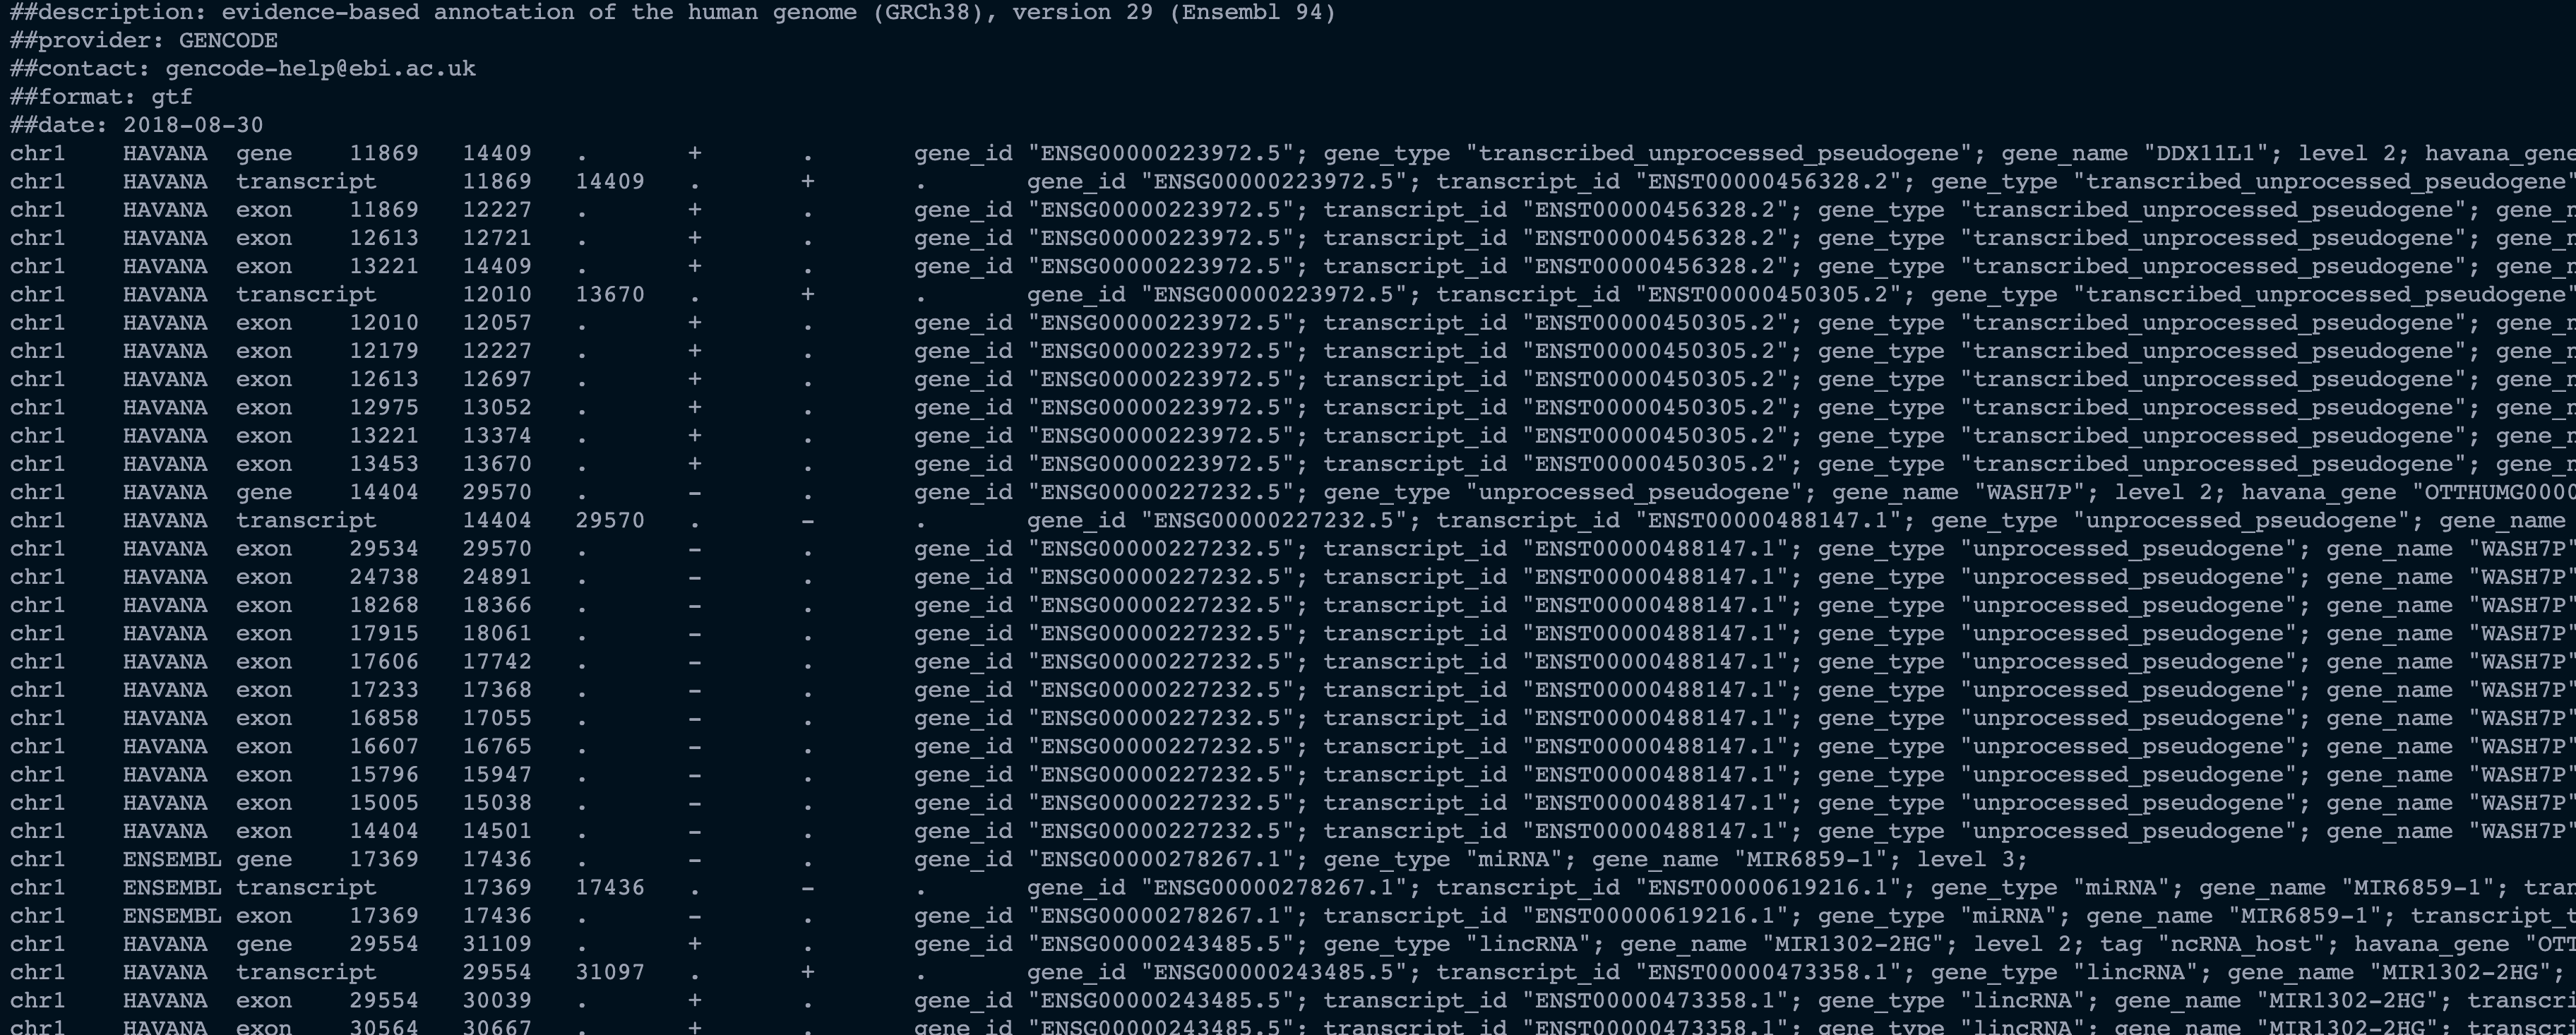
\includegraphics[width=\linewidth]{Images/gtf2.png}
    \end{figure}
\end{frame}

\begin{frame}{Demo: GFF3}
    \begin{figure}
        \centering
        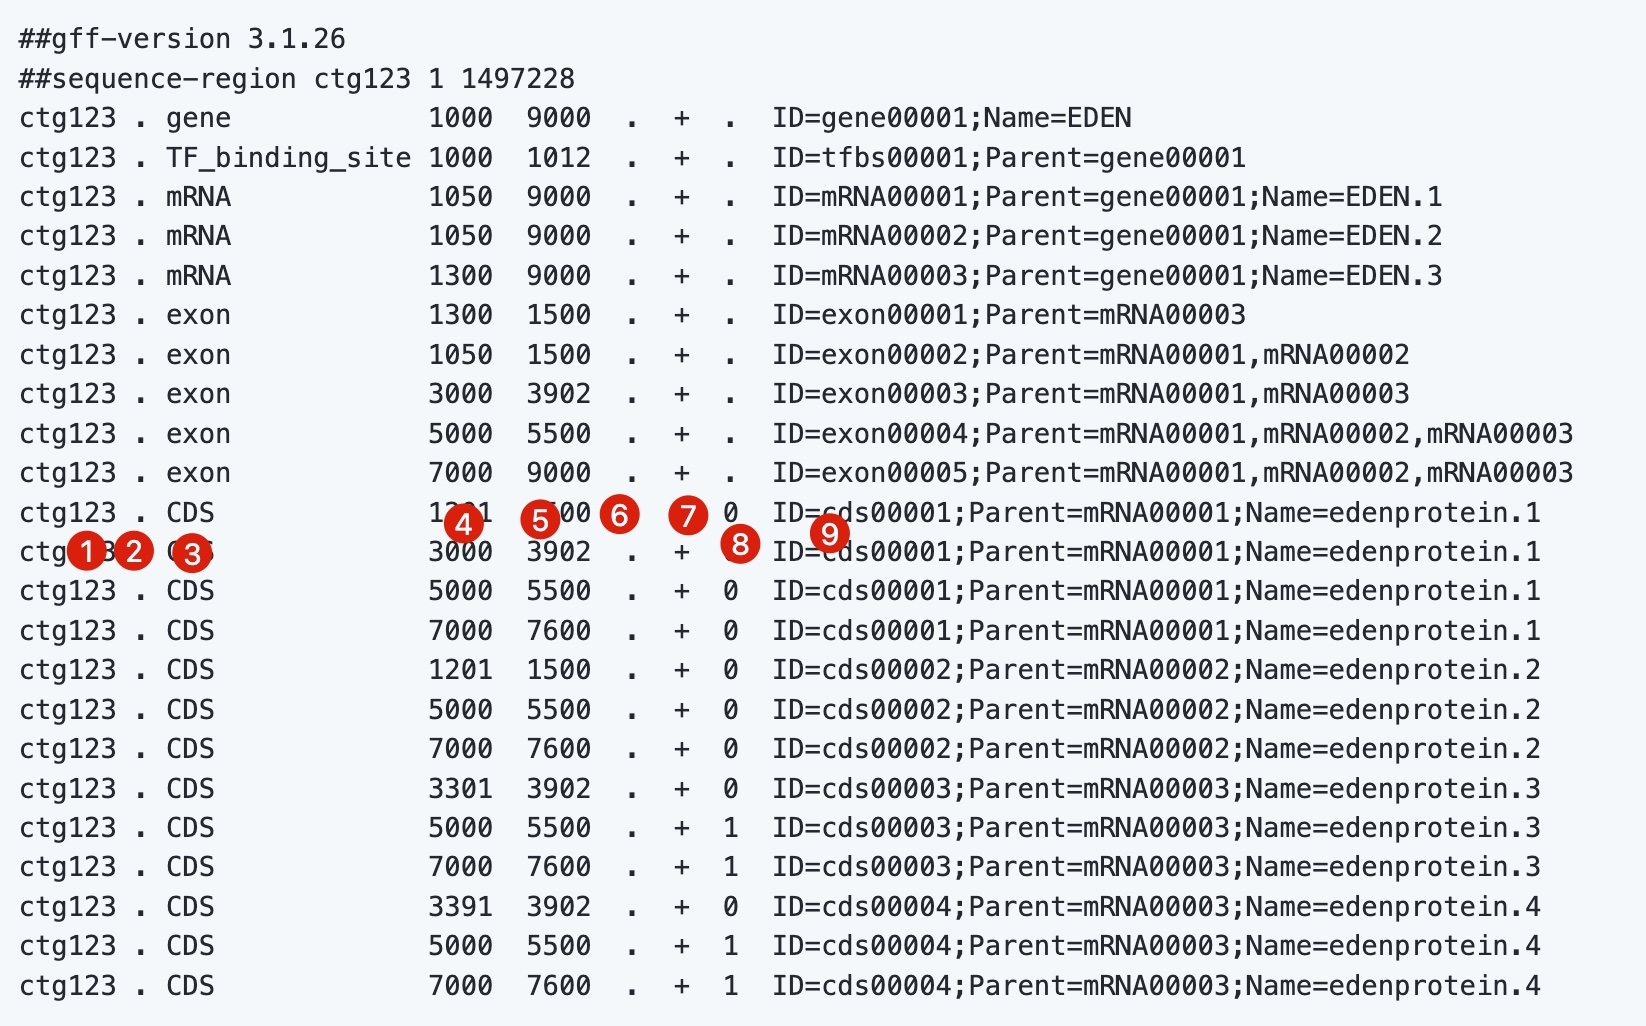
\includegraphics[width=\linewidth]{Images/gff.jpg}
    \end{figure}
\end{frame}


\begin{frame}{Info: 以GTF为例}
    \begin{myoutline}
        \1 1. seq\_id
            \2 序列的编号, 一般为chr或者scanfold编号, 每条染色体拥有一个唯一的ID。
        \1 2. source
            \2 注释的来源, 代表基因结构的来源,可以是数据库的名称,比如来自RefSeq数据库,也可以是软件的名称,比如用GeneScan软件预测得到,当然,也可以为空,用``.''点号填充。
        \1 3. type
            \2 代表区间对应的特征类型, 在GTF中, 常见的类型如下:
                \3 Gene, cDNA, mRNA, 5UTR, 3UTR, exon, CDS, start\_codon, stop\_codon
        \1 4. start
            \2 该基因或转录本在参考序列上的起始位置。
        \1 5. end
            \2 该基因或转录本在参考序列上的终止位置。
        \1 6. score
            \2 得分, 软件提供了统计值, 是注释信息可能性的说明, 可以是序列相似性比对时的E-values值或者基因预测是的P-values值
            \2 ``.''表示为空。
        \1 7. strand
            \2 代表正负链的信息,+表示正链,-表示负链,?表示不清楚正负链的信息
            \2 当正负链信息没有意义时,可以用``.''填充。
    \end{myoutline}
\end{frame}
\begin{frame}{Info: 以GTF为例}
    \begin{myoutline}
        \1 8. phase
            \2 仅对注释类型为``CDS''有效,表示起始编码的位置,有效值为0、1、2
                \3 对于编码蛋白质的CDS来说, 本列指定下一个密码子开始的位置。每3个核苷酸翻译一个氨基酸, 从0开始, CDS的起始位置, 除以3, 余数就是这个值, 表示到达下一个密码子需要跳过的碱基个数。
                \3 0表示该编码框的第一个密码子第一个碱基位于其5'末端
                \3 1表示该编码框的第一个密码子的第一个碱基位于该编码区外
                \3 2表示该编码框的第一个密码子的第一、二个碱基位于该编码区外
            \2 如果\textcolor{red}{Feature为CDS时,必须指明具体值}!
        \1 9. attributes (\textcolor{blue}{更正!})
            \2 一个包含众多属性的列表
                \3 GFF3: 格式为``标签=值'' | ``(tag=value)'', 如果一个序列元件没有Parent属性,说明他的父元件就是scaffold或者chromosome
                \3 GTF: 格式为``标签 值;'' | ``tag value;'',每个特征之后都要有分号(\textcolor{red}{包括最后一个特征})
                \3 GTF: 其内容\textcolor{red}{必须包括gene\_id和transcript\_id}, 其value可以为空``''
    \end{myoutline}
\end{frame}




\begin{frame}[fragile]{GTF和GFF文件操作}
    \begin{columns}
        \column{0.5\textwidth}
        \begin{myoutline}
            \1 ensembl 示例文件下载
                \2 https://www.ensembl.org/
                \2 All genomes (Search 下方)
                \2 选择 Human
                \2 Gene annotation
                \2 Download GTF or GFF3 files for genes, cDNAs, ncRNA, proteins
        \end{myoutline}
        \column{0.5\textwidth}
        \begin{figure}
            \centering
            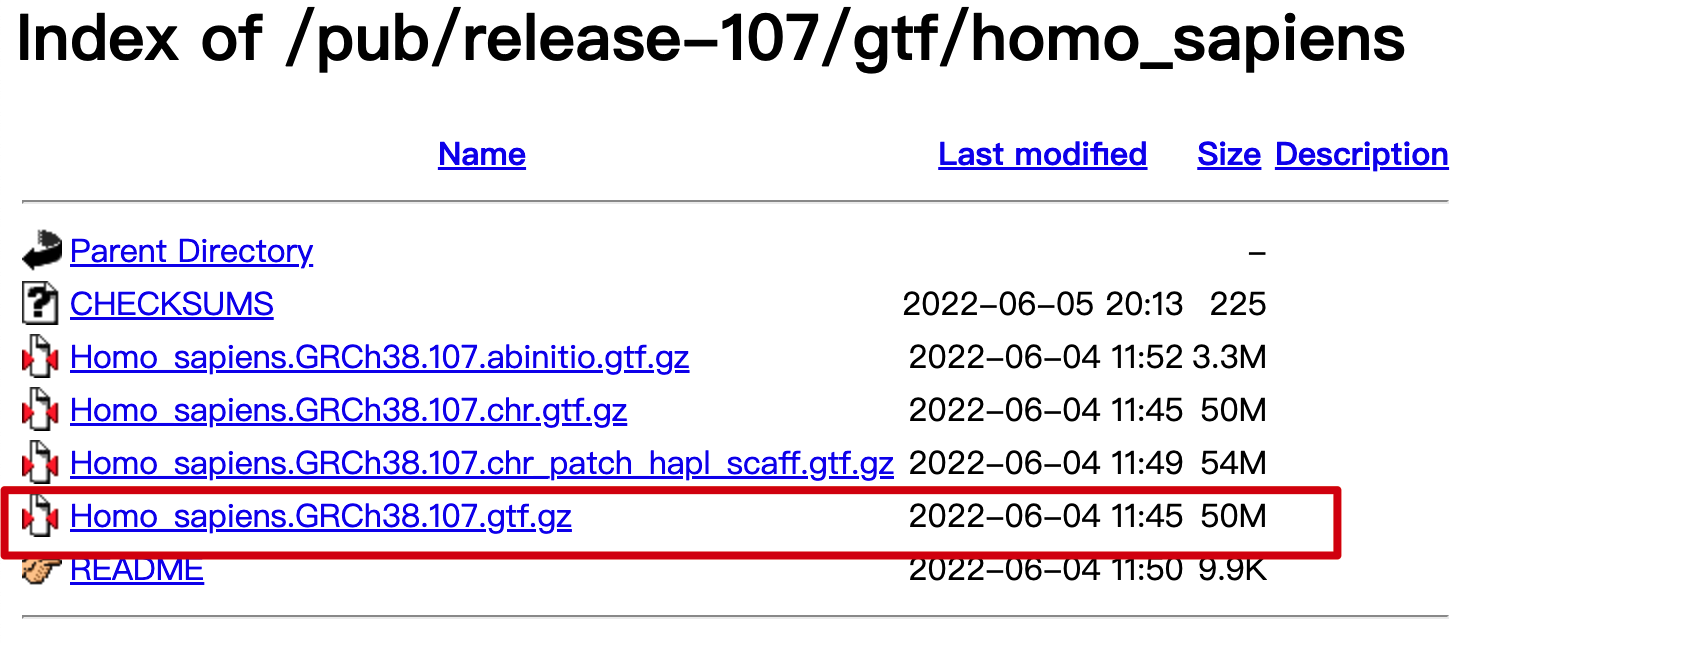
\includegraphics[width=\linewidth]{Images/gtf_download.png}
        \end{figure}
    \end{columns}
    \footnotenoindex{https://www.ensembl.org/}
\end{frame}
\subsection{GTF和GFF文件操作}

\begin{frame}[standout] GTF和GFF文件操作 \end{frame}

\begin{frame}[fragile]{Demo: GFF3 feature}
    % \begin{figure}
    %     \centering
    %     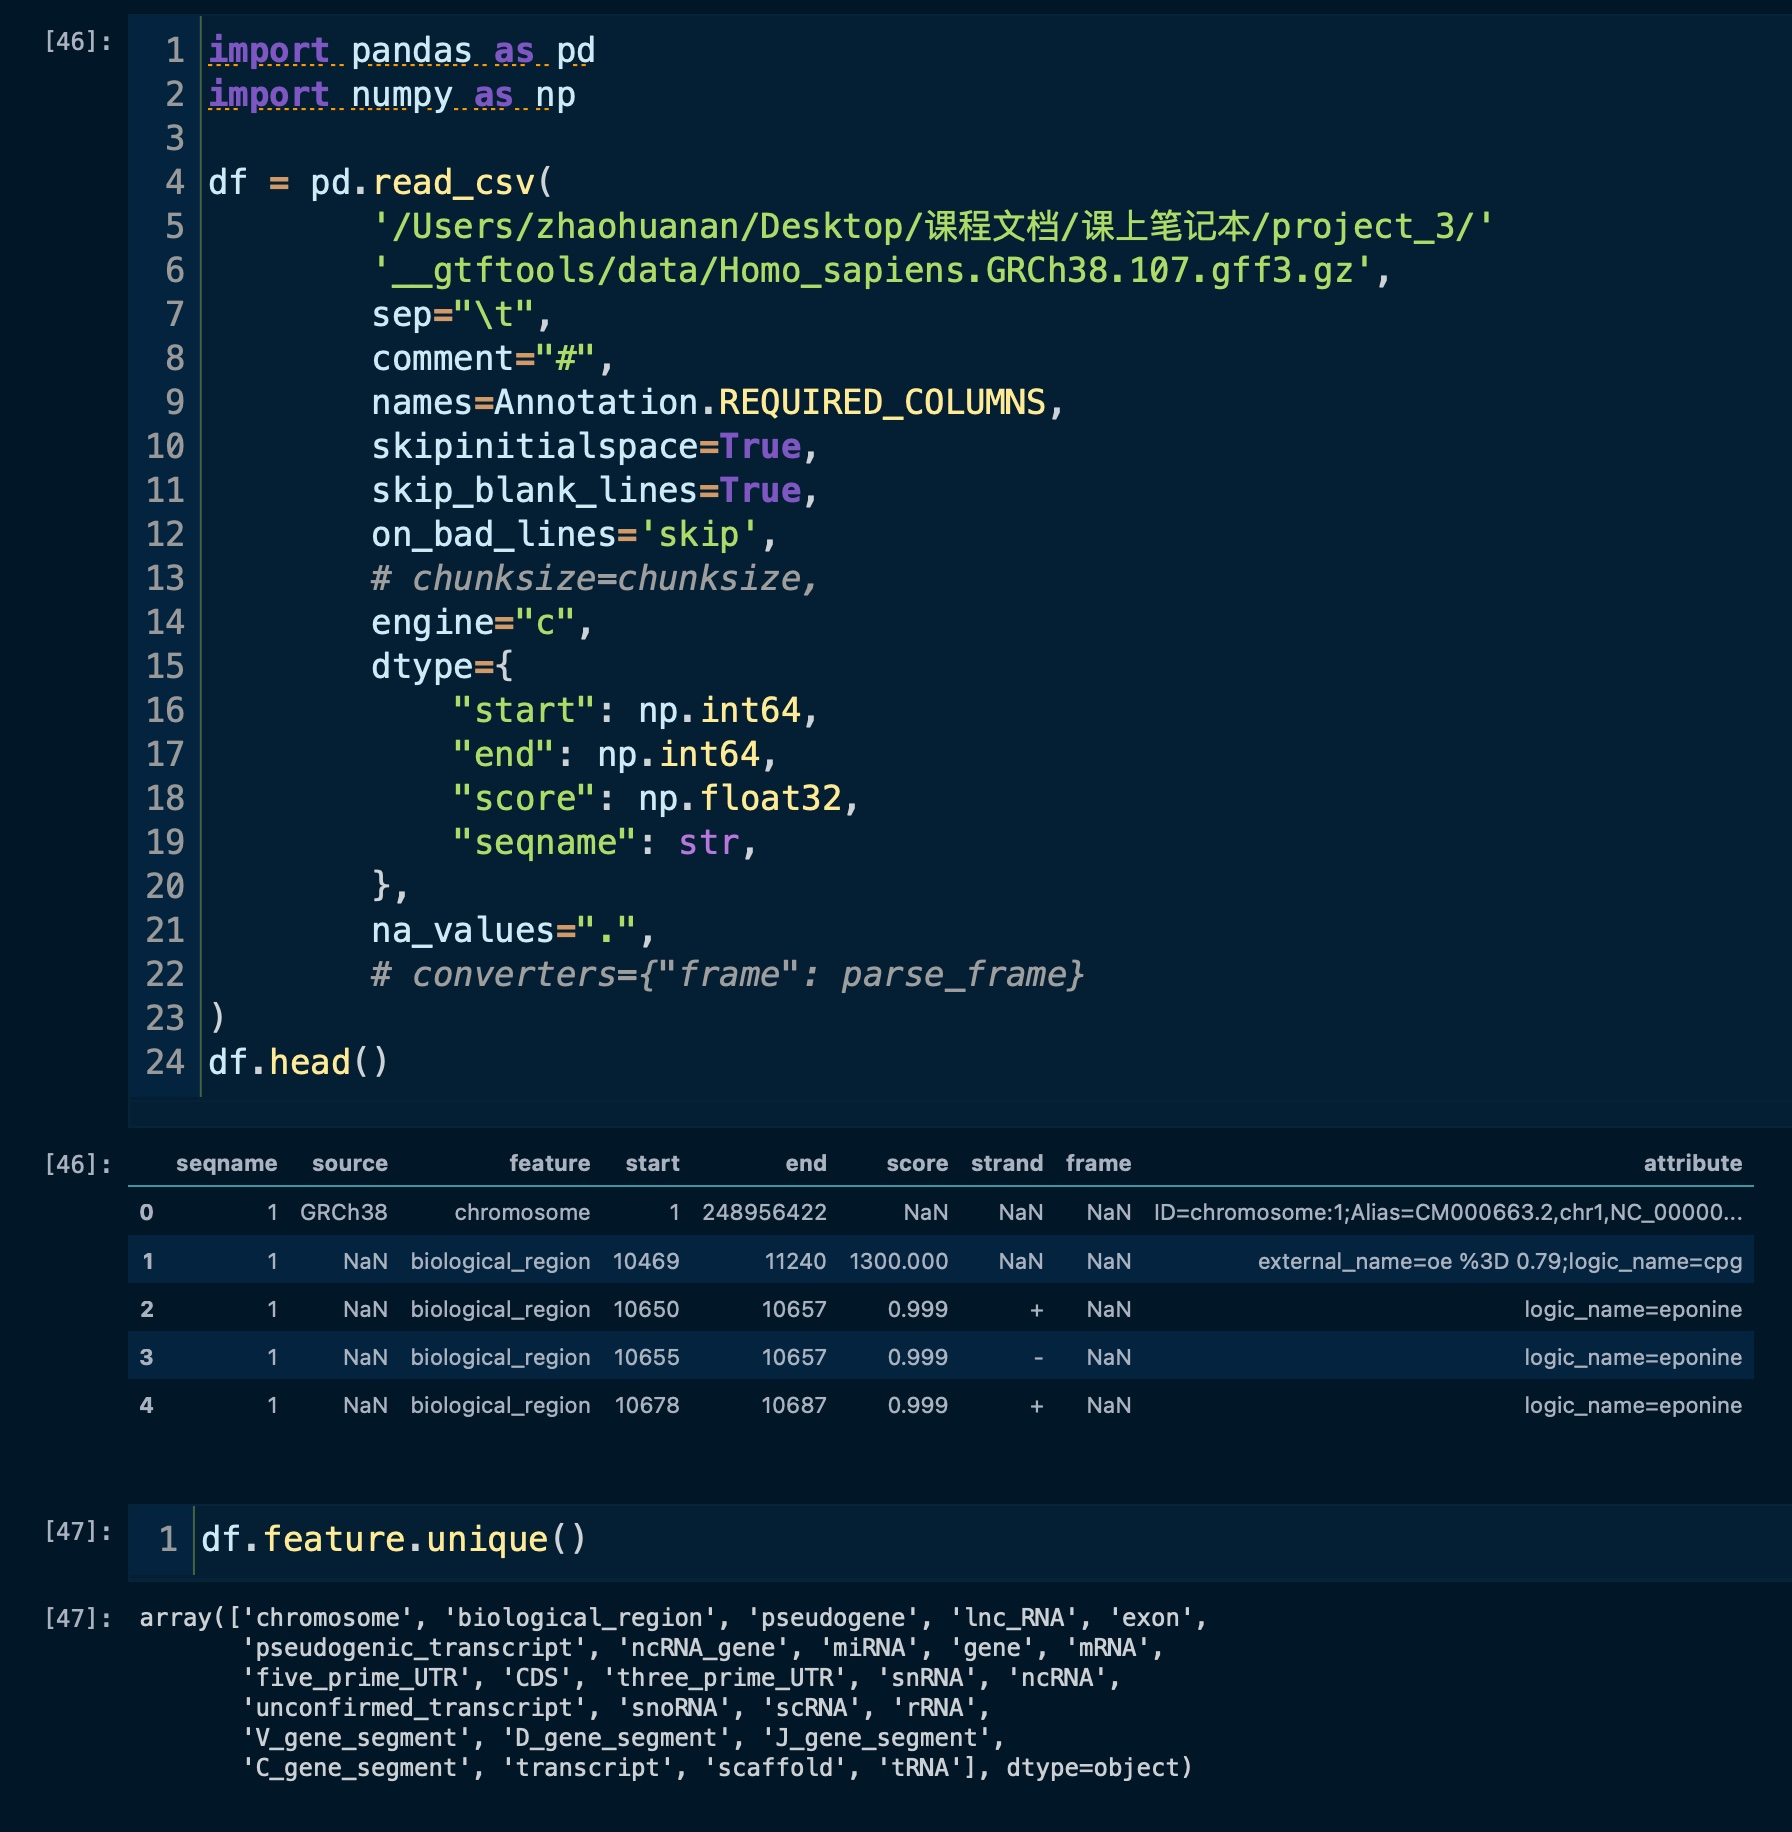
\includegraphics[width=5cm]{Images/gff3_feature.jpg}
    % \end{figure}
    \begin{lstlisting}
import pandas as pd
import numpy as np

df = pd.read_csv(
        'data/Homo_sapiens.GRCh38.107.gff3.gz',
        sep="\t",
        comment="#",
        names=Annotation.REQUIRED_COLUMNS,
        skipinitialspace=True,
        skip_blank_lines=True,
        on_bad_lines='skip',
        # chunksize=chunksize,
        engine="c",
        dtype={
            "start": np.int64,
            "end": np.int64,
            "score": np.float32,
            "seqname": str,
        },
        na_values=".",
)
    \end{lstlisting}
\end{frame}

\begin{frame}[standout] GTF和GFF文件操作 \end{frame}

\begin{frame}[fragile]{Demo: GFF3 feature}
    % \begin{figure}
    %     \centering
    %     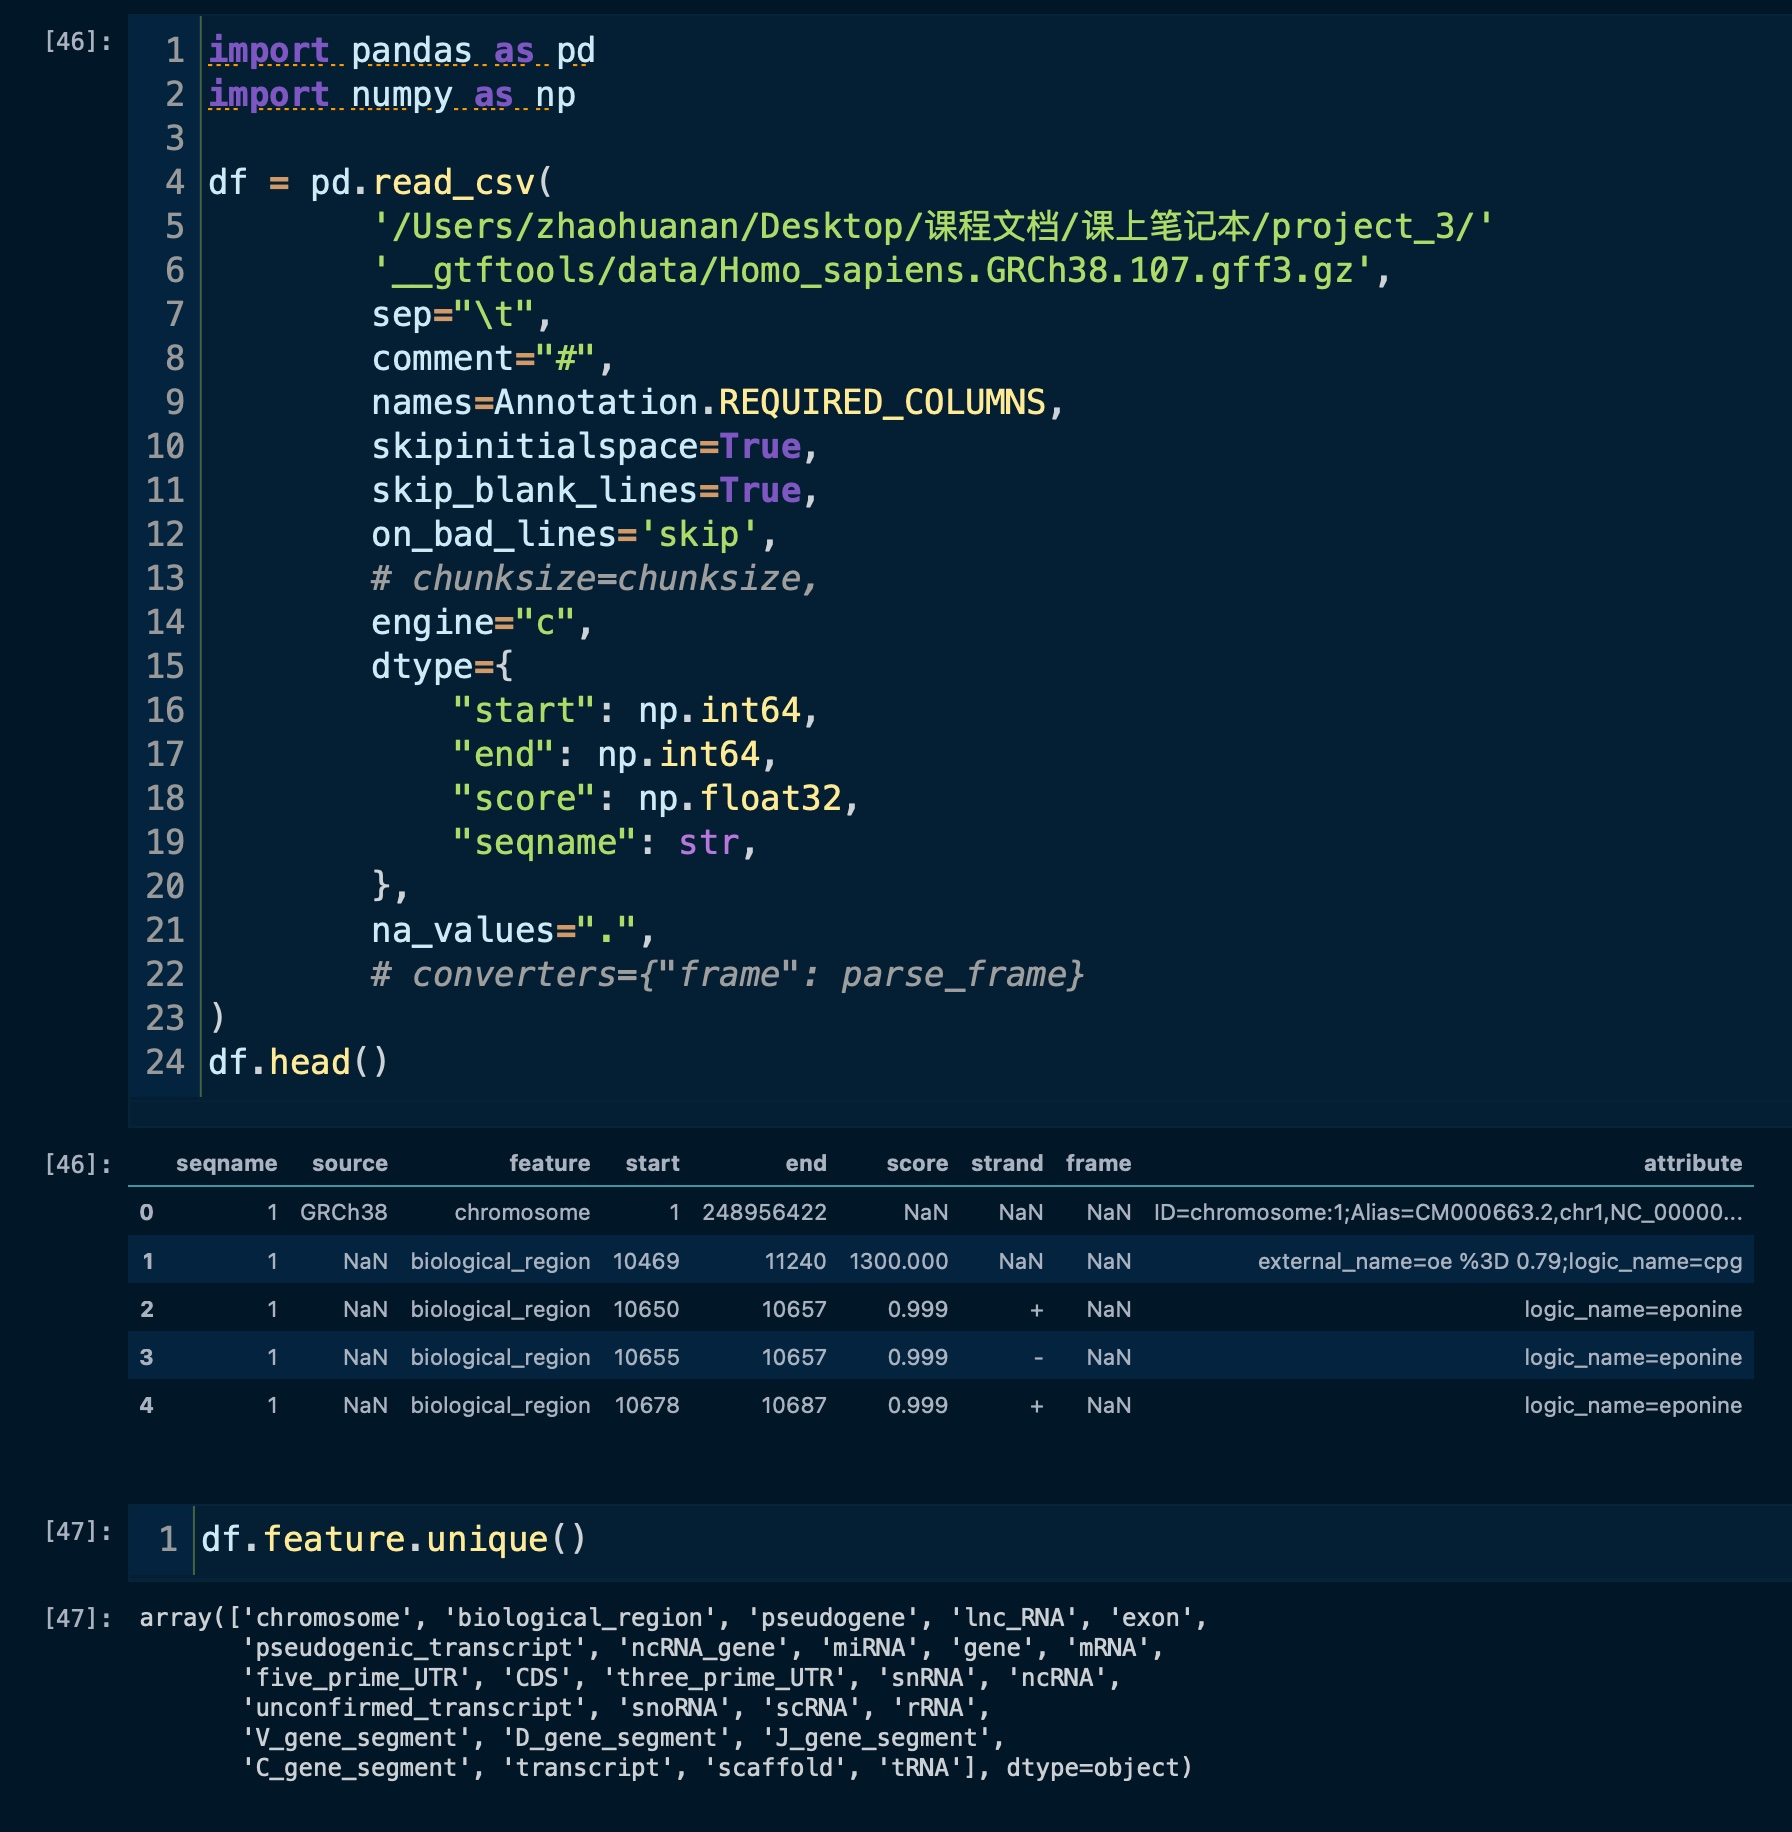
\includegraphics[width=5cm]{Images/gff3_feature.jpg}
    % \end{figure}
    \begin{lstlisting}
df.feature.unique()
array(['chromosome', 'biological_region', 'pseudogene', 'lnc_RNA', 'exon',
       'pseudogenic_transcript', 'ncRNA_gene', 'miRNA', 'gene', 'mRNA',
       'five_prime_UTR', 'CDS', 'three_prime_UTR', 'snRNA', 'ncRNA',
       'unconfirmed_transcript', 'snoRNA', 'scRNA', 'rRNA',
       'V_gene_segment', 'D_gene_segment', 'J_gene_segment',
       'C_gene_segment', 'transcript', 'scaffold', 'tRNA'], dtype=object)

# feature required: 
# - "CDS", 
# - "start_codon"  # 简化,先不考虑,其实是CDS前三个碱基
# - "stop_codon"  # 简化,先不考虑

# optional:
# - "5UTR", 
# - "3UTR",
# - "*RNA"
    \end{lstlisting}
\end{frame}


\begin{frame}[fragile]{练习}
    \begin{lstlisting}
- 仅在必要时才对 self 或 cls 注释(实战课三当中进行讲解)
- cls + @classmethod
- GFF与GTF文件进行转换

- 统计各条染色体的基因密度
- 获得基因的的TSS, TES及启动子坐标 (GFF3)
- 计算全基因组可转录区域长度及所占基因组比例 (GFF3, GTF)
- 计算基因的转录长度、外显子数目及翻译区长度 (GFF3)
    - 计算基因的转录长度
        - 统计平均长度,中位数长度
    - 计算基因的外显子(exon)个数
        - 统计平均个数,中位数个数
        - 统计最多exon的基因, 最少exon的gene
- 程序 CLI 化
    - sys.argv
    - argparse
    \end{lstlisting}
\end{frame}
\subsection{程序CLI化}

\begin{frame}[standout] 程序CLI化 \end{frame}
\begin{frame}[fragile]{程序CLI化}
    % argv
    % argparse
\end{frame}
\begin{frame}[standout] Q \& A! \end{frame}
\begin{frame}[standout] Thank you! \end{frame}

\section{项目实战五 支持多核计算程序的编写}
\subsection{项目实战五 支持多核计算程序的编写}

\begin{frame}[standout] 项目实战五 \quad 支持多核计算程序的编写 \end{frame}

\begin{frame}[standout] 多进程与多线程 \end{frame}

\begin{frame}{多线程与多进程的概念}
    \begin{columns}
        \column{0.5\textwidth}
        \begin{myoutline}
            \1 一个 \textcolor{red}{CPU 核心}
                \2 一条铁轨!
                \2 进行计算的物理硬件
            \1 一个\textcolor{red}{进程(process)} 
                \2一列火车!
                \2 进程是资源分配的最小单位
                \2 不同进程间数据很难共享(一辆火车上的乘客很难换到另外一辆火车,比如站点换乘)
            \1 一个\textcolor{red}{线程(thread)}
                \2 一节车厢!
                \2 线程是CPU调度的最小单位
                \2 单个CPU在任一时刻只能执行单个线程,只有多核CPU还能真正做到多个线程同时运行
                \2 同一进程下不同线程间数据很易共享(A车厢换到B车厢很容易)
        \end{myoutline}
        \column{0.5\textwidth}
        \begin{figure}
            \centering
            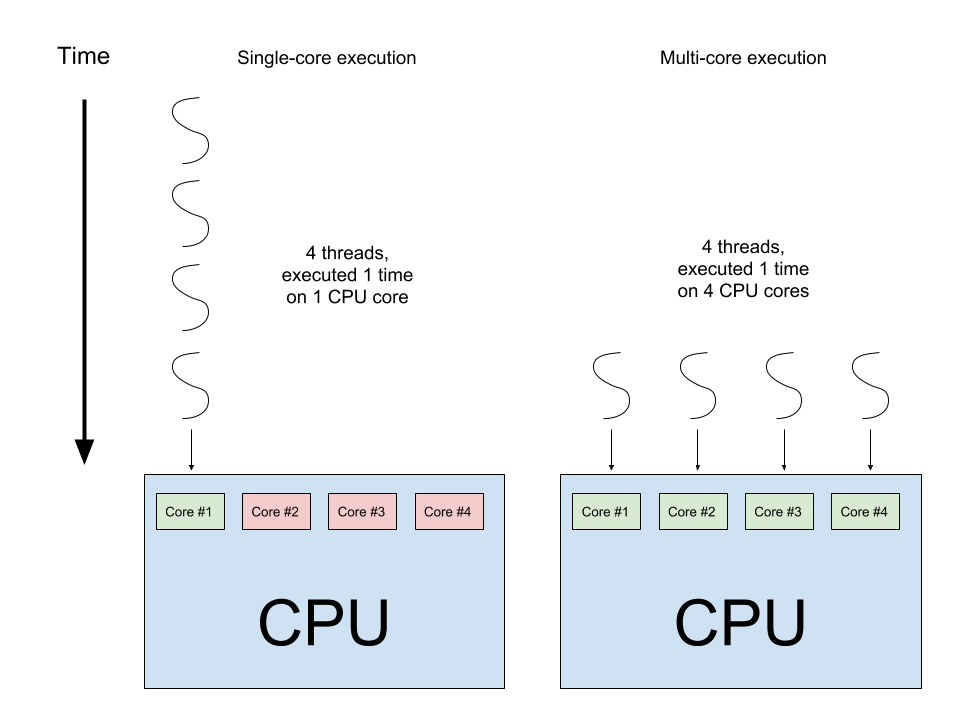
\includegraphics[width=0.9\linewidth]{Images/core_cores.png}
        \end{figure}
    \end{columns}

    \footnotenoindex{https://www.zhihu.com/question/25532384/answer/411179772}
    \footnotenoindex{https://blog.csdn.net/Victor2code/article/details/109005171}
    
\end{frame}

\begin{frame}{多进程与多线程}
    \begin{myoutline}
        \1 进程与线程的关系
            \2 线程在进程的管理下行进
                \3 单纯的车厢无法运行
            \2 一个进程可以包含多个线程
                \3 一辆火车可以有多个车厢
                \3 每个进程在执行过程中拥有独立的内存单元,而一个进程的多个线程在执行过程中共享内存
            \2 \textcolor{red}{进程要比线程消耗更多的计算机资源}
                \3 采用多列火车相比多个车厢更耗资源
            \2 进程间不会相互影响
                \3 一列火车不会影响到另外一列火车
            \2 一个线程挂掉将导致整个进程挂掉
                \3 一列火车上中间的一节车厢着火了,将影响到所有车厢
        \1 多核
            \2 多核CPU同时运行的线程可以属于单个进程或不同进程
            \2 进程使用的内存地址可以上锁
                \3 即一个线程使用某些共享内存时,其他线程必须等它结束,才能使用这一块内存。-"互斥锁"
        \1 \textcolor{red}{在大多数编程语言中},切换线程消耗的资源更少
            \2 而\textcolor{blue}{Python是个特例!}
    \end{myoutline}
\end{frame}


\begin{frame}{GIL锁}
    \begin{columns}
        \column{0.5\textwidth}
        \begin{myoutline}
            \1 GIL锁
                \2 Global Interpreter Lock, 全局解释器锁
                \2 GIL规定, 在一个进程中每次只能有一个线程在运行,也就是一个进程一把 GIL 锁
                    \3 这个GIL锁相当于是线程运行的资格证,某个线程想要运行,首先要获得GIL锁
                    \3 然后遇到IO或者超时的时候释放GIL锁, 给其余的线程去竞争
                    \3 竞争成功的线程获得GIL锁得到下一次运行的机会
            \1 GIL是个历史遗留问题
                \2 GIL的存在, 导致python的多线程其实是假的,所以才有人说python的多线程非常鸡肋
                \2 进程和进程之间会不会受影响?
                    \3 不会
        \end{myoutline}
        \column{0.5\textwidth}
        \begin{figure}
            \centering
            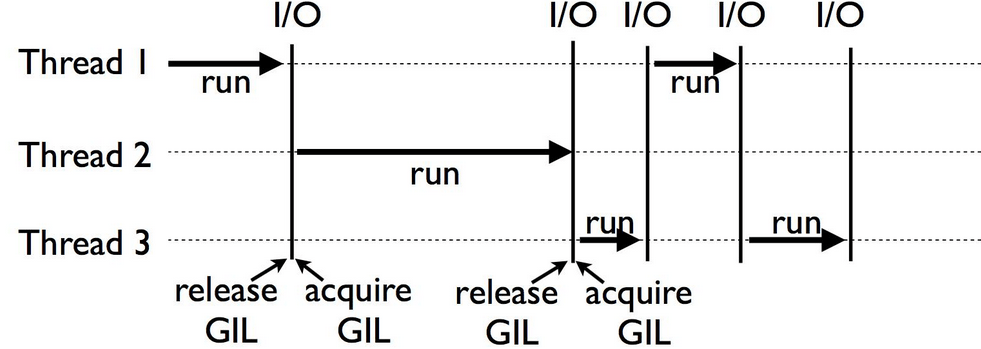
\includegraphics[width=0.9\linewidth]{Images/gil.png}
        \end{figure}
    \end{columns}
\end{frame}

\begin{frame}{由于 GIL 锁的存在}
    \begin{myoutline}
        \1 由于 GIL 锁的存在\dots
        \2 CPU密集型操作使用多进程比较合适, 例如海量运算, 测序 reads 比对到基因组, 计算给定区域的FPKM
        \2 IO密集型操作使用多线程比较合适, 例如爬虫, 超多文件处理
        \2 协程是线程的扩展, 进一步压榨 CPU 的算力(了解,可查阅 asyncio)
    \end{myoutline}
\end{frame}

\begin{frame}[standout]{练习多进程和多线程}
    \begin{myoutline}
        \1 多进程
        \1 多线程
        \1 进程的开销与线程的开销
        \1 进程池 Pool类
            \2 apply \& apply\_async
            \2 map \& map\_async
            \2 close, join, terminate
    \end{myoutline}
\end{frame}



% ————————————————
% 版权声明:本文为CSDN博主「T型人小付」的原创文章,遵循CC 4.0 BY-SA版权协议,转载请附上原文出处链接及本声明。
% 原文链接:https://blog.csdn.net/Victor2code/article/details/109005171
\subsection{计算给定区域的FPKM/RPKM/CPM信号-多核版}

\begin{frame}[standout] 计算给定区域的FPKM/RPKM/CPM信号-多核版 \end{frame}


\subsection{多核程序的性能分析}

\begin{frame}[standout]{多核程序的性能分析}
    使用 1 个核心和多个核心的比较
 \end{frame}


\begin{frame}{一些优质图书}
    \begin{myoutline}
        \1 Python 高性能优化
            \2 流畅的 Python
            \2 Effective Python
        \1 Python 做数据分析
            \2 利用 Python 进行数据分析
            \2 深入浅出 Pandas
    \end{myoutline}
\end{frame}
\begin{frame}[standout] Q \& A! \end{frame}
\begin{frame}[standout] Thank you! \end{frame}
\end{document}

